% !TEX Program = xelatex
\documentclass[master, vlined]{DissertUESTC}



\begin{document}
	
	% 以下两条命令为高亮示例文档中的关键内容而设，正式撰写时切不可使用
	\newcommand{\shad}[1]{\textcolor{DodgerBlue}{\ttfamily #1}}
	\newcommand{\shadcmd}[1]{\shad{$\backslash$#1}}
	
	
	% 下方命令允许跨页排版包含多个行间公式的公式组，可选参数可取值为1,2,3,4，越大表示跨页倾向越高
	% \allowdisplaybreaks[3]
	
	
	% 当论文中某节的内容接近填满页面且其下紧随几项标题时，LaTeX更倾向于在后续的标题前分页，并且纵向拉伸当前页内容的段间距，以实现纵向分散对齐，也就是很多人在问的现象。这并不是模板bug，而是LaTeX特性。
	% 出现这种情况的本质原因是用户的内容，尤其是在页面中有些图、表、标题的时候，它们的高度很可能不是正文行距的整数倍，那必然就会出现这种问题。
	% 如果你觉得Word从上到下直接堆叠内容，然后在页尾留下明显空白的处理方式更合你意，那就使用下方的\raggedbottom命令
	\raggedbottom  % 此命令可让LaTeX像Word那样直接堆叠页面内容，而不再默认拉伸段间距，代价是页尾可能会有明显空白
	
	
	% \setconfidential命令用于设置论文封面中的“密级信息”。慎用！！！学生个人不应随意将论文定性为涉密，需要先经过审批。此命令必须先于\uestccover使用才有效
	% 命令参数：\setconfidential（<信息右上角与纸张左、上边界的距离，以逗号分隔>）[<字体格式>]{<密级>}{<保密期限>}。可选参数默认值：（18cm,2cm）[\zihao{4}\bfseries]
	% \setconfidential{密级}{保密期限}  % 非涉密论文一定要注释掉该命令
	
	% 封面示例————“双学位学士”以外的学位论文
	%	\uestccover[<学院名称排版风格>]{<论文题目>}{<学科专业>}{<学号>}{<作者姓名>}{<指导教师>}{<教师职称>}{<学院>} % 单学位学士、研究生通用
	\uestccover{}{}{}{}{}{}{}  % 空封面
	
	% \uestccover{基于RISC-V的微内核虚拟化方案研究}
	% {计算机科学与技术}
	% {202321081001}
	% {李金哲}
	% {罗蕾}
	% {教\hspace{1em}授}%{终南山古墓派}
	% { 	信息与软件工程学院（示范性软件学院）}  % 默认将过长的学院名称压缩至下划线宽度
	
	% \uestccover[par]{关于我的杀父仇人疑似是名震天下的大侠时该如何报仇}
	% 			{玉女素心剑法}
	% 			{1182000}
	% 			{杨\hspace{1em}过}
	% 			{小龙女}
	% 			{掌\hspace{1em}门}%{终南山古墓派}
	% 			{终南山古墓派终南山古墓派终南山古墓派}  % par参数将过长学院名称换行排版，此参数必影响封面布局，无可避免
	
	% 封面示例————“双学位学士”论文，需要doublebachelor选项
	% \uestccover{<论文题目>}{<学院>}{<第一专业>}{<第二专业>}{<学号>}{<作者姓名>}{<第一导师及职称>}{<第二导师及职称>} % 仅双学位学士论文，需要doublebachelor选项
	% \uestccover{}{}{}{}{}{}{}{}  % 空封面
	% \uestccover{关于我的杀父仇人疑似是名震天下的大侠时该如何报仇}
	% 			{终南山古墓派终南山古墓派终南山古墓派}  % 空间有限，过长的学院名称必须压缩至下划线宽度
	% 			{玉女素心剑法}
	% 			{打狗棒法}
	% 			{1182000}
	% 			{杨\hspace{1em}过}
	% 			{小龙女\hspace*{4em}掌\hspace{1em}门}
	% 			{洪七公\hspace*{4em}帮\hspace{1em}主}
	
	
	
	% 中文扉页，仅研究生用
	% \DegLv{}  % 清空文档类选项设置的<申请学位级别>
	% \Author{李金哲}
	% \DissertationTitle{基于RISC-V的微内核虚拟化方案研究}
	% \Supervisor{罗蕾}{教\hspace{1em}授}{电子科技大学}{成都}
	% \Major{计算机科学与技术}
	\uestczhtitlepage  % 空白中文扉页

	% \ClsNum{TN828.6}  % \ClsNum{<分类号>}
	% \ClsLv{公开}  % \ClsLv{<密级>}
	% \UDC{621.39}  % \UDC{<UDC号>}
	% \DissertationTitle{关于我的杀父仇人疑似是名震天下的大侠时\\该如何报仇}  % \DissertationTitle{<题名>}
	% \Author{杨过}  % \Author{<作者姓名>}
	% \Supervisor{小龙女}{掌门}{古墓派}{活死人墓}  % \Supervisor{<指导教师$ $>}{<职称>}{<单位名称>}{<单位地址>}
	% % 副导师信息，无则注释
	% \AssociateSupervisor{洪七公}{前帮主}{丐帮}{襄阳}  % \AssociateSupervisor{<副导师名称>}{<职称}>{<单位名称>}{<单位地址>}
	% \DegLv{西狂}  % \DegLv{<申请学位级别>}，该信息由文档类选项自动确定，需修改默认内容时使用，否则注释即可
	% \Major{玉女素心剑法}  % \Major{<学科专业>}
	% \Profield{剑道}  % \Profield{专业学位领域代码}，此为专业学位独有，学术学位用户注释即可
	% \Date{1959年1月1日}{1961年1月1日}  % \Date{<论文提交日期>}{<论文答辩日期>}
	% \Grant{中华武林}{1961年2月2日}  % \Grant{<学位授予单位>}{<学位授予日期>}
	% \Reviewer{黄蓉}{一灯大师、老顽童、黄老邪、郭靖、小龙女}  % \Reviewer{<答辩委员为主席>}{<评阅人>}
	% \uestczhtitlepage
	
	
	% \Supervisor{小龙女}{古墓派末代掌门}{古墓派}{活死人墓}  % \Supervisor{<指导教师>}{<职称>}{<单位名称>}{<单位地址>}
	% % 副导师信息，无则注释
	% \AssociateSupervisor{洪七公}{天下第一帮前帮主}{丐帮}{襄阳}  % \AssociateSupervisor{<副导师名称>}{<职称}>{<单位名称>}{<单位地址>}
	% \Reviewer{黄蓉}{一灯大师、老顽童、黄老邪、郭靖、小龙女、金轮法王、洪七公、欧阳锋}  % \Reviewer{<答辩委员为主席>}{<评阅人>}
	% \uestczhtitlepage  % 过长评阅人文本将被自动压缩至下划线宽度，不会超出页面边界
	
	% \uestczhtitlepage[compress]  % 在compress选项下，“中文扉页”将自动压缩过长职称的字宽，使之不超出官方模板为该内容设定的长度
	
	
	% 英文扉页，仅研究生用
	\uestcentitlepage{}{}{}{}{}{}{}
	
	% \uestcentitlepage{Research on RISC-V-Based Microkernel Virtualization Architecture}{Computer Science and Technology}{202321081001}{Li Jinzhe}{Prof.Luo Lei}{}{School of Information and Software Engineering}  % 空白英文扉页
	
	% \uestcentitlepage{How to Take Revenge When My Father's Murderer is Suspected to Be a Famous Hero}
	% 				{Jade Lady Soul Sword Technique Jade Lady Soul Sword Technique}
	% 				{1182000}
	% 				{Yang Guo}
	% 				{Grandmaster Dragondaughter Little}{Grandmaster Northern Beggar}
	% 				{Ancient Tomb Sect Ancient Tomb Sect Ancient Tomb Sect Ancient Tomb Sect}
	
	% 独创性声明：[<签名宽度>]{<日期>}{<作者签名图片1>}[<作者签名图片2 默认值为作者签名图片1>]{<导师签名图片>}，仅研究生用
	
	\declaration[3cm]{}{}{}
	
	
	% 开启中文摘要
	\zhabstract
	随着边缘异构计算的发展，嵌入式系统面临数据安全与隐私泄露挑战。机密虚拟机（CVM）作为保障敏感数据与模型资产的核心技术，已成为机密计算领域的研究热点。然而，现有商用CVM架构多受限于闭源体系，且传统基于C/C++构建的底层安全固件易受内存破坏漏洞的威胁。此外，在资源受限的端侧环境中，兼顾隔离安全性与异构设备的复用效率仍是当前面临的技术挑战。针对上述问题，本文基于开源RISC-V 指令集架构，设计并实现了一套微内核机密虚拟化系统EasyAda-trust。本文的主要研究工作如下：
	
	1.提出了一种基于Rust内存安全特性的底层可信固件架构。 结合Rust所有权机制重构页分配器，通过编译期静态检查消除二次释放等内存隐患；同时，将RISC-V物理内存保护（PMP）机制抽象为统一的内存保护原语，实现CVM与不可信组件间的硬件级隔离，构建系统底层信任根。
	
	2.构建了支持CVM全生命周期的软硬协同虚拟化机制。实现了物理资源调度与安全鉴权的解耦。不可信Hypervisor负责宏观资源分配，而安全区域构建、二阶段页表映射及机密执行流的上下文切换等敏感操作，均由TEE安全管理器（TSM）代理执行。此外，结合本地证明机制实现了CVM与硬件环境的双向信任度量。
	
	3. 设计了防范DMA攻击的端侧机密异构计算环境。 在EasyAda-trust中引入RISC-V IOPMP硬件扩展支持，在总线级实施外设动态鉴权与细粒度访问控制。在此基础上，构建加速器管理CVM，利用I/O半虚拟化与安全共享内存映射技术建立跨域信道，使机密应用能够旁路不可信软件栈，实现底层硬件加速器在机密环境内的零拷贝明文复用。
	
	最后，在QEMU仿真环境下对系统开展了多维度量化评估。实验结果表明，EasyAda-SM能够以较小的代价兼容现有RISC-V TEE方案，其核心计算（CoreMark与 RV8）性能损耗低于2\%，验证EasyAda-SM的可拓展性；得益于静态内存预分配机制，EasyAda-trust中CVM在系统时钟与访存等核心原语上的执行开销与原生系统相近；同时，安全直通架构有效保障了异构I/O的吞吐效率。评估结果表明，本文方案在内存安全性、异构设备复用率与总体计算效能之间实现了合理的架构折中，为端侧机密计算的部署提供了系统级解决方案。
	\zhkeywords{Rust，RISC-V，微内核虚拟化，机密计算，可信异构计算}
	
	
	% 开启英文摘要
	\enabstract
	With the rapid development of edge heterogeneous computing, embedded systems face severe challenges regarding data security and privacy leakage. As a core technology to safeguard sensitive data and high-value model assets, the Confidential Virtual Machine (CVM) has become a research hotspot in the field of confidential computing. However, existing commercial CVM architectures are mostly constrained by closed-source ecological barriers, and traditional underlying security firmware built with C/C++ suffers from critical memory safety vulnerabilities. Furthermore, achieving a balance between high-security isolation and the efficient reuse of heterogeneous devices in resource-constrained edge environments remains an urgent technical challenge. To address these pain points, this thesis designs and implements EasyAda-trust, a microkernel-based confidential virtualization system based on the open-source RISC-V instruction set architecture. The main research work and innovations of this thesis are as follows:
	
	1. Proposed an underlying trusted firmware architecture based on the memory safety features of Rust. By deeply integrating Rust's ownership mechanism to reconstruct the page allocator, memory vulnerabilities such as Double-Free are statically eliminated at compile time. Meanwhile, the RISC-V Physical Memory Protection (PMP) mechanism is abstracted into a unified security primitive, constructing a hardware-level strong isolation boundary between the CVM and untrusted components, thereby establishing the underlying root of trust of the system.
	
	2. Constructed a hardware-software co-designed virtualization management mechanism supporting the full lifecycle of CVMs. The responsibility decoupling of physical resource scheduling and security authentication is innovatively implemented. The untrusted Hypervisor is solely responsible for macroscopic resource allocation, while core sensitive operations such as secure region construction, two-stage page table mapping, and context switching of confidential execution flows are mediated by the Trusted Security Manager (TSM). In addition, a local attestation mechanism is introduced to realize bidirectional trusted measurement between the CVM and the underlying hardware.
	
	3. Designed an edge confidential heterogeneous computing environment to prevent DMA attacks. By introducing the RISC-V IOPMP hardware extension, peripheral dynamic authentication and fine-grained access control are enforced at the bus level. On this basis, a dedicated "Accelerator Management CVM" is designed. Relying on I/O para-virtualization and secure shared memory mapping technologies to bridge cross-domain channels, confidential applications can bypass the untrusted software stack, successfully achieving the zero-copy plaintext utilization of underlying hardware accelerators within the confidential environment.
	
	Finally, multi-dimensional quantitative evaluations of the system were conducted in the QEMU simulation environment. The experimental results show that EasyAda-SM can be compatible with the existing RISC-V TEE ecosystem with extremely low overhead, and the performance degradation of core computing (CoreMark and RV8) is strictly controlled within 2\%, verifying its excellent scalability. Thanks to the static memory pre-allocation mechanism, the execution overhead of the CVM on core primitives such as system clock and memory access approaches that of the native system. Meanwhile, the secure pass-through architecture effectively guarantees the throughput efficiency of heterogeneous I/O. In summary, the proposed scheme achieves a reasonable architectural trade-off among memory safety, heterogeneous device reuse rate, and overall computing efficiency, providing an effective system-level solution for the generalized deployment of edge confidential computing.
	
	% 英文关键词
	\enkeywords{Rust Language; RISC-V; Microkernel Virtualization; Confidential Computing; Trust Heterogeneous Computing}
	
	
	\tableofcontents  % 主目录，必要
	
	\listoffigures  % 图多则放，反之不放
	
	%\listoftables  % 表多则放，反之不放
	
	% \listofsymbs  % 生成主要符号表标题，需要额外维护符号表内容
	
	% 生成主要符号表的章标题需使用本模板提供的\shadcmd{listofsymbs}命令。排版主要符号表的内容则需要使用本模板提供的\shad{symbtable}环境。该环境基于\shad{longtable}环境进行封装，依次接受两个可选参数：
	
	% \shadcmd{begin\{symbtable\}[<表格整体位置>]（<主要符号表的列控制参数>）}
	
	% \noindent 其中，第一项可选参数用于设置\shad{longtable}环境的可选参数，且默认值与\shad{longtable}环境保持一致；第二项可选参数用于设置\shad{longtable}环境的必选参数，其默认值设置为\shad{p\{3.5em\} p\{$\backslash$linewidth-9em\} p\{3em\}<\{$\backslash$centering\}}。
	
	% 若非必要，用户不应指定\shad{symbtable}环境的可选参数。但若出于对排版美观性的考虑，可适当调整主要符号表各列的宽度。注意，按照学位论文撰写规范中的示例，$1。因此，切勿对第二项可选参数设置其他列数。
	
	% $1：\shadcmd{listofsymbs}命令和\shad{symbtable}环境必须同时出现或消失。不需要主要符号表时，通通注释掉即可；需要时，必须使用\shad{symbtable}环境生成表格内容。
	
	% \begin{symbtable}
		% 	a & 加速度（acceleration） & 1 \\
		% 	A & 振幅（amplitude）、面积（Area）、磁场矢量势（magnetic vector potential） & 2 \\
		% 	B & 磁场、磁感应强度、核结合能 & 3 \\
		% 	c & 真空中光速 & 4 \\
		% 	C & 比热容（heat capacity）、电容 & 5 \\
		% 	d & 长度（distance）、直径（diameter）、微分（differential，如dx）& 6 \\
		% 	D & 电位移矢量（electric displacement） & 7 \\
		% 	e & 元电荷、自然底数（欧拉常数）& 8 \\
		% 	E & 能量、电场场强，电动势 & 9 \\
		% 	f & 频率、焦距（光学） & 10 \\
		% 	F & 力、通量（Flux） & 11 \\
		% 	g &（地表）重力加速度 & 12 \\
		% 	G & 万有引力常数 & 13 \\
		% 	h & 普朗克常数、高度 & 14 \\
		% 	H & 哈勃常数、焓、磁化强度矢量、哈密顿算符（Hamiltonian） & 15 \\
		% 	i & 虚数单位 & 16 \\
		% 	I & 电流、惯量（inertia）、冲量（impulse） & 17 \\
		% 	j & 辐射强度、加加速度（jerk） & 18 \\
		% 	J & 角动量、概率流（量子力学）、电流密度、巨配分函数里的巨势 Z（J） & 19 \\
		% 	k & 玻尔兹曼（Boltzmann）常数、库伦常数、用来指代某常量或固定比值 & 20 \\
		% 	K & 四维波矢量（相对论）、动能 & 21 \\
		% 	l & 长度（length） & 22 \\
		% 	L & 角动量、电感系数 & 23 \\
		% 	m & 质量 & 24 \\
		% 	M & 磁化率 & 25 \\
		% 	n & 序数、主量子数、摩尔数（化学）、折射率（光学） & 26 \\
		% 	N & 序数、中子数、放大倍率（光学）& 27 \\
		% 	o & 小o符号 & 28 \\
		% 	O & 大O符号 & 29 \\
		% 	p & 动量、压强（pressure）、电偶极矩（electric dipole moment） & 30 \\
		% 	P & 概率（量子力学，统计学）、功率（power）、极化度 & 31 \\
		% 	q & 电荷 & 32 \\
		% 	Q & 电荷热量、流量 & 33 \\
		% 	r & 半径、位置向量、球坐标系半径轴 & 34 \\
		% 	R & 电阻、普适气体常数（热力学）、里德伯（Rydberg）常数（光谱学）、反射率（Reflectivity，光学） & 35 \\
		% 	s & 自旋 & 36 \\
		% 	S & 熵、面积 & 37 \\
		% 	t & 时间 & 38 \\
		% 	T & 温度、周期、透射率（Transmittance，光学） & 39 \\
		% 	u & 原子质量单位、物距（光学） & 40 \\
		% 	U & 电压、电势 & 50 \\
		% 	v & 速度、像距（光学） & 51 \\
		% 	V & 体积、势能 & 52 \\
		% 	w & 速度 & 53 \\
		% 	W & 功 & 54 \\
		% 	x & 直角坐标系横轴 & 55 \\
		% 	X & 磁化率、电抗 & 56 \\
		% 	y & 直角坐标系纵轴 & 57 \\
		% 	Y & 光亮度、球谐函数 & 58 \\
		% 	z & 直角/圆柱坐标系竖轴、复数变量 & 59 \\
		% 	Z & 阻抗、原子序数（质子数）、配分函数（partition function） & 60 \\
		% 	$\alpha$ & 角度、精细结构常数、角加速度、四维加速度（相对论）、攻角 & 61 \\
		% 	Α & Alpha （与英文拼写难区分的希腊字母一般不使用） & 62 \\
		% 	$\beta$ & 角度；磁通系数；速度与光速的比值 & 63 \\
		% 	Β & Beta Β函数 & 64 \\
		% 	γ & 电导系数、洛伦兹因子、热容比 & 65 \\
		% 	Γ & Gamma Γ函数、克里斯托弗尔符号 & 66 \\
		% 	δ & 狄拉克δ函数、克罗内克函数（Kronecker delta）、屈光度、微分 & 67 \\
		% 	Δ & Delta 拉普拉斯算子、有限差 & 68 \\
		% 	ε & 电容率（permittivity）、介电常数、列维-奇维塔符号（Levi-Civita symbol）、发射率 & 69 \\
		% 	Ε & Epsilon & 70 \\
		% 	Ϝ & digamma & 71 \\
		% 	ζ & 阻尼比、黎曼ζ函数 & 72 \\
		% 	Ζ & Zeta & 73 \\
		% 	η & 黏度（viscosity）、磁滞系数、效率 & 74 \\
		% 	Η & Eta & 75 \\
		% 	θ & 角变量、温度、球坐标/圆柱坐标横角 & 76 \\
		% 	Θ & Theta 单位阶跃函数（Heaviside step function） & 77 \\
		% 	Ι & Iota & 78 \\
		% 	$\kappa$ & 介质常数比ε/ε0、导热率、热扩散率 & 79 \\
		% 	$\kappa$ & Kappa & 80 \\
		% 	λ & 波长、mean free path、半衰期 & 81 \\
		% 	$\Lambda$ & Lambda 洛伦兹变换、冯·卡门常数 & 82 \\
		% 	μ & 磁导率、质子质量单位、摩擦系数、离子迁移率 & 83 \\
		% 	Μ & Mu & 84 \\
		% 	ν & 频率、运动粘度、自由度 & 85 \\
		% 	Ν & Nu & 86 \\
		% 	ξ & 黎曼ξ函数、随机变量 & 87 \\
		% 	Ξ & Xi & 88 \\
		% 	Ο & Omicron & 89 \\
		% 	π & 圆周率、共轭动量 & 90 \\
		% 	∏ & Pi 乘积 & 91 \\
		% 	ρ & 密度、电阻率 & 92 \\
		% 	Ρ & Rho & 93 \\
		% 	σ & 导电率、斯提芬-波尔兹曼常数（Stefan–Boltzmann constant）、核反应截面、表面密度、标准差 & 94 \\
		% 	∑ & Sigma 总和 & 95 \\
		% 	τ & 扭矩（Torque）、剪应力（Shear stress）、时间常数、2π & 96 \\
		% 	Τ & Tau & 97 \\
		% 	Υ & Upsilon & 98 \\
		% 	φ & 球坐标纵角、波相位（wave phase）、直径 & 99 \\
		% 	Φ & Phi 磁通量、辐射通量、逸出功 & 100 \\
		% 	χ & 电极化率（Electric susceptibility） & 101 \\
		% 	Χ & Chi 电抗 & 102 \\
		% 	ψ & 角速；介质电通量（静电力线） & 103 \\
		% 	Ψ & Psi 波函数 & 104 \\
		% 	ω & 角速度 & 105 \\
		% 	Ω & omega 蔡廷常数（Chaitin's constant） 立体角（Solid angle） & 106 \\
		% \end{symbtable}
	
	
	
	% 打印缩略词表，\printnomenclature[<英文缩写宽度>]（<中文全称宽度>）
	% \printnomenclature
	% \nomchn{LP}{Linear Programming}{线性规划}  % 创建缩略词条目，% \nomchn{<缩略词>}{<英文全称>}{<中文全称>}
	% \nomchn{PLE}{Path Loss Exponent}{路径损失指数}
	% \nomchn{QoS}{Quality of Service}{服务质量}
	% \nomchn{SLA}{Service Level Agreement}{服务水平协议}
	% \nomchn{NLP}{non-linear programming}{非线性规划}
	% \nomchn{4G}{Fourth Generation Mobile Communication Technology}{第四代移动通信技术}
	% \nomchn{5G}{Fifth Generation Mobile Communication Technology}{第五代移动通信技术}
	% \nomchn{B5G}{Beyond 5G}{超五代移动通信技术}
	% \nomchn{NSA}{Non-Standalone}{非独立组网}
	% \nomchn{mMIMO}{massive Multiple Input Multiple Output}{大规模多输入多输出}
	% \nomchn{FDMA}{Frequency Division Multiple Access}{频分多址}
	% \nomchn{TDMA}{Time Division Multiple Access}{时分多址}
	% \nomchn{IP}{Internet Protocol}{网际互连协议}
	% \nomchn{CDMA}{Code Division Multiple Access}{码分多址}
	% \nomchn{LTE}{Long Term Evolution}{长期演进}
	% \nomchn{OFDM}{Orthogonal Frequency Division Multiplexing}{正交频分复用}
	% \nomchn{SDMA}{Space Division Multiple Access}{空分多址}
	% \nomchn{MIMO}{Multiple Input Multiple Output}{多输入多输出}
	% \nomchn{MBS}{Macro Base Station}{宏基站}
	% \nomchn{SBS}{Small Base Station}{微基站}
	% \nomchn{PBS}{Pico Base Station}{微微基站}
	% \nomchn{FBS}{Femto Base Station}{毫微微基站}
	% \nomchn{NR}{New Radio}{新空口}
	% \nomchn{EPC}{Evolved Packet Core}{演进分组核心}
	% \nomchn{5GC}{The Fifth Generation Core Network}{5G核心网}
	% \nomchn{RAN}{Radio Access Network}{无线接入网络}
	% \nomchn{Multi-RAT}{Multi Radio Access Technology}{多制式}
	% \nomchn{HetNet}{Heterogeneous Network}{异构网络}
	% \nomchn{CSI}{Channel State Information}{信道状态信息}
	% \nomchn{3GPP}{3rd Generation Partnership Project}{第三代合作伙伴计划}
	% \nomchn{PDCP}{Packet Data Convergence Protocol}{分组数据汇聚协议}
	% \nomchn{MME}{Mobile Management Entity}{移动管理实体}
	% \nomchn{S-GW}{Serving GateWay}{服务网关}
	% \nomchn{RLC}{Radio Link Control}{无线链路控制协议}
	% \nomchn{MAC}{Media Access Control}{媒体访问控制协议}
	% \nomchn{SDN}{Software-Defined Networking}{软件定义网络}
	% \nomchn{NFV}{Network Functions Virtualization}{网络功能虚拟化}
	% \nomchn{NSI}{Network Slice Instance}{网络切片实例}
	% \nomchn{MANO}{Management and Network Orchestration}{管理和网络编排}
	% \nomchn{SDM-X}{Software-Defined Mobile Network Coordinator}{软件定义移动网络协调器}
	% \nomchn{SDM-C}{Software-Defined Mobile Network Controller}{软件定义移动网络控制器}
	% \nomchn{VNF}{Virtual Network Function}{虚拟网络功能}
	% \nomchn{PNF}{Physical Network Function}{物理网络功能}
	% \nomchn{ETSI}{European Telecommunications Standards Institute}{欧洲电信标准化协会}
	% \nomchn{NFVO}{Network Function Virtualization Orchestrator}{虚拟网络功能编排器}
	% \nomchn{VNFM}{Virtual Network Function Manager}{虚拟网络功能管理器}
	% \nomchn{VIM}{Virtual Infrastructure Manager}{虚拟基础设施管理器}
	% \nomchn{NSMF}{Network Slice Management Function}{网络切片管理功能}
	% \nomchn{NSSMF}{Network Sub-Slice Management Function}{网络子切片管理功能}
	% \nomchn{SDM-O}{Software-Defined Mobile Network Orchestrator}{软件定义移动网络编排器}
	% \nomchn{SLA}{Service Level Agreement}{服务水平协议}
	% \nomchn{5GPPP}{5G Infrastructure Public Private Partnership}{5G基础设施公私合作伙伴关系}
	% \nomchn{InP}{Infrastructure Provider}{基础设施提供商}
	% \nomchn{QoS}{Quality of Service}{服务质量}
	% \nomchn{NFC}{Network Function Component}{网络功能组件}
	% \nomchn{QoE}{Quality of Experience}{服务体验}
	% \nomchn{AI}{Artificial Intelligence}{人工智能}
	% \nomchn{RSRP}{Reference Singal Receiving Power}{参考信号接收功率}
	% \nomchn{RSSI}{Received Signal Strength Indicator}{接收信号强度指标}
	
	% 生成缩略词表相对复杂一些：
	% \begin{enumerate}
		% 	\item 先使用\shadcmd{printnomenclature[<英文缩写宽度>]（<中文全称宽度>）}，第一项可选参数控制$1的列宽，默认为\shad{5em}；第二项可选参数控制$1的列宽，默认为\shad{7.5em}。
		
		% 	\item 然后在正文中出现缩略词的位置使用命令\\\shadcmd{nomchn[<排序前缀>]\{<缩略词>\}\{<英文全称>\}\{<中文全称>\}}添加该缩略词条目。其中\shad{排序前缀}是可选参数，仅在对特定条目有特殊排序需求时才使用。具体细节参考\href{https://mirrors.hust.edu.cn/CTAN/macros/latex/contrib/nomencl/nomencl.pdf}{\ttfamily\color{DarkRed}\CJKunderline*[thickness=0.5bp, format=\color{DarkRed}]{nomencl}}宏包对\shadcmd{nomenclature}命令的参数说明。
		% \end{enumerate}
	
	% 另外，本地用户需要先编译生成缩略词表的辅助文件，再编译完整文档才能获得正确的结果，辅助文件编译教程参见\href{https://zhuanlan.zhihu.com/p/46442713}{\color{DarkRed}\CJKunderline*[thickness=0.5bp, format=\color{DarkRed}]{编译缩略词表}} 或 \href{https://github.com/MGG1996/DissertationUESTC?tab=readme-ov-file#6-目录图目录表目录主要符号表缩略词表}{\color{DarkRed}\CJKunderline*[thickness=0.5bp, format=\color{DarkRed}]{项目readme第6节}}给出的操作图示，对应本文档中的图\ref{fig: VSCode编译缩略词表}和图\ref{fig: TeXstudio编译缩略词表}。图中用到的命令分别为：
	% \begin{itemize}
		% 	\item \shad{makeindex "Tex文件名".nlo -s nomencl.ist -o "Tex文件名".nls}
		% 	\item \shad{makeindex \%.nlo -s nomencl.ist -o \%.nls | txs:///compile | makeindex \%.nlo -s nomencl.ist -o \%.nls | txs:///compile}
		% \end{itemize}
	% Overleaf用户则可以一键搞定，无需额外操作。\textbf{\color{DarkRed}注意，Overleaf用户要在网站里选择TeXLive的2024版，亲测Overleaf目前的TeXLive2025版无法正确编译出“主要符号表”和“缩略词表”的页眉。本地用户只要保证TeXLive版本≥ 2024就不会有问题。}
	
	% \begin{figure}[!htb]
		% 	\centering
		% 	
\includegraphics[width=0.95\linewidth]{VSCode-nomenclature}
		% 	\caption{VSCode编译缩略词表的操作步骤} \label{fig: VSCode编译缩略词表}
		% \end{figure}
	% \begin{figure}[!htb]
		% 	\centering
		% 	
\includegraphics[width=0.95\linewidth]{TeXstudio-nomenclature1}
		% 	\\
		% 	
\includegraphics[width=0.95\linewidth]{TeXstudio-nomenclature2}
		% 	\\
		% 	
\includegraphics[width=0.95\linewidth]{TeXstudio-nomenclature3}
		% 	\caption{TeXstudio编译缩略词表的操作步骤} \label{fig: TeXstudio编译缩略词表}
		% \end{figure}
	
	
	
	\chapter{绪论}
	\section{研究工作的背景与意义}
	
	近年来，物联网（Internet of Things, IoT）和嵌入式技术的迅速发展正在推动各行业向智能化方向升级。物联网通过将大量边缘设备纳入网络管理，实现对边缘数据的收集、传输和处理，并且已在智能家居、工业自动化、智慧城市和医疗健康等领域得到了广泛应用。
	作为物联网的核心，嵌入式系统在设备控制、传感器数据采集与监测、实时数据处理等方面发挥着关键作用，为各种智能设备提供技术支撑。
	
	然而，随着物联网设备功能的不断扩展，嵌入式技术正面临更加复杂的应用需求和安全问题：
	（1）在场景需求方面，多样化的应用场景对嵌入式系统的实时性、可靠性和资源利用效率提出了差异化要求。在关键安全场景中，系统需要确保高实时性、可靠性和安全性；而消费电子产品则更关注低成本和高能效。传统嵌入式系统通常只运行单一操作系统，在需要兼顾多种功能需求时，往往依赖物理硬件的堆叠，从而导致系统成本、复杂性和功耗的显著提升；而基于OpenAMP\citess{openamp}的多操作系统部署方案虽然可以在一定程度上兼顾多种功能需求，但无法很好地确保操作系统间的资源隔离与安全性。
	（2）在安全威胁方面，传统嵌入式系统通常针对特定场景高度定制化，软硬件高度固化，因此攻击面较小。然而，随着边缘计算和IoT的发展，嵌入式设备需要承担更复杂的计算任务，并依赖互联网实现设备控制和数据处理。系统代码量的膨胀和开放的网络环境导致嵌入式系统的攻击面急剧增大，对其安全性提出了更高的要求。
	
	为了应对嵌入式硬件资源丰富化和应用场景复杂化的趋势，现代嵌入式系统正在从单一操作系统架构演变为混合关键性系统（Mixed-Criticality System, MCS），以提升系统资源利用率和安全性，并降低重复开发成本。现代MCS通过引入虚拟化技术对物理硬件进行抽象，实现在同一硬件平台上部署多个操作系统，从而应对不同应用场景的差异化需求；并且通过隔离不同运行环境间的内存、CPU和I/O等资源，增强了系统的稳定性和可靠性。虽然虚拟化技术以虚拟机监视器（Hypervisor）作为可信计算基（Trusted Computing Base, TCB），可以为不同的虚拟机和Hypervisor划分出相互隔离的执行环境，但通用Hypervisor通常具有复杂的执行逻辑和庞大的代码量（例如Linux KVM大量复用了Linux的现有代码和功能），导致其攻击面较大，极易遭受攻击\citess{os_tcb}。因此，Hypervisor虽然提高了系统资源的利用率，却难以有效保护用户的隐私数据。
	
	为了确保数据得到有效保护，用于隔离敏感代码与数据的可信执行环境（Trusted Execution Environment, TEE）在过去十年间得到了广泛普及。目前，所有主流CPU架构均已推出或支持各自的TEE解决方案（如ARM的TrustZone\citess{trustzone}、Intel的SGX\citess{sgx}、AMD的SEV\citess{sev}，以及RISC-V的Penglai\citess{penglai}和Keystone\citess{keystone}等），以提供一个安全的执行环境，该环境通常被称为飞地（Enclave）或安全世界（Secure World）。TEE的应用场景广泛，可部署在云服务器、移动设备、IoT设备、传感器以及硬件令牌等环境中。
	
	目前，嵌入式场景下基于可信操作系统的TEE方案（例如基于ARM TrustZone扩展与GP-TEE\citess{gptee}规范的实现体系）虽然应用广泛，但仍存在部分缺陷：
	（1）闭源性限制：ARM指令集的闭源特性导致开发者难以根据具体需求进行精细化定制；
	（2）扩展性不足：ARM TrustZone将运行环境划分为安全世界（Secure World, SW）和普通世界（Normal World, NW），所有的可信应用（Trusted Application, TA）均共享同一个SW，TA间的资源隔离主要依赖TEE-OS。这导致TCB较大，容易引入代码漏洞或被攻破；并且两个世界间的资源难以在运行时动态调整，系统灵活性较差；
	（3）开发成本高昂：在该框架下，厂商必须开发专用的TEE-OS并基于此系统开发TA，开发门槛和难度较高。边缘计算的发展进一步放大了这一成本，端侧AI需要处理大量用户隐私数据，必须得到严格保护。然而，将庞大的AI模型完整移植到资源受限且运行专有TEE-OS的TEE中，或者仅使用TrustZone保护关键计算路径并通过复杂的软硬件逻辑保护上下文及I/O数据，都极大地增加了可信应用的开发难度。
	
	为了在保证可信应用安全性的同时充分复用现有软硬件生态，从而降低TEE的准入门槛与厂商的开发成本，亟需将虚拟化技术的灵活抽象能力与TEE的硬件级隔离能力相互结合。为此，主要CPU厂商均提出了基于虚拟机（VM）抽象的混合TEE方案（如ARM CCA\citess{cca}、Intel TDX\citess{tdx}、RISC-V CoVE等）。通过将复杂的Hypervisor移出TCB，并在TEE中直接运行未经修改的机密虚拟机（Confidential Virtual Machine, CVM），使得原有的可信应用能够无缝迁移至TEE中，极大地降低了厂商的开发成本。
	
	然而，现有基于VM抽象的TEE方案主要面向服务器场景，无法直接扩展至资源和成本受到严格限制的嵌入式场景。此外，基于VM的TEE方案由于引入了完整的VM，导致系统整体TCB剧增，显著增加了TEE内部的代码漏洞数量和攻击面，严重威胁系统的安全性和稳定性。目前披露的TEE代码漏洞中，多数源于非内存安全语言（如C/C++）编写的程序因不安全的内存访问而引发的内存破坏\citess{tee-vul}。为了尽可能消除系统中的安全隐患，必须严格限制TCB（尤其是运行在最高特权级的安全固件）中的不安全内存访问行为。
	
	Rust\citess{rust}作为一种内存安全的编程语言，能够通过编译时的严格检查机制避免内存越界等问题，从而兼顾嵌入式场景对可靠性、安全性、实时性和性能的严苛要求。尽管目前已有部分研究\citess{rustsgx, rust-tz}采用Rust实现了TA以消除内存漏洞，但采用Rust构建底层软件TCB的相关研究工作依然处于空白阶段。
	
	RISC-V是一种基于经典精简指令集（RISC）原理的开源指令集架构（ISA）。得益于其开放与模块化的架构特性，RISC-V能够在保持简洁性与可靠性的同时支持多种硬件平台。系统可根据场景需求集成可选的RISC-V标准扩展，甚至实现用户自定义的扩展指令，这使得RISC-V能够覆盖从嵌入式微控制器到高性能计算的广泛场景。近年来，RISC-V在嵌入式领域得到了广泛应用，主流工具链和操作系统均已完善对RISC-V的支持。虽然目前RISC-V已发布硬件辅助的虚拟化扩展（H扩展）并提供了支持构建TEE方案的硬件基础，但相关的系统级融合研究仍处于起步阶段。
	
	综上所述，结合开源、可扩展的RISC-V指令集，实现支持运行机密虚拟机的TEE方案，并消除TCB中存在的内存漏洞，对于在确保嵌入式系统实时性与可靠性的同时，提升系统安全性与资源利用率、降低TEE开发成本及准入门槛，具有重大的学术价值与工程研究意义。
	
	\section{国内外研究背景与现状}
	
	\subsection{虚拟化技术研究现状}
	
	虚拟化技术的逻辑起源可追溯至20世纪70年代，其核心本质在于通过构建硬件抽象层实现物理资源与执行环境的解耦。1974年，Popek与Goldberg提出了虚拟机监视器（VMM）的经典理论框架，界定了合格VMM须具备的等效性（Equivalence）、高效性（Efficiency）及资源控制（Resource Control）三大关键属性\citess{virt_def}。
	
	虚拟化的实现基石在于陷入-模拟（Trap-and-Emulate）机制，该机制深度依赖于指令集中特权指令与敏感指令的正交性逻辑：当硬件架构满足敏感指令集为特权指令集的子集时，即具备原生虚拟化能力。在此架构下，客户机操作系统（Guest OS）执行敏感指令将触发特权级陷阱（Trap），由处于最高特权级的Hypervisor捕获异常并实施语义模拟，从而在保障物理资源受控的前提下，实现多虚拟机间的强隔离与资源复用\citess{hypervisor_def}。根据实现路径及Guest OS的感知程度，虚拟化技术演进为两种主流范式：全虚拟化通过完全的硬件模拟支持未经修改的Guest OS，具备极佳的兼容性；而半虚拟化则通过超级调用（Hypercall）接口建立Guest与Hypervisor的协同演进机制，以适度的非侵入式修改换取更高的交互效率。
	\begin{figure}[!htb]
		\centering
		\subfloat[]{
			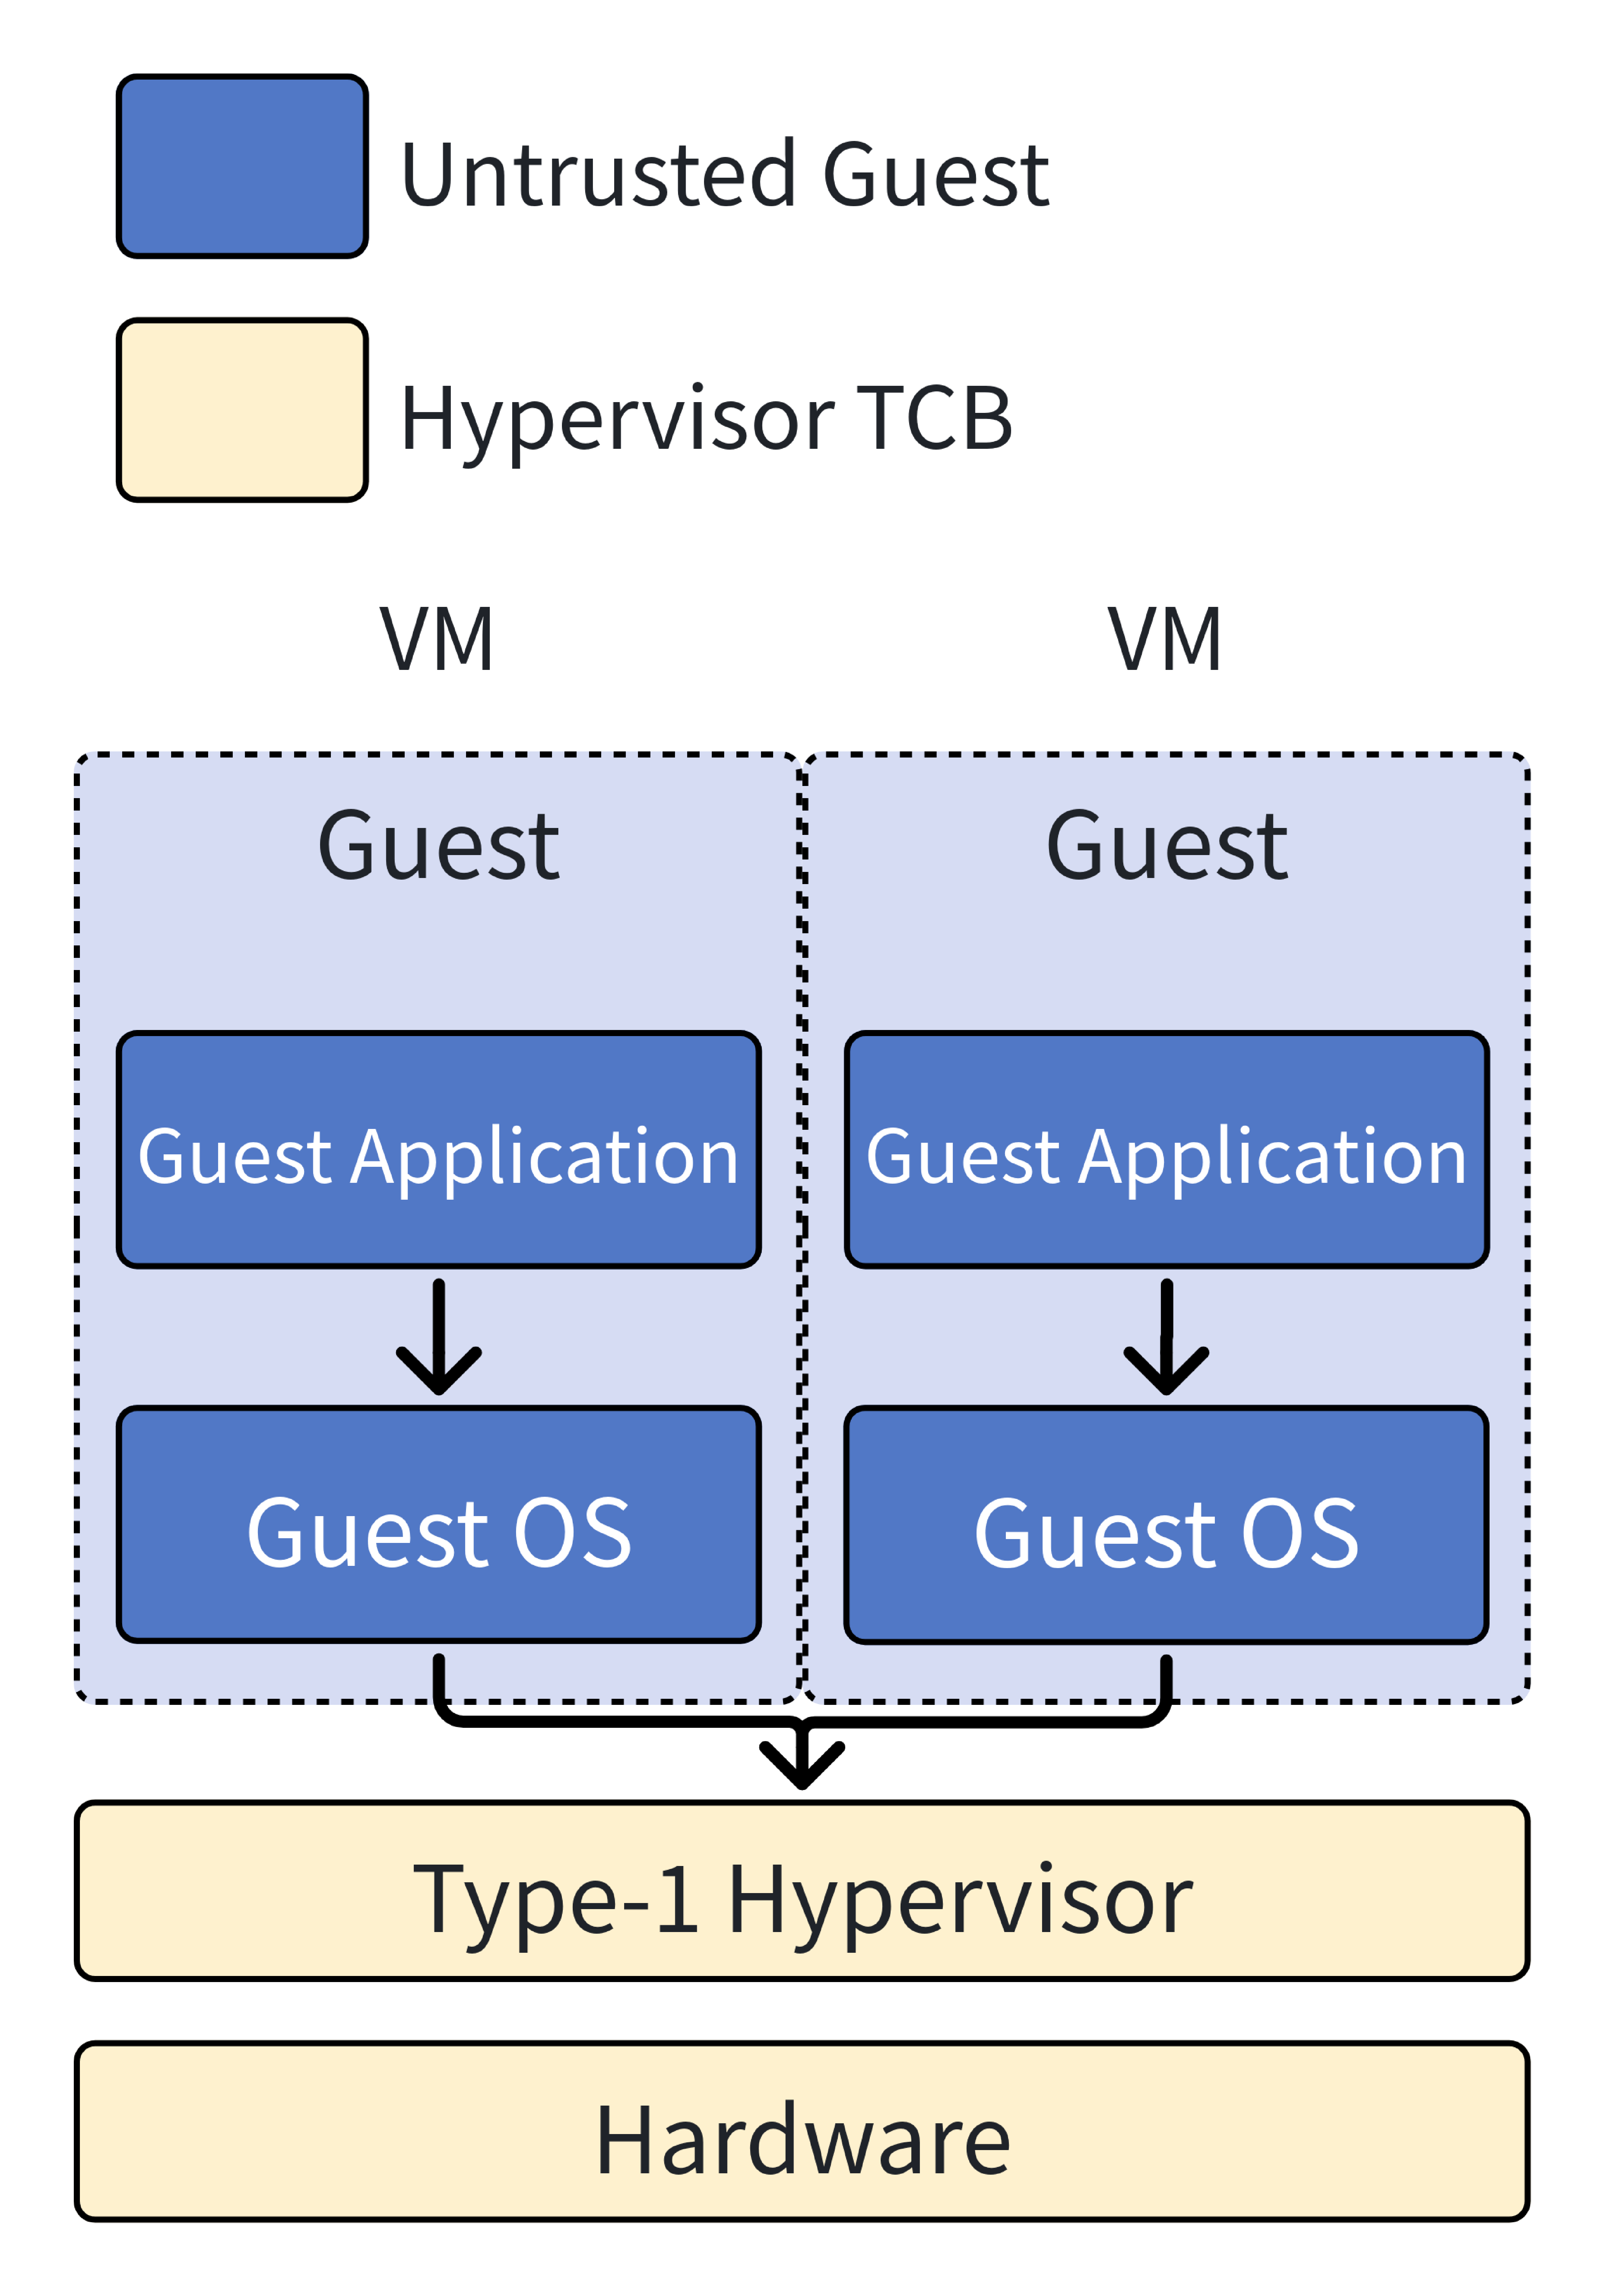
\includegraphics[width=0.3\linewidth]{type1_hyper.pdf}
			\label{type1_hyper}
		}
		\hfill
		\subfloat[]{
			\includegraphics[width=0.4\linewidth]{type2_hyper.pdf}
			\label{type2_hyper}
		}
		\caption{虚拟化技术分类}\label{hyper_style}
	\end{figure}
	
	根据Hypervisor与宿主环境的依赖关系，其部署架构可分为Type-1（裸金属型）与Type-2（宿主型）两类，如\ref{hyper_style}所示。Type-1架构直接运行于物理硬件之上，拥有对底层资源的绝对控制权，因其访存路径极短且指令处理链路精简，在性能表现与硬件利用率上占据显著优势。相比之下，Type-2架构寄生于宿主操作系统（Host OS），需跨越Host OS的抽象层间接访问硬件。尽管这种间接调用机制引入了额外的性能损耗，但其能够充分复用Host OS成熟的驱动体系与管理工具，展现出更强的环境适配性与部署灵活性。
	
	面向传统云服务场景的虚拟机监视器（如KVM\citess{kvm}、Xen\citess{xen}等）侧重于大规模租户的资源隔离。尽管已有研究尝试对其进行轻量化改造以向嵌入式场景迁移\citess{embedded-kvm,embedded-xen}，但受限于其宏内核架构下庞大的可信计算基（TCB），仍难以满足嵌入式环境对计算资源受限及严苛实时性的双重要求。为此，学术界与工业界相继提出了Bao、ACRN、XtratuM等针对高实时性与低功耗定制优化的轻量级方案\citess{bao,acrn,multipartes}。然而，此类方案在实际部署中仍面临资源动态调配率偏低及系统架构可扩展性受限等瓶颈。
	
	在车载与工业控制等高实时性关键场景中，基于微内核的虚拟化技术凭借其极简的特权层级与卓越的系统响应性能，成为突破上述瓶颈的优选路径。依托seL4微内核构建的CAmkES-VMM框架，通过极致的架构精简与低延迟设计，确立了高实时与低开销需求的理想范式\citess{sel4-virt}。同时，以QNX为代表的商用微内核方案，通过跨架构的强兼容性与关键任务（Mission-critical）调度策略，在自动驾驶等领域印证了微内核架构在兼顾强实时性与高安全性方面的固有优势\citess{qnx-Hypervisor}。
	
	综上所述，虚拟化技术已从早期的资源模拟演变为支撑现代复杂系统的核心基底。微内核虚拟化技术通过架构级的解耦与精简，在系统灵活性与执行效率之间取得了较好的平衡，契合现代嵌入式系统的复杂虚拟化需求，并已在严苛的实时性场景中确立了显著的技术优势地位。
	
	\subsection{虚拟化与TEE融合架构及演进现状}
	随着机密计算技术的不断发展，如何平衡执行环境的安全性、灵活性与生态兼容性成为了学术界与工业界关注的核心议题。根据系统对信任边界的划分及Enclave抽象级别的不同，现代隔离技术主要经历了纯虚拟化方案、基于应用/OS级抽象的TEE方案，以及基于机密虚拟机（CVM）抽象的软硬融合TEE方案三个演进阶段。
	
	\subsubsection{基于纯虚拟化TEE技术研究}
	主流指令集架构（ISA）均已引入成熟的硬件辅助虚拟化技术。传统的虚拟化技术侧重于资源复用与系统级隔离，使Hypervisor能够有效屏蔽底层异构硬件的差异。为提高系统的安全性，早期研究尝试通过极度精简Hypervisor或将其移出可信计算基（Trusted Computing Base, TCB）来构建安全隔离域。
	
	为优化Hypervisor自身的稳健性，Steinberg等人\citess{nova}借鉴微内核设计理念提出了NOVA架构。该方案将资源管理等逻辑移出特权内核，使核心代码缩减至约9KLoC，并为每个虚拟机分配用户态VMM实例以防范单点失效。Jia等人\citess{hyper-Enclave}提出的HyperEnclave架构则通过软件定义实现了与SGX兼容的Enclave抽象，成功将TEE保护能力与特定硬件微码解耦，并采用内存安全的Rust语言构建监视器。针对ARM架构，Pereira等人\citess{bao-Enclave}利用静态分区技术构建了Bao-Enclave，将安全功能从庞大的特权操作系统中剥离，实现了对硬件资源的精细化访问控制。
	
	基于纯虚拟化的方案凭借硬件平台的广泛兼容性，能够在不依赖特定安全微码的前提下实现基础的物理级隔离。然而，庞大的通用Hypervisor一旦被攻破，将直接威胁所有虚拟机的核心数据安全。即使是经过极度精简的轻量级Hypervisor，其作为特权层软件仍面临软件TCB冗余的问题，极易遭受复杂的侧信道分析，且难以防御针对物理内存的硬件探测攻击。纯虚拟化在底层硬件加密原语上的缺失，促使研究者转向架构级的硬件TEE方案。
	
	\subsubsection{基于进程与应用级抽象的细粒度TEE技术研究}
	为弥补纯虚拟化防御硬件攻击能力的不足，硬件厂商引入了具备芯片级内存加密与硬核隔离能力的专有扩展。早期架构级TEE主要聚焦于进程、应用或操作系统级别的细粒度抽象。这类方案仅将应用自身及必要的硬件纳入TCB，以换取极高的理论安全性。
	
	在x86架构中，Intel SGX（Software Guard Extensions）\citess{sgx}定义了极其严苛的威胁模型，假定包括OS与Hypervisor在内的所有系统软件栈均不可信。然而，由于传统可信应用（Trusted Application, TA）多采用C/C++构建，易受内存破坏攻击威胁（Wang等人\citess{rustsgx}虽提出Rust-SGX框架予以缓解，但仍需对代码进行深度重构）。更关键的是，SGX基于进程的隔离范式受限于受保护内存（EPC）容量与复杂的编程模型，导致深度学习等资源密集型应用面临巨大的迁移挑战。
	
	在嵌入式主导的ARM架构中，机密计算常以基于可信OS的TEE方案作为基础（例如基于ARM TrustZone扩展与GP-TEE\citess{gptee}规范的示例实现）。针对TrustZone安全世界资源独占的局限，Brasser等人\citess{sanctury}提出了SANCTUARY架构以动态划分用户态Enclave；Wang等人\citess{rt-tee}提出的RT-TEE确保了系统在遭遇拒绝服务（Denial of Service, DoS）攻击时的实时性；RusTEE\citess{rust-tz}则在编译阶段静态消除了TEE软件栈的内存隐患。
	
	在新兴的开源指令集方面，Keystone和Penglai是当前RISC-V主流的TEE方案。Penglai\citess{penglai,penglai-iopmp,penglai-hpmp}通过引入受护页表（GPT）等机制实现了高达512GB的动态隔离空间支持与高可扩展的I/O隔离，旨在解决云场景下的性能瓶颈；Keystone\citess{keystone}则引入了可编程的安全监视器，将核心功能模块化与可重用化。此外，Ozga等人\citess{ace}利用形式化验证框架确保了RISC-V TEE可信根的确定性。
	
	纯粹的TEE技术虽然提供了芯片级的强隔离，但基于进程或OS抽象的方案在适配复杂生态时面临极高的开发门槛。开发者必须手动剥离敏感代码以划分TCB、重写应用程序，或高度依赖特定的TEE-OS。这种架构不可避免地导致了严重的生态割裂，显著抬高了现有应用向机密计算环境迁移的综合成本。
	
	\subsubsection{基于机密虚拟机抽象的软硬融合TEE技术研究}
	为了彻底打破纯虚拟化在数据安全性上的瓶颈，同时解决应用/OS级TEE面临的开发门槛高与生态割裂困境，将虚拟化技术的灵活抽象能力与TEE专用安全指令拓展相互结合，成为了机密计算演进的必然选择。该范式提出了基于机密虚拟机（Confidential Virtual Machine, CVM）抽象的混合TEE架构。通过在硬件级加密的TEE中直接运行未经修改的Guest OS与大规模应用，最大程度地复用了现有操作系统生态，极大降低了厂商的开发与迁移成本。
	
	为破解灵活性与安全性的双重瓶颈，主流硬件厂商相继推出了支持CVM抽象的体系结构。以x86架构为例，AMD SEV\citess{sev}（Secure Encrypted Virtualization）利用硬件虚拟化扩展，为每个虚拟机分配唯一的地址空间标识符（ASID），并结合硬件级AES引擎确保内存数据以密文形式存储，实现了Guest VM与Hypervisor的语义脱钩；其增强版SEV-SNP\citess{sev-snp}则引入反向映射表（RMP）机制，强制防止Hypervisor篡改内存权限。Intel提出的TDX\citess{tdx}架构引入了全新的SEAM特权层级及专用模块，在架构层面彻底剥离了不可信Hypervisor对可信域生命周期的控制权。在ARM架构中，ARM CCA同样引入了机密领域（Realm）的概念，以支持虚拟机级别的硬件强隔离。
	
	与此同时，在开源的RISC-V生态中，传统多租户计算平台（Multi-tenant computing platforms）由于将平台固件、操作系统、虚拟机监视器及操作人员均纳入租户的可信计算基（TCB），导致其无法满足隐私导向型工作负载对TCB最小化的需求。针对这一局限性，Sahita等人\citess{cove}提出了面向RISC-V平台的机密虚拟机扩展（Confidential Virtual-Machine Extension, CoVE）架构的开源参考软件栈实现Salus。CoVE充分利用了RISC-V架构无历史包袱（Clean slate）的优势，定义了全新的指令集（ISA）与非指令集（Non-ISA）规范，以及系统级芯片（SoC）要求。该架构通过提供具备硬件认证（HW-attested）的TEE来实现对使用中数据（Data-in-use）的保护，为构建具备可量化TCB的原生机密计算架构奠定了基础。
	
	此外，机密计算不仅在隔离云端庞大的不可信代码中发挥着关键作用，更亟需向资源受限的嵌入式场景延伸。针对这一需求，Ozga等人\citess{ace}提出了面向嵌入式RISC-V系统的机密计算框架ACE（Assured Confidential Execution）。作为一种开源且免授权费（Royalty-free）的技术方案，ACE旨在将云端机密计算的安全能力下沉，以构建更安全、更可靠的任务关键型（Mission-critical）嵌入式系统，进一步完善了基于虚拟化扩展的RISC-V机密计算应用生态。
	
	综上所述，TEE架构的研究已从早期的纯软件隔离与进程级细粒度保护，全面转向兼顾高安全性与生态兼容性的虚拟机级保护，通过软硬协同的深度演进，逐步确立了现代机密计算的技术底座。
	
	\subsection{异构计算环境下GPU-TEE安全隔离与防护技术研究}
	
	随着端侧人工智能与云端大模型业务的爆发式增长，保障异构计算平台（如CPU+GPU/NPU）的数据隐私与模型完整性已成为系统安全领域的研究热点。在架构实现上，高性能服务器场景通常采用独立显存的离散式GPU，TEE仅需隔离GPU的内存映射I/O（MMIO）区域；而在端侧场景中，集成式硬件加速器通常与CPU共享物理内存，不仅需隔离MMIO，更要求对GPU缓冲区实施动态物理隔离。
	
	在基于CPU安全特性的监控机制研究中，Wu等人\citess{x86_gputee}提出的GEVisor利用现有Intel SGX构建了经过形式化验证的安全参考监视器。面向端侧统一内存架构，Deng等人\citess{arm_gputee}在StrongBox中利用ARM TrustZone技术，通过动态拦截MMIO与二阶段页表控制实现了高效隔离。为突破传统TEE频繁数据加解密导致的性能瓶颈，Fan等人\citess{x86_gputee1}提出的XpuTEE框架引入微型监控器XM，通过联合抽象与直接物理映射实现了“去加密化”监控，将大模型推理开销显著压缩至2.5\%以下。
	
	为应对新一代指令集架构与存量基础设施的兼容性挑战，机密计算研究逐渐转向软硬协同的深度解耦范式。Wang等人\citess{cage}提出的CAGE框架借助粒度保护检查（GPC）原语率先实现了ARMv9架构下的GPU硬件级隔离。此外，针对现有机密加速器高度依赖特定硬件更迭的问题，Wang等人\citess{ccai}设计了具备强兼容性的ccAI系统。该方案在物理层动态截获并重定向GPU任务提交路径，平滑支持了DeepSeek、Llama等大模型的机密推理。
	
	尽管异构隔离技术不断演进，Lu等人\citess{gpu_sec}在MOLE研究中揭示了新型硬件侧攻击面：GPU内部集成的微控制器（MCU，如Falcon/GSP）拥有超越系统IOMMU限制的特权级访问能力。攻击者可通过劫持MCU固件绕过CPU侧监控机制直接窃取TEE显存数据。该发现打破了直通即安全的传统假设，表明未来的异构机密计算亟需建立涵盖外设内部组件完整性度量的全路径防护体系。
	
	\section{本文主要贡献和创新}
	本文以基于RISC-V硬件虚拟化扩展及机密虚拟机（CVM）安全生命周期管理为核心研究对象。为了克服传统虚拟化在机密计算场景中的安全隔离瓶颈，本文依托既有的基于微内核的虚拟化方案EasyAda-Hypervisor，重点开展了底层安全固件设计、虚拟化组件安全扩展及端侧异构机密计算环境的构建。其主要研究内容与创新工作如下：
	
	1.提出并实现了一种基于Rust内存安全特性的模块化底层安全监视器EasyAda-SM：针对传统C语言构建的安全固件极易受内存破坏漏洞威胁的局限性，本文采用Rust语言从底层独立设计并实现了EasyAda-SM。在架构抽象层面，构建了安全区域与内存管理层，并深度结合Rust的所有权模型，实现了一套基于页分配器（Page Allocator）的安全内存调度机制，从而在编译期静态消除了二次释放等内存隐患。更进一步，为了实现执行环境间的强隔离，本文将CPU和设备侧物理内存保护机制抽象为统一的内存保护原语，严格切断了不可信软硬件对CVM安全内存的物理级访问路径。由此可见，该设计从软件自身安全性与硬件物理隔离两个维度，为整个系统确立了坚实的信任根基。
	
	2.提出并实现基于微内核的可信虚拟化方案EasyAda-trust：为适应机密计算的严苛安全需求，本文对现有的EasyAda-Hypervisor进行了深度的安全扩展与架构增强。具体而言，在资源调度方面，本文引入了职责解耦机制，将常规的物理内存分配与设备发现保留在不可信的Hypervisor层，而将二阶段页表隔离映射、安全区域动态构建及可信上下文切换等核心敏感操作全权委托给EasyAda-SM处理。此外，在运行态安全防护方面，结合本文设计的基于本地证明机制的安全启动链与机密执行流，确保了CVM的CPU上下文及内存视图对Hypervisor的绝对隐匿。基于上述软硬协同的设计，本文在不破坏原有微内核架构的前提下，成功实现了不可信虚拟机与机密虚拟机的安全共存与统一调度。
	
	3.扩展EasyAda-trust架构并构建端侧机密异构计算环境：针对端侧异构硬件中支持直接内存访问（DMA）的外设可能绕过CPU隔离机制发起的恶意攻击，本文进一步扩展了EasyAda-trust的系统设计。首先在硬件防护层，通过引入RISC-V I/O物理内存保护（IOPMP）扩展，实现了基于设备唯一标识（SID）的外设动态鉴权与细粒度内存访问控制。然而，仅依靠底层硬件隔离难以满足复杂外设在多执行环境间的动态调度需求；因此在此基础上，本文创新性地提出并构建了专用的加速器管理CVM代理架构。该架构利用I/O半虚拟化技术与安全共享内存映射机制，在严格保障用户AI模型权重及隐私数据机密性与完整性的前提下，成功实现了底层硬件加速器在不可信与机密执行环境间的时空复用。值得注意的是，这一系列设计不仅化解了跨域DMA攻击威胁，更为端侧异构算力的泛化安全部署确立了完备的技术范式。
	
	\section{论文结构}
	本文的内容组织与结构安排如下：
	
	第一章：绪论。首先详细阐述了智能物联网与端侧异构计算环境下面临的安全性挑战，进而深入探讨了当前底层固件与虚拟化隔离所面临的核心痛点与科学问题。针对上述问题，引出了基于开放指令集与微内核架构构建可信执行环境的研究背景和意义，最后概述了本文的主要研究内容与章节结构安排。
	
	第二章：相关技术理论概述。为解决第一章提出的架构痛点，本章重点探讨了本文方案所依赖的底层技术底座。首先，详细阐述了底层硬件隔离机制的相关概念（包括特权级模型、物理内存保护体系及硬件虚拟化扩展）；其次，介绍了机密计算的演进范式，并深入探讨了微内核虚拟化的相关理论；最后，进一步说明了异构计算场景下信任边界延伸的架构兼容性需求，从而为后续的系统设计奠定理论基础。
	
	第三章：基于RISC-V的微内核虚拟化方案设计。本章从宏观层面介绍了在端侧强隔离需求下如何精准界定系统可信计算基（Trusted Computing Base，TCB）边界。基于该信任边界，阐述了安全启动、内存隔离与中断路由等多维防护机制的构建思路。值得注意的是，本章最后对基于动态外设隔离的硬件加速器安全复用模型进行了具体说明，从全局视角确立了系统的架构蓝图。
	
	第四章：内存安全的模块化安全监视器实现。本章详细阐述了针对最高特权级固件内存脆弱性的防护机制。具体而言，首先探讨了如何从语言层面消除内存破坏漏洞，随后介绍了细粒度安全区域管理的抽象方法。此外，本章还对机密上下文切换、信任链推演及外设安全授权的理论模型进行了深入探讨，旨在筑牢系统的底层信任根。
	
	第五章：基于微内核的可信虚拟化方案实现。本章介绍了CPU状态隐匿与内存管控解耦的具体集成方案。为了应对复杂的I/O安全威胁，进一步阐述了防DMA攻击与端到端数据保护的部署流程。最后，对跨域通信信道与加速器机密部署机制进行了具体说明，由此打通了微内核机密虚拟化的全链路技术栈。
	
	第六章：系统测试与分析。为验证上述架构设计与系统集成的有效性，本章介绍了多维度定量评估与安全分析体系的构建方法。在性能评估方面，通过基准测试量化了底层固件的生态兼容性与计算开销；在安全验证方面，设计边界条件检验了双向证明与可信启动链的稳健性。基于上述结果，对系统在安全隔离与执行效能间的架构折中进行了全面评估，充分证明了本文方案在实际嵌入式场景中的可行性。
	
	第七章：总结与展望。综合前述理论、设计与实验验证，对本文的研究工作与核心理论贡献进行系统性总结。同时，客观审视了目前微内核架构与底层安全机制融合中存在的局限性，并由此提出多核并发调度优化、核心组件形式化验证及异构总线安全等后续的研究方向。
	
	
	\chapter{相关技术理论概论}
	\section{RISC-V背景知识}
	x86架构因其漫长的发展历史与向后兼容性负担，指令集日趋复杂庞大。尽管在服务器等高性能计算领域表现良好，却难以契合嵌入式场景对严苛功耗与成本的约束。
	
	ARM架构作为精简指令集（RISC）的代表，凭借IP授权模式赋予下游厂商一定的定制自由度，在嵌入式市场占据主导地位。然而，受限于其封闭的商业壁垒，硬件开发面临高昂的IP授权成本；同时，ARM架构跨代演进（如ARMv7至ARMv8）差异显著，导致了严重的指令集碎片化问题，系统高度依赖特定版本的编译工具链以维持跨平台兼容性与性能优化。
	
	相比之下，新兴的RISC-V架构凭借开源开放与高度模块化的设计理念，与系统软件的解耦演进需求高度契合。硬件厂商可根据具体场景按需组合指令集扩展，软件生态亦能据此实现灵活伸缩，有效规避了跨代架构更迭带来的高昂代码移植成本。在云边端协同计算趋势下，资源受限的边缘节点可仅实现基础指令子集以满足极低功耗约束，而云端高性能设备则可集成复杂扩展以跃升算力。RISC-V这种高度弹性的架构特性，为构建跨越异构硬件的通用、可扩展的可信执行环境（TEE）提供了理想的底层硬件支撑。

	\subsection{RISC-V特权级介绍}
	\begin{figure}[!htb]
		\centering
		\subfloat[特权级转换]{
			\includegraphics[width=0.45\linewidth]{priv_nonvirt.pdf}
			\label{priv_nonvirt}
		}
		\hfill
		\subfloat[软硬件架构]{
			\includegraphics[width=0.5\linewidth]{overall_nonvirt_arch.pdf}
			\label{overall_nonvirt_arch}
		}
		\caption{未引入硬件虚拟化扩展时RISC-V系统架构}\label{overall_nonvirt}
	\end{figure}
	RISC-V架构将独立的CPU核心抽象为硬件线程（Hard Thread，hart）。在任何运行时态下，hart均处于特定的特权级中。RISC-V规范定义了由低至高的三种主要特权级：用户模式（U-Mode）、监管者模式（S-Mode）与机器模式（M-Mode）。如图\ref{overall_nonvirt_arch}所示，根据指令集标准，M态为强制实现的基础特权级，而U态与S态为可选扩展。实际商用硬件通常基于特定应用场景与功耗考量进行架构裁剪，如运行RTOS或裸机应用的MCU场景可以仅实现U态和M态，甚至仅实现单M态。
	
	各特权级之间具备严格的权限隔离边界\citess{rv-setman}：U-Mode作为最低特权级，仅获准访问通用寄存器并执行基础指令，其访存操作严格受限于页表映射机制；S-Mode在此基础上，进一步获准访问特定的控制与状态寄存器（Control Status Register，CSR）并执行相关特权指令，其访存操作同样受限于MMU页表机制；M态作为系统最高特权级，拥有对所有物理硬件、CSR及特权指令的无限制访问权，并可绕过页表直接寻址物理内存。任何低特权级尝试执行越权指令的行为均会触发硬件异常拦截。
	
	在特权级状态转换机制上，系统上电重置时hart默认初始化为M态。控制流从高特权级向低特权级转移需显式执行mret或sret指令完成状态降级；反之，当系统发生外部中断或执行异常时，硬件将根据CSR中的委派（Delegation）配置，自动陷入（Trap）至S态或M态的异常向量入口。此外，低特权级软件可主动触发ecall或ebreak指令发起系统调用，以同步陷入的方式将控制权安全移交至高特权级执行环境。各特权级间的状态转换逻辑如图\ref{priv_nonvirt}所示。

	\subsection{RISC-V中断与异常处理机制介绍}
	RISC-V架构将所有打破正常程序控制流的突发事件统称为陷入（Trap）。在微架构层面，陷入被严格划分为两类：同步的异常（Exception）与异步的中断（Interrupt）。异常通常由当前执行的指令直接引发（如非法指令解码、缺页异常或主动发起的ecall系统调用），而中断则由独立于当前执行流的外部异步事件触发。RISC-V手册规定中断按类型分为外部中断（External Interrupt）、软件中断（Software Interrupt）、时钟中断（Timer Interrupt）三种。
	
	根据RISC-V基础特权级规范，系统发生的所有陷入默认均强制路由至最高特权级M态处理。然而，在部署了复杂操作系统或Hypervisor的场景中，频繁的M态陷入与上下文切换将引入不可接受的性能开销。为此，RISC-V创新性地设计了陷入委派机制。通过精细化配置M态异常委派寄存器（medeleg）与中断委派寄存器（mideleg），底层安全固件可将特定类型的陷入事件（如S态下的缺页异常或时钟中断）显式旁路，使其直接触发S态的陷入响应而无需M态介入。这一机制极大地缩短了关键中断的响应延迟，是实现高效软硬件协同与机密虚拟化资源调度的核心架构支撑。
	
	
	\subsection{RISC-V内存保护机制介绍}
	\subsubsection{物理内存保护（PMP）机制}
	物理内存保护（Physical Memory Protection，PMP）机制是RISC-V架构标准提供的核心安全原语，也是在该架构上构建TEE的必要底层硬件支撑。在微架构层面，每个hart均集成了一组专用的PMP地址寄存器（pmpaddrx）与配置寄存器（pmpcfgx），且这些寄存器的读写权限被严格限制在M态。
	
	在使能了PMP机制的硬件平台中，系统默认采用严格的隔离访问策略：在未显式授权的情况下，运行在更低特权级的软件被默认限制对任何物理地址的访问。通过在M态下对PMP寄存器组进行精细化配置，系统能够以hart为粒度，为其划分特定的连续物理地址空间，并显式授予相应的读、写及执行权限。简言之，PMP机制从硬件底层提供了一种强隔离的访问控制手段，能够精准限制特定hart对任意物理内存区域的访存边界与操作能力。
	
	\subsubsection{增强的物理内存保护（Smepmp）机制}
	Smepmp（Supervisor Mode Execution Prevention and Machine-mode Physical Memory Protection）扩展是对RISC-V基础PMP机制的关键安全增强。在原生PMP架构中，锁定位（L位）的语义存在天然的耦合局限：当L=0时，M态默认拥有对全量物理内存的无限制访问权；当L=1时，M态与低特权级将被强制绑定相同的R/W/X权限。这种粗粒度的设计导致系统无法在赋予S态合法访存权限的同时有效剥夺M态的对应权限，难以防御针对高特权级固件的混淆代理（Confused Deputy）攻击，亦无法从架构层面彻底杜绝M态意外执行驻留于低特权级内存中的恶意载荷。
	
	为突破上述架构瓶颈，Smepmp扩展创新性地引入了机器安全配置寄存器（mseccfg）。该寄存器通过三个核心控制位重塑了底层的物理访存控制逻辑：首先是机器模式锁定（MML）位，当MML被置位时，系统将彻底重载传统PMP配置中L位与R/W/X位的组合语义，实现了M态与更低特权级内存权限的深度解耦。例如系统可配置仅低特权级可读写、M态不可访问的隔离区域，从而在物理硬件层面严格贯彻了最小特权原则。其次是机器模式白名单策略（MMWP）位，使能该位将逆转M态的默认访存行为，从原有的默认放行切换为严苛的默认拒绝（Default-Deny），强制要求M态的所有访存操作必须命中显式授权的PMP条目。最后是规则锁定旁路（RLB）位，它在维持整体隔离强度的前提下，允许授权的安全固件动态修改已锁定的PMP条目，极大提升了TEE运行时的内存管理弹性。
	
	综上所述，Smepmp机制在微架构层面弥补了原生PMP权限颗粒度粗糙的设计缺陷，而原生PMP机制以最小的硬件开销构筑了坚实的宏观物理隔离边界，为嵌入式环境提供了兼具高实时性与高性价比的底层安全原语。
	
	\subsubsection{I/O物理内存保护（IOPMP）机制}
	输入输出物理内存保护（Input/Output Physical Memory Protection，IOPMP）是RISC-V架构中用于保障系统级外设访存安全的关键硬件扩展。尽管原生的PMP机制能够有效限制hart的越权访存行为，但它仅作用于CPU侧，无法约束具备DMA能力的外设。恶意或受控的外设可轻易绕过CPU的PMP隔离边界，直接对受保护的物理内存发起读取或篡改操作（即DMA攻击），这构成了机密计算环境下的重大安全隐患。
	
	为弥补这一架构级安全短板，RISC-V引入了IOPMP扩展。在微架构实现上，IOPMP通常部署于系统互连总线与外设控制器之间，充当所有I/O访存事务的硬件级安全网关。其核心访问控制逻辑基于设备唯一标识（Source ID，SID）展开：当外设发起总线级读写请求时，IOPMP会首先捕获该请求携带的SID，并通过内部的路由表将其映射至特定的内存域（Memory Domain，MD）。每个内存域内配置了一组类似于PMP的规则条目，用于精确界定该SID对应的设备所能访问的连续物理地址范围及其读写权限。任何未命中授权条目的DMA请求均会被IOPMP硬件直接拦截并上报异常。
	
	\subsection{RISC-V硬件虚拟化扩展（H-extension）介绍}
	\begin{figure}[!htb]
		\centering
		\subfloat[特权级转换]{
			\includegraphics[width=0.6\linewidth]{priv_virt.pdf}
			\label{priv_virt}
		}
		\hfill
		\subfloat[软硬件架构]{
			\includegraphics[width=0.7\linewidth]{overall_virt_arch.pdf}
			\label{overall_virt_arch}
		}
		\caption{引入硬件虚拟化扩展后的RISC-V系统架构}\label{overall_virt}
	\end{figure}
	RISC-V硬件虚拟化扩展（H-extension）是RISC-V指令集架构中专为提升Hypervisor运行效率而设计的关键硬件扩展。传统软件模拟的虚拟化方案面临高昂的陷入-模拟开销，而H扩展通过在处理器微架构层面引入新的特权级、寄存器副本以及二阶段地址翻译机制，从硬件底层为高效构建Type-1或Type-2型Hypervisor提供了系统级支撑。
	
	如图\ref{overall_virt}所示，使能H扩展后，原有的S态被扩展为Hypervisor扩展监管者模式（HS-Mode），同时新增了虚拟监管者模式（VS-Mode）与虚拟用户模式（VU-Mode）。在HS态下运行的Hypervisor拥有对物理硬件与虚拟机的完全控制权；而Guest OS及Guest App则分别运行在VS态与VU态下。这种设计确保了Guest OS无需修改核心代码即可无感运行，并在试图执行影响全局的敏感特权指令时安全地触发硬件异常并陷入HS态处理。
	
	频繁的虚拟机退出（VM-Exit）是制约虚拟化性能的核心瓶颈之一。为此，H扩展为VS态引入了一套完整的S态寄存器影子副本（如vsstatus、vstvec、vsepc、vsscratch等）。当处理器运行在虚拟化环境（V=1）时，Guest OS对常规S态寄存器的读写操作会被硬件自动重定向至对应的虚拟控制状态寄存器中。这一机制使得客户系统在配置自身上下文时无需陷入HS态，极大地降低了寄存器访问带来的上下文切换开销。
	
	为实现虚拟机间的物理内存强隔离，H扩展引入了二阶段页表机制。第一阶段（Stage-1）完全由Guest OS控制，负责将虚拟地址（VA）翻译为客户物理地址（GPA），其页表基址由虚拟监管者地址转换与保护寄存器（vsatp）管理；第二阶段（Stage-2）由Hypervisor严密管控，负责将GPA强制翻译为真实的宿主物理地址（HPA），其页表基址由Hypervisor客户地址转换与保护寄存器（hgatp）管理。MMU在处理VS/VU-Mode的访存请求时，会自动串行执行这两阶翻译，彻底阻断了虚拟机越权访问宿主物理内存或其他虚拟机地址空间的可能。
	
	同时，H扩展增强了RISC-V原有的委派机制。通过配置Hypervisor级的中断与异常委派寄存器（hideleg与hedeleg），系统可将原本默认陷入HS态的特定异常（如VS态系统调用或缺页异常）直接旁路委派至VS态，交由Guest OS内部的处理程序直接响应。此外，H扩展设计了完善的虚拟中断注入机制（如通过hvip寄存器配置VSSIP、VSTIP、VSEIP），允许Hypervisor在软件层面灵活模拟虚拟硬件外设，并高效地向目标VS态挂起并注入虚拟中断信号。
	
	\section{可信执行环境（TEE）相关技术介绍}
	\begin{figure}[!htb]
		\centering
		\subfloat[可信应用]{
			\includegraphics[width=0.45\linewidth]{tee_app.pdf}
			\label{tee_app}
		}
		\hfill
		\subfloat[可信操作系统]{
			\includegraphics[width=0.5\linewidth]{tee_os.pdf}
			\label{tee_os}
		}
		\subfloat[机密虚拟机]{
			\includegraphics[width=0.5\linewidth]{tee_vm.pdf}
			\label{tee_vm}
		}
		\caption{基于系统抽象层级与软件执行模型的TEE分类}\label{tee_style}
	\end{figure}
	TEE通过在硬件微架构层面构建受保护的隔离执行空间，通过对传入和传出的数据进行加密，为敏感代码与执行状态确立了系统级的机密性与完整性保障。尤为关键的是，TEE能够从指令集架构底层重塑信任边界，有效抵御来自系统中任何潜在恶意实体或高特权级系统软件（如不可信的宿主操作系统内核或虚拟机监视器）的越权访问与潜在攻击。相较于全同态加密或多方安全计算等纯密码学计算范式，TEE凭借以下三大核心特性展现出显著的技术实用性与工程优势\citess{tee_survey}：
	
	1.\textbf{通用可编程性（General Purpose Computation）}：TEE内部所支持的执行功能通常表现为用户自定义程序，这赋予了其图灵完备的通用计算能力，使其能够广泛适配各类复杂的业务功能与算法形态。
	
	2.\textbf{强机密性与执行完整性（Integrity and Privacy）}：TEE在物理信任边界内同时提供双重安全属性。机密性（Confidentiality）\citess{cc_def}确保了外部潜在攻击者无法从计算过程中窥探或获取任何敏感信息，而完整性（Integrity）则从底层机制上保证了目标程序的执行逻辑免遭篡改并被严格且正确地执行。
	
	3.\textbf{近似原生的计算性能（High Performance）}：TEE的核心计算范式是在安全飞地内部将所有加密输入解密后，直接依托物理CPU在明文状态下执行目标自定义程序。因此，除了处理加密数据输入输出所产生的额外开销外，TEE能够充分释放并利用CPU的原生运算速度，彻底规避了纯密码学方案中高昂的算力惩罚，具备极高的高性能优势。
	
	根据系统抽象层级与软件执行模型的差异，如图\ref{tee_style}所示，当前业界的隔离与机密计算架构主要经历了以下三种演进范式：
	
	1.基于纯虚拟化的安全隔离方案：传统的纯虚拟化方案（如基于KVM或Xen的隔离）通过Hypervisor在系统级提供虚拟机间的强隔离。然而，这种方案的安全性高度依赖于Hypervisor自身的代码可靠性。由于通用Hypervisor体量庞大且极其复杂，其作为可信计算基（TCB）存在巨大的攻击面。一旦Hypervisor被攻破，所有虚拟机的核心数据将面临严重威胁；且纯虚拟化缺乏底层硬件密码学机制的支撑，难以抵御物理层面的硬件探测与内存窃取攻击。这种安全性的内生不足，促使业界向具备芯片级强隔离的TEE技术演进。
	
	2.面向可信操作系统（Trusted OS）的TEE架构:早期硬件辅助的TEE架构主要聚焦于细粒度的可信应用（TA）或可信操作系统（TOS）级别的抽象。此类方案的典型代表包括面向应用级抽象的Intel SGX。在基于可信OS的架构中，通常引入定制化的系统来调度多个TA（例如基于ARM TrustZone扩展与GP-TEE规范的示例实现）。Keystone和Penglai是当前RISC-V主流的TEE方案，它们分别探索了灵活的应用级与OS级隔离机制。这类方案虽然弥补了纯虚拟化的安全性短板，提供了芯片级的强隔离与内存保护，但存在显著的局限性：开发者必须手动剥离敏感代码以划分TCB、重写应用程序或高度依赖特定的专属TEE-OS。这种极高的开发门槛不可避免地导致了严重的生态割裂，显著抬高了现有庞大应用向机密计算环境平滑迁移的综合成本。
	
	3.面向机密虚拟机（Confidential VM）的TEE架构:为了彻底打破纯虚拟化在数据安全性上的瓶颈，同时解决基于应用/OS级TEE面临的生态割裂与开发门槛高的困境，将虚拟化技术的灵活抽象能力与TEE专用的硬件安全指令拓展相互结合，成为了机密计算演进的必然选择。该范式提出了基于机密虚拟机（CVM）抽象的混合TEE架构（如Intel TDX、AMD SEV-SNP、ARM CCA以及RISC-V架构下的机密虚拟机扩展CoVE等）。通过将复杂的Hypervisor移出TCB，并在硬件级加密的TEE中直接运行未经修改的Guest OS与大规模应用，该架构最大程度地复用了现有的操作系统生态。这不仅有效收敛了TCB的攻击面，还极大降低了厂商的开发与应用迁移成本，代表了当前机密计算的最前沿趋势。
	
	\subsection{面向异构计算环境的TEE}
	业界已经在CPU侧建立起了相对成熟的TEE机制用于隔离和保护敏感数据。然而，随着机器学习、大数据处理等数据密集型应用的爆发，单核或多核CPU的算力已无法满足海量数据的高性能计算需求。为了在利用GPU、NPU和FPGA等硬件加速器提供澎湃算力的同时，依然能够享受高强度的机密性、完整性与隔离性保护，将TEE的安全信任边界从主机CPU延伸至异构加速器设备（即构建加速器TEE或异构TEE）成为了学术界与工业界的必然演进方向。这种信任边界的延伸不仅需要保护传统的明文数据和代码，还必须涵盖AI模型参数、输入输出特征、页表映射以及底层硬件环境状态。
	
	根据加速器与主机CPU在物理架构与互连方式上的差异，当前异构计算环境的集成范式主要可划分为以下三类。不同的范式对底层安全隔离机制与TEE架构设计提出了截然不同的挑战：

	1.指令集扩展（ISA Extension）：该范式将AI或密码学运算逻辑直接嵌入CPU的执行流水线中，通过RISC-V等架构预留的编码空间实现自定义指令扩展（如矩阵运算或向量增强）。加速单元共享处理器的通用寄存器组或向量寄存器，加速指令由CPU译码后直接分发至执行单元。此模式消除了数据在异构组件间的移动开销，具有极高的指令响应速度和极低的上下文切换延迟。在TEE视角下，其信任边界完全收敛在CPU物理核心内部，复用原生的CPU特权级与内存隔离机制即可实现高安全性的保护。它适用于细粒度、高频次的张量运算，是追求极致单核计算密度及实时性场景的首选理论模型。
		
	2.片上协处理器（On-chip Coprocessor）：此范式下，加速器作为SoC内部独立的硬件IP存在，通过片上系统总线与CPU交互。加速器拥有独立的控制逻辑与局部存储空间，由CPU通过内存映射I/O（MMIO）进行任务配置和启动，并通过DMA自主完成大规模数据的搬运。通过异步工作机制，CPU仅负责高层调度，而加速器专注于流水化处理大体量数据。从安全维度来看，协处理器通常与CPU共享片上物理内存，其TEE设计需重点防范恶意的越权DMA攻击，高度依赖诸如IOPMP等总线级物理内存保护硬件来确立硬件级隔离边界。这种模式在能效比与系统灵活性之间进行了平衡，是当前主流嵌入式AI SoC的硬件范式。
		
	3.片外独立加速器（Discrete Accelerator）：加速器位于独立的物理芯片或插卡上，通过高速串行总线（如PCIe或CXL）与主机互联。此类加速器通常具备独立的高带宽全局显存（如HBM/GDDR）和复杂的层次化缓存结构。系统通过驱动程序管理设备内存空间，并采用命令队列模式进行大规模任务的批处理提交。其逻辑设计的复杂度不再受限于主机SoC的热设计功耗与封装面积，能够提供极高的峰值算力。然而在机密计算场景中，由于跨物理总线通信的存在，该范式不仅对主机侧的安全隔离机制提出了更高的时延容忍度要求，还必须引入端到端的内存加密引擎（MEE）与总线加密协议（如TDISP），以彻底抵御总线探测、数据篡改与物理重放攻击。

	尽管异构TEE研究在近年来呈现出爆发式增长，但其在真实物理设备上的大规模部署仍面临严峻的工程与理论痛点。首先是系统架构的碎片化与通用性缺失，现存的大量加速器TEE方案往往强绑定于特定的“CPU-加速器”硬件组合，缺乏标准化的软硬件交互抽象，导致跨平台迁移极其困难。其次是可信计算基的急剧膨胀，为了支持复杂的异构加速器调度，传统方案往往被迫将体量庞大的设备驱动程序（如动辄百万行代码的GPU软件栈）直接纳入可信环境中，严重违背了安全固件微内核化的极简设计初衷，极大地增加了系统的潜在攻击面。

	\section{微内核相关知识介绍}
	\subsection{微内核操作系统EasyAda介绍}

	EasyAda是一款自研微内核操作系统，如图\ref{mk_arch}所示，其设计理念遵循最小特权原则，旨在构建高安全性、高可靠性的操作系统内核，适用于对稳定性和安全性要求较高的嵌入式应用场景。
	\begin{figure}[!h]
		\centering
		\includegraphics[width=1\linewidth]{microkernel.pdf}
		\caption{微内核操作系统EasyAda总体架构}
		\label{mk_arch}
	\end{figure}
	EasyAda将内核态精简为仅保留必要的特权功能模块，如核间通信、权能管理、中断与异常处理、时钟管理、地址空间管理和内核对象管理等核心组件，内核将对外提供的服务封装为系统调用接口，仅暴露较小的攻击面。同时，通过硬件抽象层（Hardware Abstraction Layer，HAL）抽象了操作系统依赖的硬件原语，如启动/暂停CPU核心，中断配置和处理，MMU配置等，实现了统一的硬件操作接口。这降低了操作系统在不同指令集和架构间移植的难度，并且有效降低了内核代码的复杂度，确保EasyAda可以在异构环境上对外提供统一的软件平台。
	
	EasyAda将除核心功能外的其余大部分服务迁移至用户态，在地址空间隔离的上下文中运行，并由根服务（Rootserver）统一管理。根服务作为一个运行在用户态的多线程进程，集成了多个功能子系统。这些子系统既包括独立的模块化组件，如文件系统、进程管理、网络协议栈等，也包括执行特定任务的独立线程，如Shell交互模块等。根服务将对外提供的服务封装为RPC接口，为操作系统提供统一、透明的服务访问接口，并且对RPC参数进行严格的检查以防范外部攻击。其他服务或用户应用可以通过系统共享库提供的POSIX API前端，将函数调用转换为RPC调用。同时，所有应用和系统服务均拥有独立的权能空间，仅能访问当前权能空间支持的RPC接口和系统调用，进一步缩小了系统的攻击面。
	
	基于微内核的设计思想，EasyAda相比Linux等宏内核操作系统具备更小的软件TCB，而相比传统的RTOS如FreeRTOS等，EasyAda又具备强大的可扩展性，可以通过扩展系统服务实现与宏内核对等的功能和性能。因此EasyAda通过灵活调整用户态系统服务配置，可以适应从边缘到中高端嵌入式等多维度的场景和需求，为云边端场景提供通用的OS底座。
	
	由于EasyAda被设计为面向多样化场景的通用操作系统，因此其应用和系统服务运行在用户态，内核运行在内核态（未开启虚拟化）或Hypervisor态（开启虚拟化支持），并且通过安全固件接口与运行在最高特权级的安全固件进行交互以实现硬件管理。

	\subsection{微内核虚拟化方案EasyAda-Hypervisor介绍}
	图\ref{hyper_arch}展示了支持管理CVM生命周期的、基于RISC-V的EasyAda-Hypervisor设计。EasyAda-Hypervisor严格遵守了EasyAda微内核的设计哲学和思路：
	\begin{figure}[!h]
		\centering
		\includegraphics[width=1\linewidth]{Hypervisor.pdf}
		\caption{EasyAda-Hypervisor总体架构}
		\label{hyper_arch}
	\end{figure}

	1.统一资源管理：主要系统资源由EasyAda负责管理和分配。充分复用微内核操作系统现有代码和能力，实现统一的资源管理并减少EasyAda-Hypervisor的代码量，缩小其TCB。
	
	2.Hypervisor解耦：Hypervisor被划分为运行在EasyAda用户态下的VMM和内核态下的Hypervisor驱动，以尽可能复用EasyAda现有代码和功能。前者负责主要的VM管理工作，包括管理VM生命周期和软硬件资源，模拟虚拟化设备后端，以及管理VM服务线程等；后者作为屏蔽不同架构硬件虚拟化扩展实现的抽象层，对外提供基于虚拟化硬件原语抽象的统一接口，完成对硬件虚拟化扩展相关寄存器的配置，以及接收和处理VM中断和异常等。
	
	3.静态分区：Hypervisor采用静态分区策略。虽然该策略在资源动态调配上略显不足，但考虑到嵌入式场景应用高度定制化、负载相对确定的特点，静态分区策略足以满足其功能需求。更为关键的是，静态分区策略可以简化代码逻辑，缩小Hypervisor的攻击面。这一点在引入CVM支持之后更加重要，因为标准RISC-V CoVE扩展要求SM实现数十个SBI接口以实现对CVM资源的细粒度控制，这不仅显著增大了TCB的攻击面，还导致Hypervisor需要多次SBI调用才能完成单一功能，严重影响了系统的实时性和性能。
	
	EasyAda-Hypervisor通过在EasyAda中引入两个核心组件实现基于硬件虚拟化扩展的VM生命周期管理。其中，运行在Hypervisor态的Hypervisor驱动负责抽象虚拟化硬件原语并对上提供虚拟化能力接口。其虚拟化能力主要可以分为以下五类：（1）CPU虚拟化：基于虚拟特权级为VM提供符合其运行要求数量的vCPU，并在隔离的硬件环境中运行VM上下文，在实现操作系统无感迁移运行的同时，避免VM访问和篡改Hypervisor或其他VM的上下文信息；（2）内存虚拟化：基于硬件虚拟化提供的二阶段地址翻译能力，通过动态配置和管理VM的二阶段页表，实现细粒度的、VM无感的强制内存隔离；（3） 中断虚拟化：基于硬件提供的中断控制器，通过中断注入或中断直通等手段实现VM中断管理，避免VM接收和配置不属于当前VM的中断；（4）时钟虚拟化：基于虚拟硬件时钟，通过虚拟化计时器和虚拟时钟补偿计时器，实现VM无感退出与恢复；（5）I/O虚拟化：基于共享物理内存和虚拟中断，通过为不同VM模拟虚拟设备，在保证VM无感迁移的同时，提升VM的I/O性能和安全性。
		
	用户态VMM主要包括三个部分：VM资源和生命周期管理模块、vCPU执行线程以及vCPU服务线程，负责提供完整的虚拟机管理与运行支持。VM资源和生命周期管理模块统筹虚拟机的创建、运行、暂停、恢复及删除等功能，并且通过Shell和RPC接口对外提供交互式命令行，简化用户对虚拟机实例的管理。
	
	vCPU执行线程可以视为vCPU在Hypervisor侧的调度实体和用户接口，而vCPU服务线程则作为半虚拟化设备的后端对VM的I/O请求进行响应和异步处理，以实现I/O虚拟化和中断处理的高效执行。vCPU服务和执行线程均运行于VMM进程上下文中，与VMM及内核态虚拟化组件协同工作，优化虚拟机的计算与I/O任务调度。
	
	
	\section{Rust相关知识介绍}
	Rust\citess{rust}是一种旨在兼顾可靠性与执行效率的系统级编程语言。为了在内存安全（Memory-safety）与线程安全（Thread-safety）这两个核心维度上实现可靠性，Rust提供了以下机制：（1）确立每个数据对象的所有权（Ownership）；（2）自动检查每个对象的读写权限（即可变性，Mutability）；（3）强制执行针对所有对象的生命周期管理（Lifetime management）；（4）禁止不安全的类型转换以保障类型安全（Type-safety）；（5）禁用危险的裸指针（Raw pointer）操作，例如指针别名（Pointer aliasing）或悬垂指针（Dangling pointers）。
	
	在程序编译阶段，若代码违反了Rust的任何安全准则，编译器将抛出异常并生成详尽的错误诊断信息，以辅助开发者进行相应的代码修正。除了显著提升代码安全性外，Rust还带来了其他多项工程优势，例如高效的并行处理能力、对开发者友好的编译提示，以及成千上万个用于支撑各类开发需求的Crate（功能类似于C语言中的Library）。
	
	尽管Rust默认被设计为遵循严格的安全准则，但为了确保其具备编写任何底层系统程序的能力，它同样提供了unsafe关键字，允许开发者显式地注入非内存安全的代码片段。Rust保留此unsafe选项主要基于两方面核心考量：（1）允许开发者实现某些无法通过编译器默认静态检查的“特殊”功能逻辑；（2）允许代码直接与底层操作系统或物理硬件组件进行交互。被标记为unsafe的代码域能够绕过Rust的内置安全检查器，因此可能会执行存在潜在脆弱性的操作，例如对不可变变量发起写操作、执行非标准的数据类型转换，或是直接操作并解引用裸指针。在Rust开发中，使用unsafe代码段的一个典型场景是必须调用基于C语言构建的底层函数，该机制在Rust中被严格定义为外部函数接口（Foreign Function Interface，FFI）。然而，unsafe Rust在带来底层控制力与能力扩展优势的同时，亦不可避免地极易为系统引入潜在的安全漏洞。
	
	\section{本章小结}
	本章系统性地阐述了构建异构机密计算底座相关的核心技术理论。首先，详细分析了RISC-V架构的特权级模型与陷入委派机制，探讨了包含PMP、Smepmp和IOPMP在内的物理内存保护扩展机制，并论述了硬件虚拟化扩展在微架构层面提升虚拟机运行效率的实现原理。其次，归纳了TEE的基本概念、核心安全特性与主流架构演进范式。针对异构计算场景，分析了信任边界由主机CPU向外部硬件加速器延伸过程中存在的硬件隔离与架构兼容性问题。随后，介绍了自研微内核操作系统EasyAda及其虚拟化方案EasyAda-Hypervisor的架构设计和实现，论证了其基于最小特权原则与统一资源抽象在降低TCB及提升系统可扩展性方面的架构优势。最后，阐述了Rust语言在保障内存安全与线程安全方面的核心机制，并客观分析了其在底层系统编程中的技术优势与潜在安全隐患。
	
	\chapter{基于RISC-V的微内核虚拟化方案设计}
	\section{使用场景与设计目标分析}
	
	本文提出的基于RISC-V的微内核虚拟化方案EasyAda-trust，主要面向支持硬件虚拟化的中高端嵌入式应用场景（如智能驾驶域控制器、端侧人工智能网关等）。在此类复杂的异构场景中，系统通常需要在一套物理硬件上，并发运行实时控制任务（如车辆底盘控制）、通用富执行环境（如车载娱乐系统）以及安全敏感的计算任务（如端侧AI模型推理、生物特征识别）。
	
	这种业务形态对底层系统提出了双重挑战：一方面，系统必须具备强大的资源抽象与复用能力；另一方面，系统必须应对严峻的安全威胁，以保护用户隐私数据和高价值模型资产。同时，必须考虑到由于受限于成本和功耗，嵌入式设备对安全机制引入的性能损耗极为敏感；且当前端侧TEE高度定制化的特性极大提高了应用迁移的门槛。
	
	基于上述使用场景中存在的挑战，EasyAda-trust的核心设计目标定为：在提供底层可信计算能力、全面保护CPU侧与I/O侧隐私代码及数据的同时，最大限度地降低由内存隔离等保护机制引入的额外性能开销；并有效降低TEE的开发难度与准入门槛，从而降低安全应用的开发成本。为实现该设计目标，本文规划EasyAda-trust应当满足以下四大核心需求：
	
	1.安全性：安全性涵盖功能安全与数据安全两个维度。在功能层面，整个虚拟化方案上层代码中出现的漏洞或不安全行为，绝不应影响更高特权级软硬件的状态；同时，单一应用或VM的崩溃不应扩散并影响其他同层应用或VM。在数据保护层面，每一个软件实体必须遵循最小特权原则（Principle of Least Privilege, PoLP），能且仅能访问当前实体所依赖的资源和服务。即使是更高特权级的系统软件，也不应拥有无限制访问上层应用数据和代码的权限。
	
	2.可扩展性：可扩展性同样体现在硬件与软件两个层面。硬件方面，虚拟化方案应当支持用户根据业务需求引入和整合定制化硬件，或引入更高级的指令集扩展（如向量计算扩展等）；软件方面，虚拟化方案应支持灵活的部署架构，并允许用户高效开发定制化应用。
	
	3.硬件兼容性：虚拟化方案应当实现对现有商用RISC-V硬件平台的广泛兼容，并具备向前兼容更先进硬件平台的架构潜力。
	
	4.易用性：虚拟化方案应当兼容主流基础软件生态及相关工具链（包括不可信VM和CVM），以显著降低开发人员的适配难度与开发成本。
	
	\section{EasyAda-trust工作流}
	在进一步讨论EasyAda-trust的设计之前，为了便于阐述其威胁模型，本节首先定义EasyAda-trust的开发流程和其中涉及的角色。EasyAda-trust根据嵌入式场景的需求简化了生命周期中包含的角色并将其分为四大类：
	\begin{enumerate}
		\item 芯片IP供应商：负责芯片IP设计。
		\item 硬件供应商：完成硬件平台设计并根据芯片IP和硬件平台设计完成硬件制造，采购以及最终的组装，并对上提供RoT，硬件密钥对和SM开发，编译和配置等。
		\item 平台供应商：负责操作系统、Hypervisor等基础软件的研发与配置。
		\item 平台用户：基于平台供应商提供的软硬件生态和相关SDK，根据业务场景开发部署定制化的VM/CVM和应用。
	\end{enumerate}

	以典型的智能驾驶场景为例，ARM等公司负责设计芯片IP，高通/联发科等公司基于芯片IP完成硬件平台的设计，制造和组装并提供RoT和SM。智驾供应商则负责批量采购硬件平台，并基于硬件平台完成EasyAda-trust的基础组件开发，如微内核操作系统，Hypervisor和SDK等，对上层提供统一的开发平台；上层业务部门则可以根据不同汽车厂商的需求选择不同的EasyAda-trust配置和实例化方案，并基于SDK二次开发VM/CVM以及其上的应用（这一阶段中可能还有第三方开发人员开发的侧载应用）。最终作为一个统一的智能驾驶系统对驾驶人员提供服务。在实际场景中，多个角色可能由同一实体或组织承担。
	\section{威胁模型}
	根据上一节对EasyAda-trust全生命周期中的角色的分析，其威胁模型如下所示。硬件层面，不考虑供应链攻击，本文假定方案运行的硬件环境实现符合标准且无缺陷；系统上下文切换时，所有微架构层的运行轨迹均被正确清除。
	
	软件层面，本文假定软件层攻击者会尝试攻陷受保护的CVM，其攻击方式可以分为（1）篡改CVM的控制流或数据流执行逻辑，破坏其运行完整性；（2）窃取CVM中受保护的数据；（3）冒充被攻击的CVM向其所有者发起交互。
	
	因为嵌入式系统的特性，基础软件通常是可信的，不会主动尝试攻击其他软件实体以及窃取和篡改用户隐私数据，但是可能存在会被恶意应用的代码漏洞；普通VM上可能运行不可信的第三方侧载应用，并且普通VM，微内核操作系统和Hypervisor的根权限可能因为代码漏洞被利用或受到网络攻击而被完全控制；同时，本文认为运行在最高特权级的SM可信但是同样可能存在代码漏洞的。
	
	同时，攻击者可能尝试运行恶意的CVM，还可通过Hypervisor管控的寄存器、共享内存缓冲区、虚拟输入输出设备，或CVM初始镜像状态、扁平设备树（Flattened Device Tree，FDT）等，对被攻击CVM的全生命周期及输入数据实现完全控制。
	
	本文的威胁模型排除针对内存、总线及处理器的物理攻击。因为已有成熟的防护方案可应对此类攻击，例如锁步故障检测机制、基于纠错码的内存保护、总线加密等。针对面临物理攻击风险的目标系统，可单独部署上述技术而无需对EasyAda-trust的实现进行修改。

	\section{可信微内核虚拟化方案设计}
	\subsection{总体设计}

	如图\ref{first_tcb}和\ref{second_tcb}所示，如果将整个EasyAda-trust视为两层TEE的组合：
	\begin{figure}[!h]
		\centering
		\includegraphics[width=1\linewidth]{first_tcb.pdf}
		\caption{非机密虚拟机可信基}
		\label{first_tcb}
	\end{figure}
	
	1.非机密虚拟机TCB：如图\ref{first_tcb}所示，主要包括不可信组件和微内核操作系统EasyAda以及微内核虚拟化方案EasyAda-Hypervisor。不可信组件包括第三方开发者开发的侧载应用和VM，可能包含恶意代码并尝试攻击Hypervisor并窃取和篡改其它VM的敏感数据；EasyAda和EasyAda-Hypervisor由EasyAda-trust平台供应商提供，通常被视为可信但是其实现中可能存在代码漏洞。不可信VM负责为上层应用提供统一的基础软件，降低应用开发成本和难度；EasyAda-Hypervisor负责管理所有VM的资源和生命周期，对不可信VM提供虚拟SBI固件实现，并复用EasyAda现有功能以实现统一的资源管理并减少代码量；EasyAda是整个系统的核心，负责管理和调度所有的硬件资源，并且允许对性能和安全性要求更高的应用直接部署在EasyAda上以避免虚拟化对性能和实时性的负面影响。
	
	\begin{figure}[!h]
		\centering
		\includegraphics[width=1\linewidth]{second_tcb.pdf}
		\caption{机密虚拟机可信基}
		\label{second_tcb}
	\end{figure}
	2.机密虚拟机TCB：如图\ref{second_tcb}所示，该部分为EasyAda-trust新引入组件，用于弥补非机密虚拟机TCB在防御不可信VM攻击时攻击面过大和安全性不足的缺陷。
	该部分是可信且不可被攻破的组件，包括运行在最高特权级的安全监视器EasyAda-SM，实现在SM中的TEE安全管理器（TEE Security Manager，TSM），运行在相互隔离的运行环境（EasyAda-trust统一称为Enclave）中的CVM以及其上运行的各类TA。EasyAda-SM是实现执行环境间隔离的核心组件，EasyAda-Hypervisor通过SM提供的接口实现对CVM生命周期和资源的管理。CVM对其上的TA提供了统一的开发平台，允许开发者透明的使用机密虚拟机保护开发的安全AI应用。
	
	EasyAda-trust为了兼顾的兼容性和安全性，要求硬件环境至少应当实现H扩展，PMP和IOPMP。边缘用户可以在一个相对轻量化和精简的硬件环境上运行EasyAda-trust，而需要更高性能或依赖定制化硬件的场景则可以引入增强计算能力的指令扩展和定制化硬件。
	
	EasyAda-trust设计实现了EasyAda-SM以及CVM管理模块以消除SM中不安全内存访问并实现在不同硬件平台上提供统一的，可拓展的安全底座。通过模块化和分层设计，EasyAda-SM支持用户根据使用场景复用已有模块设计实现新的Enclave管理模块。为了避免引入中间状态导致SM攻击面增大，CVM管理模块中定义了三种无中间状态的动作：转换（promote），执行（run）和销毁（destory）作为Hypervisor管理CVM生命周期的主要接口。同时，因为嵌入式场景对功耗和成本的要求，通常不会实现IOMMU用于限制具备DMA的恶意设备绕过CPU侧的内存隔离访问安全区域，EasyAda-trust还在CVM管理模块中引入了IOPMP管理模块用于防御来自恶意外设的DMA攻击\citess{dma_attack}。
	
	同时，如图\ref{cvm_lifecyle_fsm}所示EasyAda-trust在EasyAda-Hypervisor现有不可信VM生命周期管理的基础上进行了拓展，配合EasyAda-SM设计实现对CVM全生命周期的安全管理。

	\begin{figure}[!h]
		\centering
		\includegraphics[width=1\linewidth]{cvm_lifecyle_fsm.pdf}
		\caption{EasyAda-trust生命周期状态机}
		\label{cvm_lifecyle_fsm}
	\end{figure}

	虽然EasyAda-trust将EasyAda-SM和CVM纳入了CVM可信基中，但是可信并不等于安全。用户在开发过程中可能因为缺乏测试等原因引入破坏TEE安全性的代码漏洞，尤其是不安全的内存访问导致的内存泄漏等问题。针对用户可能引入的代码漏洞，EasyAda-SM和CVM分别采取了不同措施以尽可能减少或隔离代码漏洞，避免单一漏洞导致整个TEE被攻破。本文开发了内存安全的EasyAda-SM，并通过分层设计将不安全的内存操作进行封装和限制以降低测试和形式化验证的难度。同时CVM管理模块为每个CVM启用了硬件虚拟化扩展，通过二阶段地址翻译隔离不同CVM的执行环境，避免单一CVM的安全漏洞影响TEE整体稳定性和安全性。具体设计和实现将在后文详细介绍。

	\subsection{内存安全的模块化安全监视器设计}
	\begin{figure}[!h]
		\centering
		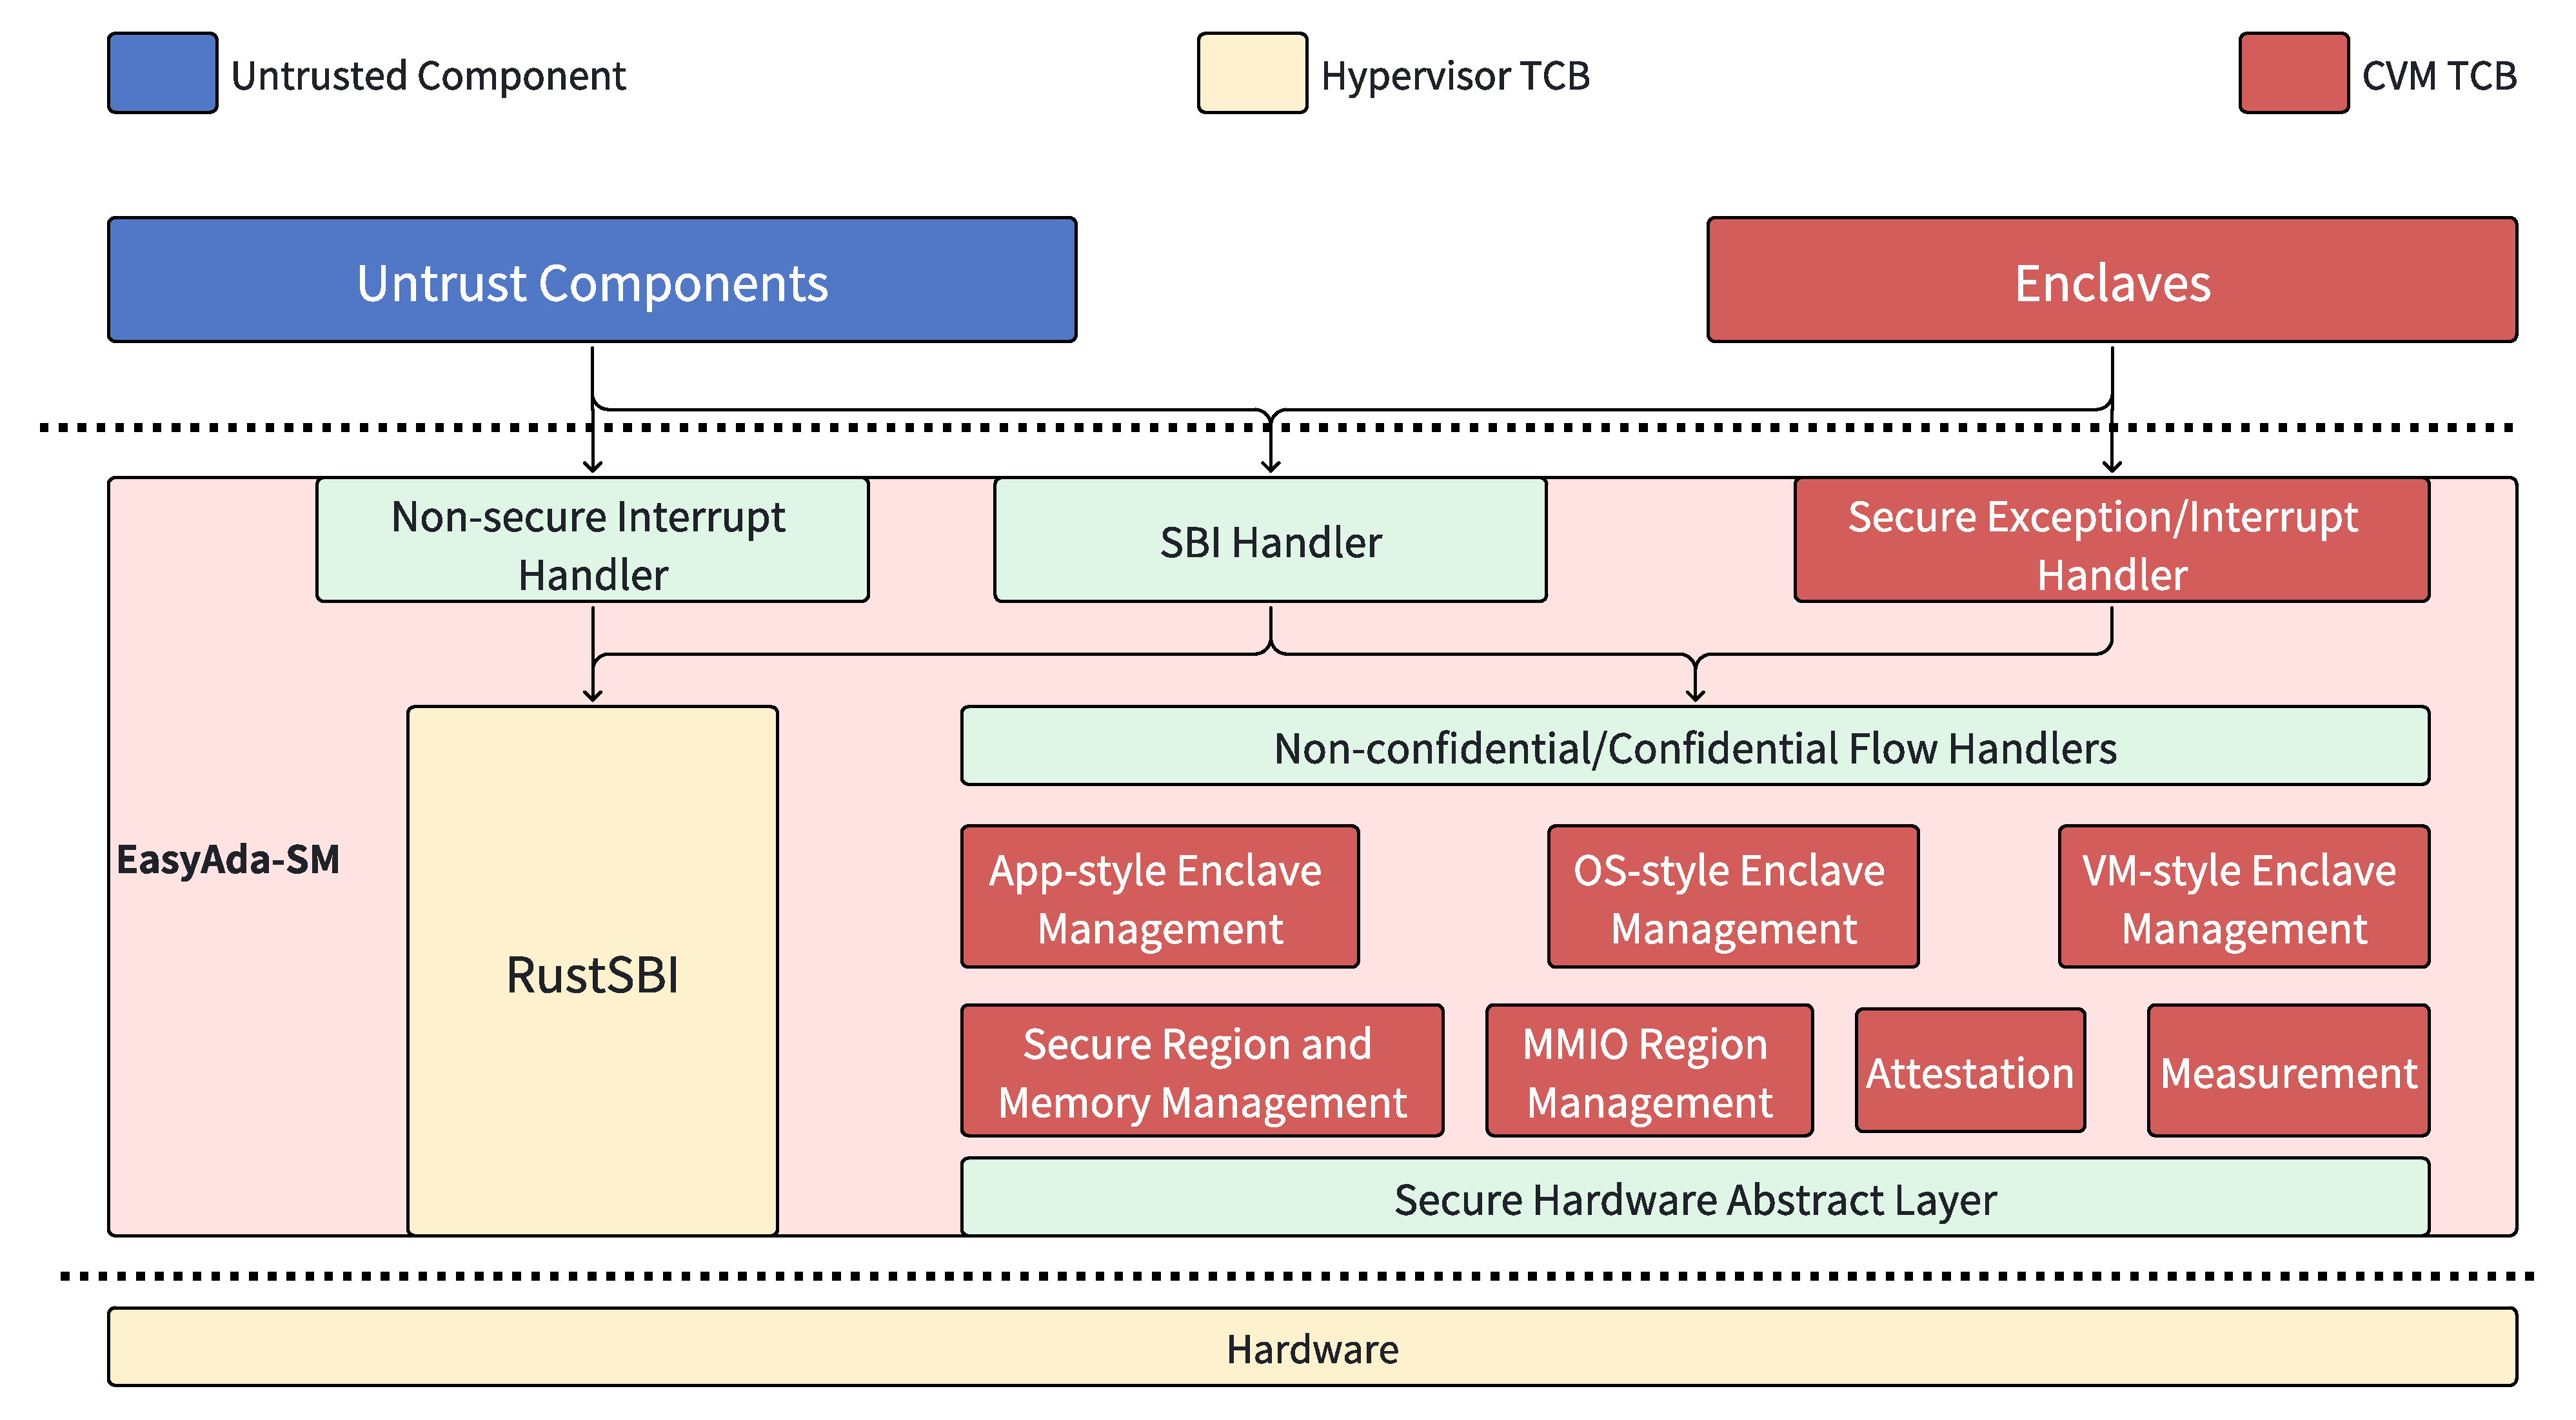
\includegraphics[width=1\linewidth]{sm_arch.pdf}
		\caption{EasyAda-SM总体架构}
		\label{sm_arch}
	\end{figure}
	
	考虑RISC精简和灵活的特点，RISC-V下所有TEE方案均依赖运行在最高特权级的安全固件（通常称为安全监视器，Secure Monitor，SM）结合指令集拓展对外提供TEE相关原语。但是现有SM存在以下问题：（1）不安全的内存管理：现有SM主要基于非内存安全语言C/C++实现，容易在代码中引入不安全的内存访问，影响TEE整体的安全性；（2）拓展性不足：面向不同场景的TEE间SM设计和实现差别较大，无法为不同场景提供统一的安全底座。

	为了解决以上两个问题，如图\ref{sm_arch}所示，EasyAda-SM重新设计了运行在最高特权级的SM，与Penglai和Keystone将Enclave管理模块作为SBI拓展引入SBI固件不同，EasyAda-SM采用了相反的逻辑，将SBI固件作为SM的静态链接库并引入SBI能力抽象层，SM可以调用SBI固件中的函数获取其提供的能力，并且可以通过切换使用的SBI固件具体实现（如不同硬件供应商提供的SBI固件实现等）充分利用不同SBI固件的差异化能力。

	EasyAda-SM将TEE所需的操作，如内存隔离，密钥管理，镜像度量和安全异常处理等抽象为独立的子模块，每个子模块对外提供统一的操作原语以屏蔽底层硬件和指令集差异。如图\ref{sm_arch}所示，EasyAda-trust开发者可以针对不同的TEE方案开发独立的Enclave管理模块，也可以对特定模块进行修改以适配专有指令和硬件。根据最小特权原则（Principle of Least Privilege，PoLP），每个模块仅被授予完成其特定功能所必需的最小权限集合，从而限制潜在安全漏洞的影响范围。
	

	同时，通过对现有RISC-V主流TEE方案进行深入分析，本文发现不同TEE方案对安全内存管理，使用和隔离机制存在较大差异，在安全启动和中断，I/O隔离等方面的机制和策略则较为共通，如Penglai的SM被设计为实现更灵活和细粒度的安全内存管理，因此需要SM实现安全内存分配能力；Keystone的SM则被设计为一次性内存分配，SM不进行动态安全内存分配，仅负责进行保护；ACE中TSM为了适应CVM二阶段页表的构建，实现了专用的页分配器，充分利用Rust的所有权机制消除了重复分配的隐患。进一步的，EasyAda-SM将内存划分为以下几类并据此设计内存隔离方案。
	\begin{enumerate}
		\item 通用区域和通用内存：任何未被SM标记和保护的片上/外内存都属于通用区域下的通用内存。为了提高系统整体的内存利用率，默认情况下所有内存都是由不可信的host负责管理的通用内存。
		\item 安全区域：被SM标记和保护的连续内存区域被称为安全区域。安全区域由通用区域划分而来，SM会为每个安全区域分配唯一的硬件单元用于实现内存隔离。
		\begin{enumerate}
			\item 安全内存：被SM标记和保护，但是尚未被Enclave使用的安全内存，由SM负责分配和管理。
			\item Enclave内存：被SM标记和保护并且被Enclave使用的安全内存。Enclave内存由SM负责配置和保护，但是在Enclave释放之前SM无权进行释放或再分配。
		\end{enumerate}
	\end{enumerate}
	
	图\ref{secmem_divided}展示了EasyAda-SM的内存管理模式。EasyAda-SM将通用内存视为初始状态（未初始化），Enclave内存视为最终状态（被使用），安全内存作为两者转化的桥梁，处于中间状态（初始化但未使用）。EasyAda-SM引入安全内存作为Enclave内存和通用内存转化的中间层，目的是平衡缩小SM攻击面和提高系统整体内存利用率的两种需求。

	\begin{figure}[!h]
		\centering		
		\includegraphics[width=1\linewidth]{secmem_divided.pdf}
		\caption{EasyAda-SM的内存管理模式}
		\label{secmem_divided}
	\end{figure}

	Keystone没有安全内存的中间状态，通用内存直接转化为Enclave内存，优势是内存管理简单，攻击面较小，劣势是难以在Enclave运行期间动态伸缩内存；ACE则在系统启动时静态划分安全内存和通用内存区域，SM负责从安全内存中为可信VM分配Enclave内存，优势是可以在可信VM运行期间动态伸缩内存，劣势是安全区域在系统初始化时静态划分，容易降低系统整体内存利用率；而RISC-V的CoVE扩展则要求host以物理页为单位捐赠内存并由SM直接转化为Enclave内存，优势是提高了系统整体内存利用率，劣势是SM需要实现多个SBI接口并且完全依赖host侧实现内存管理，显著增加了SM的攻击面。
	
	EasyAda-SM允许SM从host侧动态获取内存并转化为相互隔离的安全区域或归还安全区域到通用内存，然后由SM负责从安全内存中动态分配Enclave启动和运行时需要的Enclave内存。在提高系统内存利用率的同时减少对host侧内存管理的依赖，缩小SM的攻击面，实现两种需求的平衡。
	
	进一步的，EasyAda-SM引入了统一的安全区域和内存管理层（以下简称安全区域管理层）将安全内存相关操作，如创建/销毁安全区域，申请/释放安全内存，隔离安全内存等封装为统一安全内存管理原语。同时，安全区域管理层将安全内存管理原语依赖的硬件操作划分为内存管理和内存保护两个部分，并且抽象出了统一的内存管理原语和内存保护原语，开发者可以根据硬件环境和业务需求提供具体的原语实现。通过提供统一的内存安全原语，安全区域和内存管理层简化了开发Enclave模块的难度；通过抽象统一的内存管理和保护原语，安全区域管理层实现了不同Enclave管理模式间基础代码的复用和可扩展性，开发者对上层透明地复用已有原语或根据场景需求和硬件环境实现新的原语。
	
	\subsection{安全特性设计}
	接下来将介绍EasyAda-trust针对CVM需求设计安全的虚拟化方案。
	
	\subsubsection{安全启动流程设计}
	安全启动的目标是构建可信链（Trust Chain），确保只有由授权用户开发的，未经篡改的可信组件可以加载到TEE中运行，并且最终的安全应用仅能在经过验证的平台上运行并获取敏感I/O数据。
	
	安全启动依赖两对密钥对：（1）硬件供应商提供的签名密钥对；（2）每个设备独有的设备密钥对。签名密钥对作为硬件厂商信任背书，签名私钥由硬件供应商离线保管，用于生成SM的数字签名，而签名公钥则存储在每个可信设备的信任根（Root of Trust，RoT）中，用于在系统启动时验证SM的数字签名。设备密钥对则作为每个设备的唯一标识，设备公钥对用户和开发者开放，用于加密用户验证信息或秘密，而设备私钥存储在设备RoT中，用于解密用户加密信息。
	
	RoT是可信链建立的起点。根据EasyAda-trust的威胁模型，EasyAda-trust将硬件供应商提供的可信硬件（如TPM）和固件（存储在eFUSE和ROM等中的代码和数据）视为RoT。硬件供应商在开发，配置和编译SM时，需要生成SM的数字签名。在RoT启动安全启动流程后，需要生成SM的当前度量值并与数字签名进行匹配，由SM进行下一阶段的安全启动流程。
	
	平台供应商可以根据业务场景使用特定的SM配置，因为Hypervisor和不可信VM不在EasyAda-trust的TCB中，因此默认SM配置下不对Hypervisor进行验证，平台和硬件供应商可以根据需求自行拓展支持对Hypervisor和不可信VM进行验证。
	
	Hypervisor需要在系统运行时动态部署CVM。因为恶意软件攻击者可能尝试拉起恶意的CVM，同样恶意的硬件环境和SM可能绕过CVM验证进行强制部署，因此CVM部署时必须完成CVM与硬件环境的双向验证。为了避免恶意硬件环境强制部署和访问CVM中的敏感信息，EasyAda-trust要求CVM开发者自行提供并使用密钥对敏感代码和数据进行加密，确保只在可信的硬件环境进行解密和部署。
	
	针对验证方式，云服务厂商通常采取远程证明（Remote Attestation），通过远程的可信设备验证当前硬件环境和代码是否可信且未经篡改，只有经过验证的环境和CVM才能成功部署。部分嵌入式环境可能长期部署在网络访问受限的环境中，因此EasyAda-trust默认使用本地证明\citess{localattest}（Local Attest）实现CVM与硬件环境的双向验证。
	
	\subsubsection{安全CPU虚拟化设计}
	EasyAda-Hypervisor能够确保VM间vhart的隔离，VM间不会泄漏上下文信息，但是无法实现EasyAda-Hypervisor与VM间的上下文隔离，因此EasyAda-trust对hart引入了机密流和非机密流以实现不同执行环境间上下文的隔离。
	
	RISC-V的硬件虚拟化扩展引入了虚拟化专用特权级以实现VM间以及VM和host间CPU上下文的隔离。对于不可信VM，SM会将大多数系统级异常委派到Hypervisor进行处理以监控VM的任何敏感行为。但是对于CVM，将异常委派到Hypervisor进行处理会导致VM运行上下文泄露给Hypervisor，因此需要TSM拦截和监控CVM的敏感行为。
	
	与普通VM一样，CVM的hart分配和vhart与hart的关联由Hypervisor完成。为了避免不可信组件访问和篡改CVM上下文，在切换到CVM上下文后会配置其原本由Hypervisor处理的异常直接陷入M态中，通过轻量上下文切换到TSM进行处理。若异常需要由Hypervisor处理，则由TSM进行完整的安全上下文切换，清理所有上下文并切换到Hypervisor上下文进行处理。
	
	\subsubsection{安全内存虚拟化设计}
	内存虚拟化主要涉及为VM分配运行内存，并建立和维护VM运行内存和虚拟设备地址的第二阶段地址映射表。前者用于容纳VM运行时的代码和数据，后者用于实现设备直通和VM间通信等。
	
	不可信组件与CVM间内存隔离：为了实现CVM与不可信组件间的内存隔离，CVM无法直接使用Hypervisor分配的不可信内存作为运行时内存，因此EasyAda-trust引入了安全内存和安全区域的概念。安全内存指由SM配置，使用硬件实现强制内存隔离，不可信组件无法直接访问的内存区域，任何用于存储CVM敏感数据和代码的内存必须使用安全内存以确保其机密性和完整性。EasyAda-trust以安全区域为单位管理安全内存，每个安全区域标记了一片物理连续的内存区域，由绑定的硬件和SM进行保护，安全区域内的内存分配由SM负责。安全内存由不可信内存转化而来，Hypervisor可以申请一块连续的不可信内存捐献给SM，由SM进行保护，并将其标记为安全内存，之后任何不可信组件都无法直接访问这片内存区域。
	
	CVM间内存隔离：虽然CVM被视为EasyAda-trust软件TCB的一部分，但是CVM中的代码漏洞可能破坏TEE提供的安全保护，并且控制了Hypervisor的恶意攻击者可能运行恶意的CVM以尝试攻击受害CVM，因此CVM间同样需要实现内存隔离。ACE\citess{ace}中所有CVM共享一个安全区域，通过硬件虚拟化提供的二阶段地址翻译实现CVM间内存隔离。虽然这提供了足够的安全防护，但是难以根据需求对安全内存进行动态收缩和扩容。EasyAda-trust支持增加或回收安全区域，多个CVM可以共享一个安全区域以提高内存利用率。CVM间的内存隔离则通过二级段地址翻译实现隔离。
	
	\begin{figure}[!h]
		\centering
		\includegraphics[width=0.75\linewidth]{cvm_mminit.pdf}
		\caption{CVM二阶段页表初始化}
		\label{cvm_mminit}
	\end{figure}
	
	CVM内存虚拟化：CVM在创建VM实例阶段与不可信VM类似，由Hypervisor完成内存申请和二阶段页表初始化等。当用户需要将VM转换为CVM时，Hypervisor驱动通过TSM对外提供的promote接口，将二阶段页表和FDT的IPA作为参数交给TSM。如图\ref{cvm_mminit}TSM首先会遍历由Hypervisor为当前VM维护的二阶段页表，申请安全内存用于构建完全一致的页表作为CVM的初始二阶段页表，同时按序申请安全内存用以拷贝不可信内存中的数据，避免后续Hypervisor篡改初始状态。
	
	然后TSM将按序遍历CVM的二阶段页表并度量FDT，kernel和initrd的初始度量值（具体CVM度量流程设计将在后续安全启动小节详细说明），并与CVM开发者提供的初始度量值进行对比，若度量值校验通过则说明当前VM符合预期，由可信的开发者开发并且没有被Hypervisor篡改，允许被拉起并访问开发者提供的用于后续加解密I/O数据的密钥。
	
	安全MMIO区域隔离：RISC-V采用统一编址模式，设备的MMIO区域以内存区域的方式进行管理。因此EasyAda-trust基于安全区域与不可信组件的隔离实现了设备MMIO区域与不可信组件的隔离，并且通过为安全区域引入额外的标识符，标识当前安全区域类型是否为MMIO区域，并且可以进行进一步细分实现具体设备类型的标识。
	
	不可信共享内存：除了存储数据和代码的安全内存，CVM与不可信组件间需要额外的共享内存以实现高效的数据交换，尤其针对磁盘等块设备的I/O虚拟化场景。EasyAda-trust支持CVM向不可信host请求共享内存。
	
	不可信共享内存由host分配和管理，主要用于VM间，VM与host间，以及不可信组件与CVM间的数据交换。host完成内存分配后，需要由Hypervisor映射到VM地址空间内，或由TSM映射到CVM地址空间内，确保组件可以在当前地址空间下直接访问共享内存。因为不可信共享内存由host管理，因此CVM在读写这类内存时，需要进行严格的安全检查并主动对敏感信息进行加密避免泄露。
	
	EasyAda-trust并不支持在CVM间分配可信共享内存。因为（1）根据角色划分，VM和CVM均由同一角色——EasyAda-trust用户负责开发，应用功能在开发时已经相对确定，不需要也不应该将需要大量数据交换的多个功能拆分到多个CVM中实现（2）CVM和TSM作为TCB应当尽可能保证精简，在CVM间支持可信共享内存会进一步增加TCB的大小和复杂度（3）少量的数据交换可以通过不可信共享内存和加密信道实现CVM间的数据交换。综上，EasyAda-trust的设计并未考虑使用可信共享内存实现CVM间通信。
	
	\subsubsection{安全中断虚拟化设计}
	中断安全分为两个部分：中断发送的安全和中断接收的安全。两者都要求目标的中断不应被不可信组件获取和篡改。
	
	对于发送中断，RISC-V要求所有中断必须在M态下发送。对于不可信VM，发送中断首先会陷入到Hypervisor驱动中，由Hypervisor驱动决定实际的接收hart，再通过SBI调用陷入SBI固件进行中断发送。在这个流程中Hypervisor对VM的中断有绝对的控制权。但是在CVM场景下，不可信组件无权控制CVM发送的中断，需要直接陷入到TSM中发送，并且需要TSM为CVM维护接收方到物理hart的映射关系。
	
	对于接收中断，SM会将除外部中断外的所有中断全部委派到HS态由Hypervisor进行处理，因为EasyAda-Hypervisor采用静态分区策略，Hypervisor可以进一步将时钟中断直接委派到VS态由VM直接处理，避免频繁陷入Hypervisor带来的性能开销。其他中断如软件中断等需要陷入到Hypervisor中进行处理，由Hypervisor决定是否需要注入中断或切换到vhart服务线程上下文运行，无需对CPU当前上下文进行清理，相关中断配置由Hypervisor负责。
	
	但是对于CVM，除时钟中断外的其他中断必须绕过Hypervisor直接陷入到TSM中进行处理并决定是否需要中断注入。如果中断涉及进一步的上下文切换，需要由TSM负责清理CVM上下文避免泄露任何敏感数据。中断相关配置均由TSM负责。
	
	除了中断发送/接收安全外，还需要额外注意拒绝服务攻击（Deny of Service，DoS），包括CVM对host侧的DoS攻击，以及host对CVM侧的DoS攻击。前者由于host具有最高调度权，可通过TSM强制销毁恶意CVM来解决；而针对后者（host攻击CVM），则需要进一步区分攻击模式：一种攻击模式是host生成大量伪造的中断请求，迫使CVM频繁陷入TSM，导致CVM无法及时响应其他正常请求，这种攻击可以通过TSM对来自host侧的中断进行监控和计数，进而对中断请求进行管控和屏蔽实现防御；另一种攻击模式则是host拒绝响应来自CVM的任何请求，因为host被设计为负责管理系统资源，所以不针对这种攻击进行防御。
	
	\subsubsection{安全I/O虚拟化设计}
	EasyAda-Hypervisor原有的安全I/O虚拟化方案能够实现：（1）VM间数据流和控制流的隔离（2）确保同一时刻一个设备仅能划分给一个软件实体（VM或Hypervisor）直接访问。
	
	为了确保CVM使用的外部设备的安全性，EasyAda-trust需要额外实现以下安全能力：
	\begin{enumerate}
		\item 平台和硬件的可信性验证：根据当前设备的安全级别，在CVM使用安全设备之前对设备进行可信验证，防止CVM被恶意外设攻击导致敏感数据的泄漏和篡改。
		\item CVM生命周期中I/O数据的安全性
		\begin{enumerate}
			\item CPU侧数据安全性：保护CVM访问外设过程中输入输出数据的机密性和完整性，包括通过设备独占，数据加密和校验等方案实现。
			\item 设备侧数据安全性：具备DMA能力的设备可以绕过CPU侧的内存隔离机制直接访问物理内存，恶意设备可以利用这一点直接读写安全区域，因此需要根据外设安全级别限制外设可访问的内存区域。
		\end{enumerate}
	\end{enumerate}

	针对以上安全需求，EasyAda-trust根据外设的使用特点将设备划分为两类：
	\begin{enumerate}
		\item 普通I/O设备：这类I/O设备包括串口，网卡，磁盘等设备，这些设备的特点是设备对数据内容不敏感，无需或仅需少量计算。
		\item 安全设备：这类设备重视安全性，对输入数据内容敏感或需要进行大量计算，如指纹采集器，摄像头和硬件加速器等。
	\end{enumerate}
	
	EasyAda-trust根据设备类型采取了不同的可信性验证方案。对于由host管理的普通I/O设备，EasyAda-trust不对其进行可信验证。而对于安全设备，EasyAda-trust采用了host分配，TSM鉴权和管理的逻辑，并在安全启动流程中引入了可信设备注册，使用和回收的可信链。以系统开发时硬件供应商提供的可信硬件配置文件作为可信链起点，。在host未将可信设备提升为安全设备时，仍然可以正常控制该设备，同时host可以在系统运行过程中向TSM请求提升设备为安全设备，由TSM根据硬件配置文件对设备进行可信验证，只有通过验证的外设会被视为可信设备并提升为安全设备。因为CVM在启动时会对硬件环境进行验证，未通过验证的硬件环境无法对CVM核心的机密代码和数据进行加解密，因此由TSM负责对外设进行可信验证是符合可信链建立流程的。
	
	完成设备的可信验证后，EasyAda-trust需要进一步保护机密I/O数据，对于CPU侧的保护，有三种思路可以用于保护CVM的输入输出数据：
	
	1.基于纯加密的数据保护：如图\ref{iosec_encrypt}所示，因为系统设备主要用host负责管理，最简单的方案是CVM使用开发者提供的密钥对所有I/O数据进行加解密和度量，并通过不可信的共享内存和VirtIO协议栈实现与不可信组件的数据交换。最终由host侧的vhart服务线程调用实际外设驱动完成对外设的读写。
		
	这种保护模式适用于纯粹的I/O请求保护，如网卡设备，串口，磁盘块设备等。由CVM作为数据发送者对数据进行度量和加密，用于加解密的密钥仅在安全内存中才会以明文形式存储和使用。而数据使用者通过配对的密钥进行解密和度量，阻止信道上任何潜在的攻击者进行窃听，可以有效保障数据的机密性。但是一方面，因为需要由不可信组件读写数据，需要额外的重传机制保障数据的完整性；另一方面，多数计算任务要求数据以明文形式提供，对数据进行加解密会引入额外的性能开销。
		
	2.基于临时设备授权的数据保护：如图\ref{iosec_temp}所示，如果将设备管理和授权剥离，将设备授权提升到SM进行管理，由SM在不可信组件和CVM间实现设备的分时授权，确保同一时刻一个设备仅能授权给一个CVM或不可信组件使用，当一个实体获得授权之后，其他实体无权对设备进行任何读写和配置操作。
		
	这种保护适用于全局唯一设备的I/O请求保护。在软件实体获得授权时可以获得设备的完全访问和配置权限，当CVM获取授权时，可以直接使用明文数据读写设备而不用担心不可信组件和其他CVM劫持设备或窃取和篡改数据；同样的，当不可信组件获取设备授权时，CVM也无法劫持或访问设备；当解除权限时，由SM或软件实体自身清理设备状态，避免泄露敏感信息。这种模式可以在保护数据机密性和完整性的同时，避免加解密带来的开销。但是这种保护方式需要额外引入复杂的时分复用逻辑，尤其对于在内核态下直接进行管理的设备，需要对内核进行修改以确保SM可以正确监控系统对外设的使用，避免因为调整设备授权导致当前实体对外设的访问异常中断。
		
	3.基于硬件分区的数据保护：如图\ref{iosec_part}所示，若当前硬件环境中存在冗余或专为安全应用设计的设备，参考静态分区的思想，可以对设备进行分区，将部分设备固定划分给可信组件使用的同时，避免影响不可信组件对外设的访问。如ARM下安全世界拥有独立的UART，GPIO，flash和RAM等设备专供安全世界使用。
		
	这种保护模式适用于专用安全设备或冗余外设的I/O请求保护，如指纹/声纹输入设备，冗余串口/flash等。因为RISC-V采用统一内存编制，硬件分区可以基于内存隔离机制实现，CVM可以以明文形式直接读写TEE外设，无需额外的加解密工作；同时CVM和host侧因为访问独立的外设，I/O流程完全隔离，对外设的访问互不干扰，在保证数据完整性和机密性的同时具备更高的效率，且无需在host和CVM间实现复杂的时分复用逻辑。但是一方面该方法对硬件环境有较高要求，在硬件资源受限的环境中难以使用；另一方面可扩展性不足，如果存在多个CVM实例，CVM间仍然需要针对设备实现时分复用逻辑。
	\begin{figure}[!htb]
		\centering
		\subfloat[基于密码学的I/O数据保护框架]{
			\includegraphics[width=0.4\linewidth]{iosec_encrypt.pdf}
			\label{iosec_encrypt}
		}
		\hfill
		\subfloat[基于临时设备授权的I/O数据保护框架]{
			\includegraphics[width=0.4\linewidth]{iosec_temp.pdf}
			\label{iosec_temp}
		}
		\hfill
		\subfloat[基于硬件分区的I/O数据保护框架]{
			\includegraphics[width=0.4\linewidth]{iosec_part.pdf}
			\label{iosec_part}
		}
		\caption{CVM的I/O数据保护机制}\label{iosec_frame}
	\end{figure}
	
	对于普通I/O设备，EasyAda-trust允许CVM不保护I/O数据（如串口输出）或参考\ref{iosec_encrypt}方法保护I/O数据，设备直接授权给host使用，CVM和不可信VM需要通过不可信的共享内存与host通信，由host完成对外设的实际操作。简化设备的管理逻辑，同时确保设备可以扩展给更多组件使用。
	
	而对于安全设备，EasyAda-trust参考\ref{iosec_part}方法，由CVM直接独占设备进行管理，SM负责实现设备的数据缓冲区和MMIO区域与不可信组件间的隔离。CVM仍然可以通过共享内存的方式与其他组件间进行交换数据。为了避免复杂的运行时设备发现，EasyAda-trust要求开发者在开发阶段对完成可信设备的标记并将可信的硬件配置存储在硬件RoT中或直接固化在TSM中，用于对设备身份进行验证。
	
	对于设备侧的I/O数据保护，EasyAda-trust基于RISC-V的IOPMP扩展实现。为了避免IOPMP条目的快速耗尽和频繁的IOPMP切换，EasyAda-trust对安全设备仅开发所有由host分配的安全区域的访问权限，而非安全设备仅能访问不可信的内存区域，具体IOPMP管理方案实现将在安全监视器章节详细介绍。
	
	同时，必须考虑到部分端侧硬件环境出于功耗和成本考虑，仅实现了RISC-V硬件虚拟化扩展而未实现IOMMU，并且外部设备本身不具备地址管理单元（Memory Management Unit，MMU）。因此EasyAda-trust在部分硬件环境中无法使用IOMMU实现I/O虚拟地址（Input/Output Virtual Address），使用IPA直接配置DMA会导致外设的内存访问触发未定义的行为，必须要通过软件实现IPA到HPA的地址翻译。一种方案是在此类环境上整体回退到全虚拟化设备，CVM仍然具备完整的设备驱动，但是任何对MMIO设备的访问都需要陷入到TSM中完成地址翻译和硬件操作，对于性能敏感场景会引入无法接受的时延和性能开销。因此EasyAda-trust在保留了全虚拟化支持的基础上，允许CVM显式向TSM发起请求批量实现IPA到HPA的翻译，仅需在配置DMA地址时触发一次下限，并且可以通过合并I/O请求进一步降低地址翻译的开销。
	
	为了实现CVM使用硬件加速器计算时数据的机密性和安全性，下面将详细介绍基于EasyAda-trust的安全异构计算环境的设计。

	\subsubsection{安全异构计算环境设计}
	与其他I/O设备相比，硬件加速器丰富的软硬件计算和存储资源增加了I/O数据保护的难度；同时，因为硬件加速器承担了大量的计算任务，对性能非常敏感；而且与其他设备类似，需要考虑跨执行环境的设备复用。	前文已经介绍了通过数据加密和独占设备的I/O数据保护，但是这些措施在实现CVM数据保护时存在一定的局限性：
	\begin{enumerate}
		\item 纯密码学方案的吞吐开销：对于资源稀缺的嵌入式场景，安全性并非硬件加速器的第一考量，因此通常并不具备硬件加解密能力，需要通过软件方案加解密，如果采用3-7（a）的方法进行保护，对于AI训练中的大规模梯度同步，密码学操作会迅速占满显存控制器的带宽或CPU的计算周期，导致严重的计算延迟并显著降低带宽利用率。Lee\citess{gputee_performance}等人的研究显示这种开销导致DDP训练迭代时间平均增加了8倍，极端情况甚至达到41.6倍。同时，密码学基于块的计算方式与GPU非连续的内存访问间粒度不一致，会进一步放大加解密的负面影响。
		\item 独占设备难以满足复杂场景：复杂嵌入式场景下通常需要部署多个模型以应对不同的使用场景，如车载场景下座舱AI和自动驾驶模型通常位于不同的执行环境中，均需使用硬件加速器进行计算。因此EasyAda-trust被设计为支持在不可信组件和CVM间共享的硬件加速器。
	\end{enumerate}
	
	根据硬件加速器与CPU的耦合程度，可以将其划分为以下三类：（1）指令集扩展，将AI运算逻辑直接嵌入CPU流水线中，集成度最高；（2）协处理器，与CPU共享物理内存并通过MMIO进行控制，集成度次之；（3）片外加速器，拥有独立显存，自由度最高，通常在服务器等高性能场景下使用。端侧场景下为了控制功耗和成本，主流硬件平台中硬件加速器通常以协处理器的模式集成在SoC中，以统一内存架构（Unified Memory Architecture，UMA）的方式进行管理。因此除了隔离硬件加速器的MMIO区域外，还需要额外隔离从内存中动态分配的数据缓冲区。
	
	\begin{figure}[!h]
		\centering		\includegraphics[width=0.7\linewidth]{iosec_arch.pdf}
		\caption{硬件加速器管理CVM设计}
		\label{iosec_arch}
	\end{figure}
	
	如图\ref{second_tcb}所示，EasyAda-trust为了降低用户安全管理硬件专用加速器的难度，实现为不同的硬件加速器提供统一的保护方案，引入了专用加速器管理CVM（Accelerator CVM）。得益于CVM的引入，开发者可以实现对现有硬件加速器驱动的复用而无需进行代价高昂的移植。
	
	对于CPU侧，与其它安全设备类似，有TSM通过安全硬件实现硬件加速器MMIO区域与不可信组件的隔离。而对于硬件加速器使用的动态数据缓冲区，因为数据缓冲区由加速器驱动从CVM的安全内存中进行分配，同样可以复用安全区域提供的内存隔离保障。对于外设侧，TSM会通过IOPMP授予且仅授予硬件加速器访问管理CVM的使用的安全区域的访问权限，由TSM确保不会因为错误配置DMA导致硬件加速器I/O地址异常。得益于I/O数据保护，CVM可以直接以明文数据形式与硬件加速器进行交互，避免了高昂的加解密开销。
	
	为了实现硬件加速器在不同执行环境间的复用，加速器管理CVM可以作为半虚拟化设备后端，为其它不可信组件提供虚拟硬件加速器设备。不可信组件和加速器管理CVM间的虚拟设备发现同样在开发时通过配置硬件配置文件静态实现。因为EasyAda-trust的首要目标是确保CVM内机密应用和数据的安全性，对于不可信组件则不进行任何保障，因此不可信组件和加速器管理CVM间使用不可信的共享内存进行数据交换，并且不强制要求任何数据加密和校验。	
	
	\section{本章小结}
	本章系统论述了基于RISC-V架构的微内核虚拟化方案EasyAda-trust的架构设计与核心机制。该方案以EasyAda和EasyAda-Hypervisor微内核虚拟化方案为底层支撑，通过引入Rust编写的安全监视器EasyAda-SM及内存原语抽象，有效缩减了系统的TCB。在安全机制方面，建立了涵盖机密虚拟机全生命周期的防护体系，利用本地证明、机密流隔离及二阶段页表等技术，保障了CPU状态与内存空间的强隔离性，并构建了抗攻击的安全中断处理路径。此外，针对端侧异构计算需求，方案结合IOPMP技术设计了专用加速器管理机制，在提升设备复用效率的同时确保了数据的机密性。

	\chapter{内存安全的模块化安全监视器实现}
	
	\section{内存安全固件}
	为了消除SM中不安全的内存访问，EasyAda-SM使用适合嵌入式场景的内存安全语言Rust实现，通过静态的编译时内存检查消除代码中可能存在的不安全内存访问，避免了昂贵的运行时内存检查和回收。EasyAda-SM基于RustSBI\citess{rustsbi}而非基于内存不安全语言C的SBI固件（如OpenSBI），进一步消除了SBI固件中不安全的内存访问。
	
	\section{安全区域和内存管理层实现}
	\begin{figure}[!h]
		\centering		
		\includegraphics[width=0.8\linewidth]{sec_region.pdf}
		\caption{安全区域和内存管理层实现}
		\label{sec_region}
	\end{figure}
	安全区域和内存管理层的目标是实现不可信组件与安全内存间隔离的同时提高系统整体的内存利用率。如图\ref{sec_region}所示，安全区域和内存管理层以安全内存管理器作为安全内存的顶级管理单元，对外提供安全内存管理接口，每个安全内存管理器包含多个安全区域（Secure Region）和一个安全内存保护器。
	
	每个安全区域关联一块连续内存区域和一个内存分配器（allocator），内存分配器对应一套内存管理算法实现。严格来说安全区域管理的内存在被强制隔离之前并不属于安全内存，因为不同TEE方案对于安全内存的保护时机存在较大差异，因此EasyAda-SM将安全内存保护器和allocator分离，由安全内存管理器自行决定内存的保护时机，为了方便叙述，后文以安全内存代指安全区域管理的内存区域。
	
	安全内存保护器则负责管理用于隔离安全内存的安全硬件如PMP,并对外提供内存保护接口。安全内存保护器的保护粒度是安全区域，主要目标是隔离不可信组件和安全内存，并辅助实现Enclave间内存隔离。
	
	为了在同一Enclave管理模式下提供统一的安全内存视图，每个Enclave管理模块通常使用一个全局的安全内存管理器实现统一的安全内存管理，并使用每个安全区域独立的allocator实现精细化的内存管理。
	
	根据上一章中介绍EasyAda-SM的分层设计思想，安全内存管理器抽象了安全内存管理原语，allocator抽象了内存管理原语，而安全内存保护器则抽象了内存保护原语，三者共同实现对安全内存生命周期的管理。下面将按序说明每个原语的具体实现。
	
	\subsection{内存管理原语}
	\begin{table}[!ht]
		\caption{EasyAda-SM内存管理原语}
		\label{memmgr}
		\begin{tabular}{p{2cm} <{\centering} p{10cm}<{\raggedleft}}
			\toprule
			原语 & 功能 \\
			\midrule
			new & 创建一个空的allocator（此时无安全内存需要管理） \\
			init & 使用指定连续内存区域初始化一个allocator \\
			alloc & 从当前安全内存中申请内存 \\
			free &  释放安全内存到当前安全区域中\\
			available & 获取当前安全内存剩余可分配内存 \\
			total & 获取当前安全内存总大小 \\
			\bottomrule
		\end{tabular}
	\end{table}
	如表\ref{memmgr}所示，内存管理原语抽象了安全内存管理所需的操作。包括初始化安全内存，申请/释放安全内存等。为了简化实现并避免重复安全检查引入的系统性能开销，内存管理原语不进行任何安全检查，如不在free原语中检查释放内存是否属于当前安全区域以避免破坏内存管理元数据等。
	
	本文分析了不同Enclave抽象的安全内存使用特点：
	\begin{enumerate}
		\item 基于应用的Enclave抽象（App Enclave）：此类轻量化Enclave通常直接运行在用户态，无权访问和控制任何内核态资源，如MMU和中断配置等。因此TA的虚拟地址空间和物理地址空间在Enclave运行时不会进行任何修改。
		\item 基于OS的Enclave抽象（Rt Enclave）：此类Enclave更加复杂，拥有完整的用户态和内核态资源，TA的虚拟地址空间在运行时可能修改；但是因为直接运行在与host相同的特权级，为了保证高效的内存隔离，Enclave的物理地址空间在运行时不会进行修改。
		\item 基于VM的Enclave抽象（VM Enclave）：因为开启了硬件虚拟化，此类Enclave兼具前两种Enclave的特点：在虚拟化特权级下拥有完整的用户态和内核态资源，又可以在运行时无感可控地调整Enclave物理地址空间并且不破坏当前内存隔离。
	\end{enumerate}
	
	EasyAda-SM针对不同类型Enclave使用安全内存的特点，提供了三种参考内存管理原语实现，下面将介绍其具体实现。
	
	\subsubsection{基于空分配算法的原语实现}
	该实现为安全区域的内存管理器的空实现，仅用于安全区域初始化，因为部分关键安全区域（如SM自身代码和数据占用内存区域）仅需要进行隔离，不允许进行任何分配，需要使用空分配算法作为分配器占位符。在空分配算法上尝试调用任何初始化或分配操作都会导致异常。
	
	\subsubsection{基于伙伴分配算法的原语实现}
	Buddy分配器基于对RustSBI现有系统堆管理算法的复用，使用buddy算法管理安全内存，支持多个Enclave共享相同的安全区域。该实现针对App Enclave，以2的幂次为粒度分配和管理安全内存，足以满足App Enclave的内存需求，可以较好的兼顾分配效率和内存利用率，同时内存管理元数据直接存储在安全内存中，对SM本身的内存依赖较少。劣势是为了简化管理逻辑需要预留一部分安全内存用于存储内存管理元数据，在大片内存分配场景下容易产生外部碎片。
	
	该算法可以确保内存分配行为的安全，即同一内存块同一时刻能且仅能属于一个Enclave内存区域。但是对内存块间的隔离不提供任何保障，依赖Enclave管理模块配置MMU实现隔离，因此不可用于Rt Enclave的内存管理。
	
	\subsubsection{基于一次性分配器的原语实现}
	一次性分配器将当前安全区域内所有安全内存作为一个内存块进行分配和释放，同一安全区域仅供一个Enclave使用。该实现专门针对Rt Enclave和安全设备的内存管理。因为Rt Enclave在内存管理上具备两个特点：（1）可以在Enclave内部进行内存分配，利用预留的空闲内存区域（2）可以配置MMU，因此不能通过MMU实现Enclave间内存隔离。而一个安全设备的内存区域应当完全由一个实体进行管理，不应进行拆分。一次性分配器仅对Enclave内存需求和类型进行简单判断，如果类型匹配且安全内存满足Enclave需求，则直接完整分配所有安全内存为Enclave内存，并返回内存信息，由Enclave在内部进行二次内存管理；同时复用安全内存保护器提供的安全区域间隔离实现Enclave内存间的隔离（因为此时Enclave独占安全区域）。
	
	该算法可以确保任意类型Enclave间的内存隔离，并且分配逻辑简单，开销较低。但是因为没有对内存进行任何拆分，对于不具备内存管理能力的Enclave容易引入内部碎片降低内存利用率；同时，安全内存保护器可以使用的安全硬件数量较为有限（如RISC-V PMP条目数量多为16，最多不超过64个），该方法会快速耗尽可用的安全硬件，因此不应大量使用。
	
	\subsubsection{基于页分配器的原语实现}
	页分配器（Page Allocator）是专为虚拟机飞地（VM Enclave）设计的内存管理组件。该分配器充分利用RISC-V架构多级页表支持特定映射粒度（如4KB、2MB和1GB）的特性，并深度结合Rust语言的所有权机制。与依赖不安全内存操作的传统管理方案相比，该设计从根源上消除了内存管理元数据遭破坏的安全隐患。
	\begin{figure}[!h]
		\centering		
		\includegraphics[width=1\linewidth]{pageallocator.pdf}
		\caption{PageAllocator结构}
		\label{pageallocator}
	\end{figure}
	如图\ref{pageallocator}所示，页分配器采用类似多级页表与B树结合的层级拓扑来索引与管理物理内存块。其层级划分严格对齐RISC-V硬件支持的物理页尺寸。分配器中的基本管理单元定义为页令牌，每个页令牌封装了对应物理页的基址与跨度范围，并包含一个子令牌数组，用于指向当前物理页进一步拆分后的次级物理页令牌。依据状态与功能，页令牌可划分为以下三类：
	\begin{enumerate}
		\item 索引页令牌：作为路由与索引节点，该令牌不直接参与物理内存分配，仅负责标识其管辖的次级物理页已被分配或使用。索引页令牌内部动态维护当前内存区域经分割后所能支持的最大单次分配粒度（即最大连续物理页尺寸），从而加速分配时的容量校验；同时，它会为其子令牌数组实际分配内存，以持久化存储次级令牌状态。
		\item 空闲页令牌：作为可供直接分配的叶子节点，该令牌标识其映射的物理页处于完全空闲状态。为优化内存开销，空闲页令牌不会为其子令牌数组预分配实际内存空间。
		\item 已分配页令牌：用于标识对应物理页已完成分配且不可用。在工程实现上，已分配页令牌并非实体数据结构，不占用任何元数据内存。依托Rust的所有权转移语义，一旦某空闲页令牌被分配，其所有权即被消耗，原有资源被自动释放。此机制在编译期确保了该令牌无法被重复引用，彻底杜绝了非法的二次分配。
	\end{enumerate}
	
	分配器初始化阶段：系统首先对目标安全内存区域进行合法性校验，强制要求其基址对齐至4KB物理页边界。为避免直接将理论地址上限（如128TB）作为根节点所导致的内存空间浪费与搜索深度膨胀，分配器会依据实际管理区域的容量动态界定根页令牌的物理页尺寸。随后，分配器遍历安全内存以构建页令牌树。为最小化元数据开销，系统通过计算当前基址所能对齐的最大物理页尺寸来实例化空闲页令牌，并递归查找或建立其父级索引页令牌以完成挂载。遍历结束即标志分配器初始化完成。
	
	页令牌生命周期管理：在分配器初始态，系统中仅存在空闲页令牌与索引页令牌。当处理物理页分配请求时，系统执行如下操作流：（1）自根页令牌发起广度优先搜索，定位首个容量达标的空闲页令牌；（2）若该令牌映射的物理页尺寸与请求严格匹配，则直接消耗此空闲页令牌（逻辑上转为已分配页令牌）并返回物理地址；（3）若其尺寸溢出请求大小，则将该空闲页令牌分裂为若干次级空闲页令牌，原节点降维转化并驻留为索引页令牌，随后对新生成的次级空闲页令牌递归执行上述匹配与分裂逻辑。
	
	在处理物理页释放请求时，系统执行逆向回收逻辑：（1）自根页令牌起始，通过计算目标物理页在安全内存中的绝对偏移量，将其映射为各级索引页令牌的子节点索引；（2）寻址至位移与尺寸均匹配的空缺位置后，利用该物理页重构出新的空闲页令牌并重新挂载入树；（3）执行碎片合并检查，若某索引页令牌下的所有次级节点均已恢复为空闲页令牌，则触发层级合并，消耗所有次级节点并将其父级索引页令牌向上聚合提升为单一的宏观空闲页令牌。
	
	\subsection{内存保护原语}
	\begin{table}[!ht]
		\caption{EasyAda-SM内存保护原语}
		\label{mempro}
		\begin{tabular}{p{3cm} <{\centering} p{10cm}<{\centering}}
			\toprule
			原语 & 功能 \\
			\midrule
			alloc & 申请一个安全硬件用于隔离安全区域，返回ID \\
			free & 根据ID释放一个安全硬件 \\
			disable & 根据ID关闭指定安全硬件 \\
			enable & 根据ID使能指定安全硬件 \\
			grant\_access & 在指定CPU/hart集合中使用指定安全硬件授权访问指定内存区域 \\
			retrive\_access & 在指定CPU/hart集合中使用指定安全硬件限制访问指定内存区域 \\
			is\_protectable & 检查指定内存区域是否可以被保护 \\
			\bottomrule
		\end{tabular}
	\end{table}
	如表\ref{mempro}所示，内存保护原语抽象了隔离安全区域所需操作，包括安全硬件管理和限制/授权指定内存区域访问。
	
	因为不同的安全硬件和内存隔离机制间存在较大差异，如PMP机制下每个条目直接保护连续内存区域，而STT下的MPT条目则存储地址空间的权限表，两者的管理模式完全不同。因此安全内存保护器不对安全设备管理进行约束，仅要求每种实现显式告知安全区域和内存管理层安全区域与硬件的关联关系（alloc/free原语），以及根据关联关系实现对指定内存区域的访问权限控制（grant/retrive）。
	
	因为不同执行环境间通常拥有各自独立的hart，因此RISC-V下硬件内存保护机制通常以hart为单位，每个hart拥有独立的硬件且仅负责配置当前hart内存保护视图。为了实现全局统一的内存保护视图，访存控制配置需要同时同步到所有相关hart，以安全区域为例，SM需要同时完成在不可信组件使用的hart集合中限制访问安全内存和在Enclave使用的hart集合中授权访问安全内存，因此grant和access以hart集合为单位进行配置，不同hart间通过核间中断和原子操作确保配置的一致性。同时，具体的hart集合由更上层的Enclave管理模块管理，内存保护原语仅负责同步配置到指定hart集合。
	
	因为EasyAda-trust主要使用RISC-V PMP机制保护安全内存，因此下面主要介绍基于PMP的内存保护原语实现。
	
	\subsubsection{基于PMP的内存保护原语实现}
	\begin{figure}[!h]
		\centering		
		
\includegraphics[width=1\linewidth]{pmpslot.pdf}
		\caption{PMP槽结构}
		\label{pmpslot}
	\end{figure}
	
	PMP slot：RISC-V下每个hart有独立的PMP条目和相关配置，仅控制当前hart内存访问。为了实现所有hart拥有统一的安全内存视图，如图\ref{pmpslot}所示，PMP管理器以PMP slot为单位管理PMP硬件，每个PMP slot是所有hart上索引相同的PMP条目的集合。
	
	PMP管理器：EasyAda-SM定义的PMP管理器使用位图管理PMP slot，为了提高灵活性，位图中包含三个掩码：（1）当前管理器管理的PMP slot索引的掩码，标记当前PMP管理器管理的所有PMP slot的索引，运行时不可变；（2）当前管理器可分配的PMP slot索引的掩码，标记当前PMP管理器总共可分配给安全区域的PMP slot索引，运行时不可变；（3）当前管理器已分配PMP slot索引的掩码，标记当前PMP管理器中已分配PMP slot索引，运行时动态修改。
	
	在初始化时，开发者初始化当前管理器可使用和管理的PMP slot索引掩码（两者的区别在于，可使用的PMP slot可以动态分配，用于隔离安全区域，而被管理的PMP slot同时包括可使用和开发者预留的PMP slot，如最高权限的PMP slot被用于保护SM，虽然该slot可以被配置，但是不能被使用）。在配置时，安全区域可以选择需要配置的hart的集合，并在这些hart上配置关联的PMP slot限制/授权访问安全内存。
	
	授权/限制访问内存：上层模块可以自由决定本次授权/限制操作覆盖的hart范围。当前请求权限控制时，上层模块需要传入需要控制的内存区域，需要操作的hart集合以及被使用的安全硬件ID。PMP管理器会对安全硬件可用性进行基本检查，然后在当前hart上配置对应的安全硬件，如果涉及多个hart，则需要通过RISC-V下软件中断向远端hart发起请求，确保配置的原子性和一致性。
	
	\subsection{安全内存管理原语}
	\begin{table}[!ht]
		\caption{EasyAda-SM安全内存管理原语}
		\label{secmemmgr}
		\begin{tabular}{p{3cm} <{\centering} p{10cm}<{\centering}}
			\toprule
			原语 & 功能 \\
			\midrule
			new &  创建新的安全内存管理器\\
			init &  初始化安全内存管理器\\
			deinit &  重置软硬件状态并销毁安全内存管理器\\
			extend &  创建一个新的安全区域\\
			reclaim &  回收一个空闲安全区域\\
			alloc\_em &  从符合Enclave类型的安全区域中申请Enclave内存\\
			free\_em &  释放Enclave内存到对应安全区域中\\
			grant\_access & 在指定hart集合上授权访问指定内存区域 \\
			retrieve\_access & 在指定hart集合上限制访问指定内存区域 \\
			\bottomrule
		\end{tabular}
	\end{table}
	
	前文介绍了安全区域和内存管理层对内存管理和保护原语的抽象和实现，本节将介绍安全区域和内存管理层对安全内存管理原语的抽象和实现。如表\ref{secmemmgr}所示，安全内存管理原语总体上可以分为安全内存管理器生命周期管理，安全区域生命周期管理，Enclave内存管理和内存保护四类。
	
	安全内存管理器生命周期管理：安全内存管理器作为安全区域和内存管理层的顶级管理单元，负责统筹安全内存资源和安全硬件资源，并使用安全硬件保护安全内存。在init阶段，安全内存管理器预期完成安全硬件的初始化和关键安全区域的初始化（尤其是SM本身的代码和数据），此时安全内存管理器中不存在可以被用于分配Enclave内存的安全区域，后续可以在安全内存管理器中动态扩展/回收安全区域。在deinit阶段，安全内存管理器会验证所有安全区域的空闲状态。为避免中断Enclave的正常执行，系统强制要求Enclave管理模块在发起deinit请求前，主动完成所有Enclave实例的清理。同时，因为内存清理已经在Enclave内存释放时完成，因此无需二次清理以避免敏感信息泄漏。然后安全内存管理器会消耗所有安全区域的所有权并记录安全内存信息归还到不可信host。
	
	安全区域生命周期管理：安全区域的初始化分为三个部分：内存分配，安全内存隔离，以及内存分配器初始化。内存分配通常由不可信的host完成；在扩展安全区域时，安全内存管理器会首先检查当前安全硬件是否支持保护安全区域，以及是否与已有安全区域重叠，确保不会破坏Enclave间内存隔离。然后安全内存管理器会尝试从安全内存保护器中申请一个安全硬件，使用该安全硬件隔离安全内存和不可信组件，此时安全内存仅能被安全内存管理器访问，最后使用安全内存初始化安全区域，设置当期区域为未使用，完成安全区域初始化，但是内存分配器初始化时机由安全内存管理器自行决定，本文将在后文展示延迟初始化的实现；在回收安全区域时，安全内存管理器会检查安全区域是否是未使用状态，Enclave管理模块必须主动销毁使用当前安全区域的Enclave，然后才能安全回收内存。
	
	Enclave内存生命周期管理：安全内存管理器最终的目标是管理Enclave分配，当Enclave管理模块申请Enclave内存时，需要告知安全内存管理器当前Enclave类型以选择合适的安全区域及内存分配器，安全内存管理器会遍历所有安全区域查找符合类型和内存需求的安全区域，然后尝试申请Enclave内存，如果申请成功则返回内存信息和安全区域编号，否则继续重复该操作直到遍历所有安全区域；当释放Enclave内存时，Enclave管理模块需要提供Enclave内存信息，由安全内存管理器负责遍历所有安全区域并查找Enclave内存属于的安全区域，然后通过安全区域的内存分配器释放Enclave内存。
	\begin{figure}[!htb]
		\centering
		\subfloat[不可信上下文中PMP配置]{
			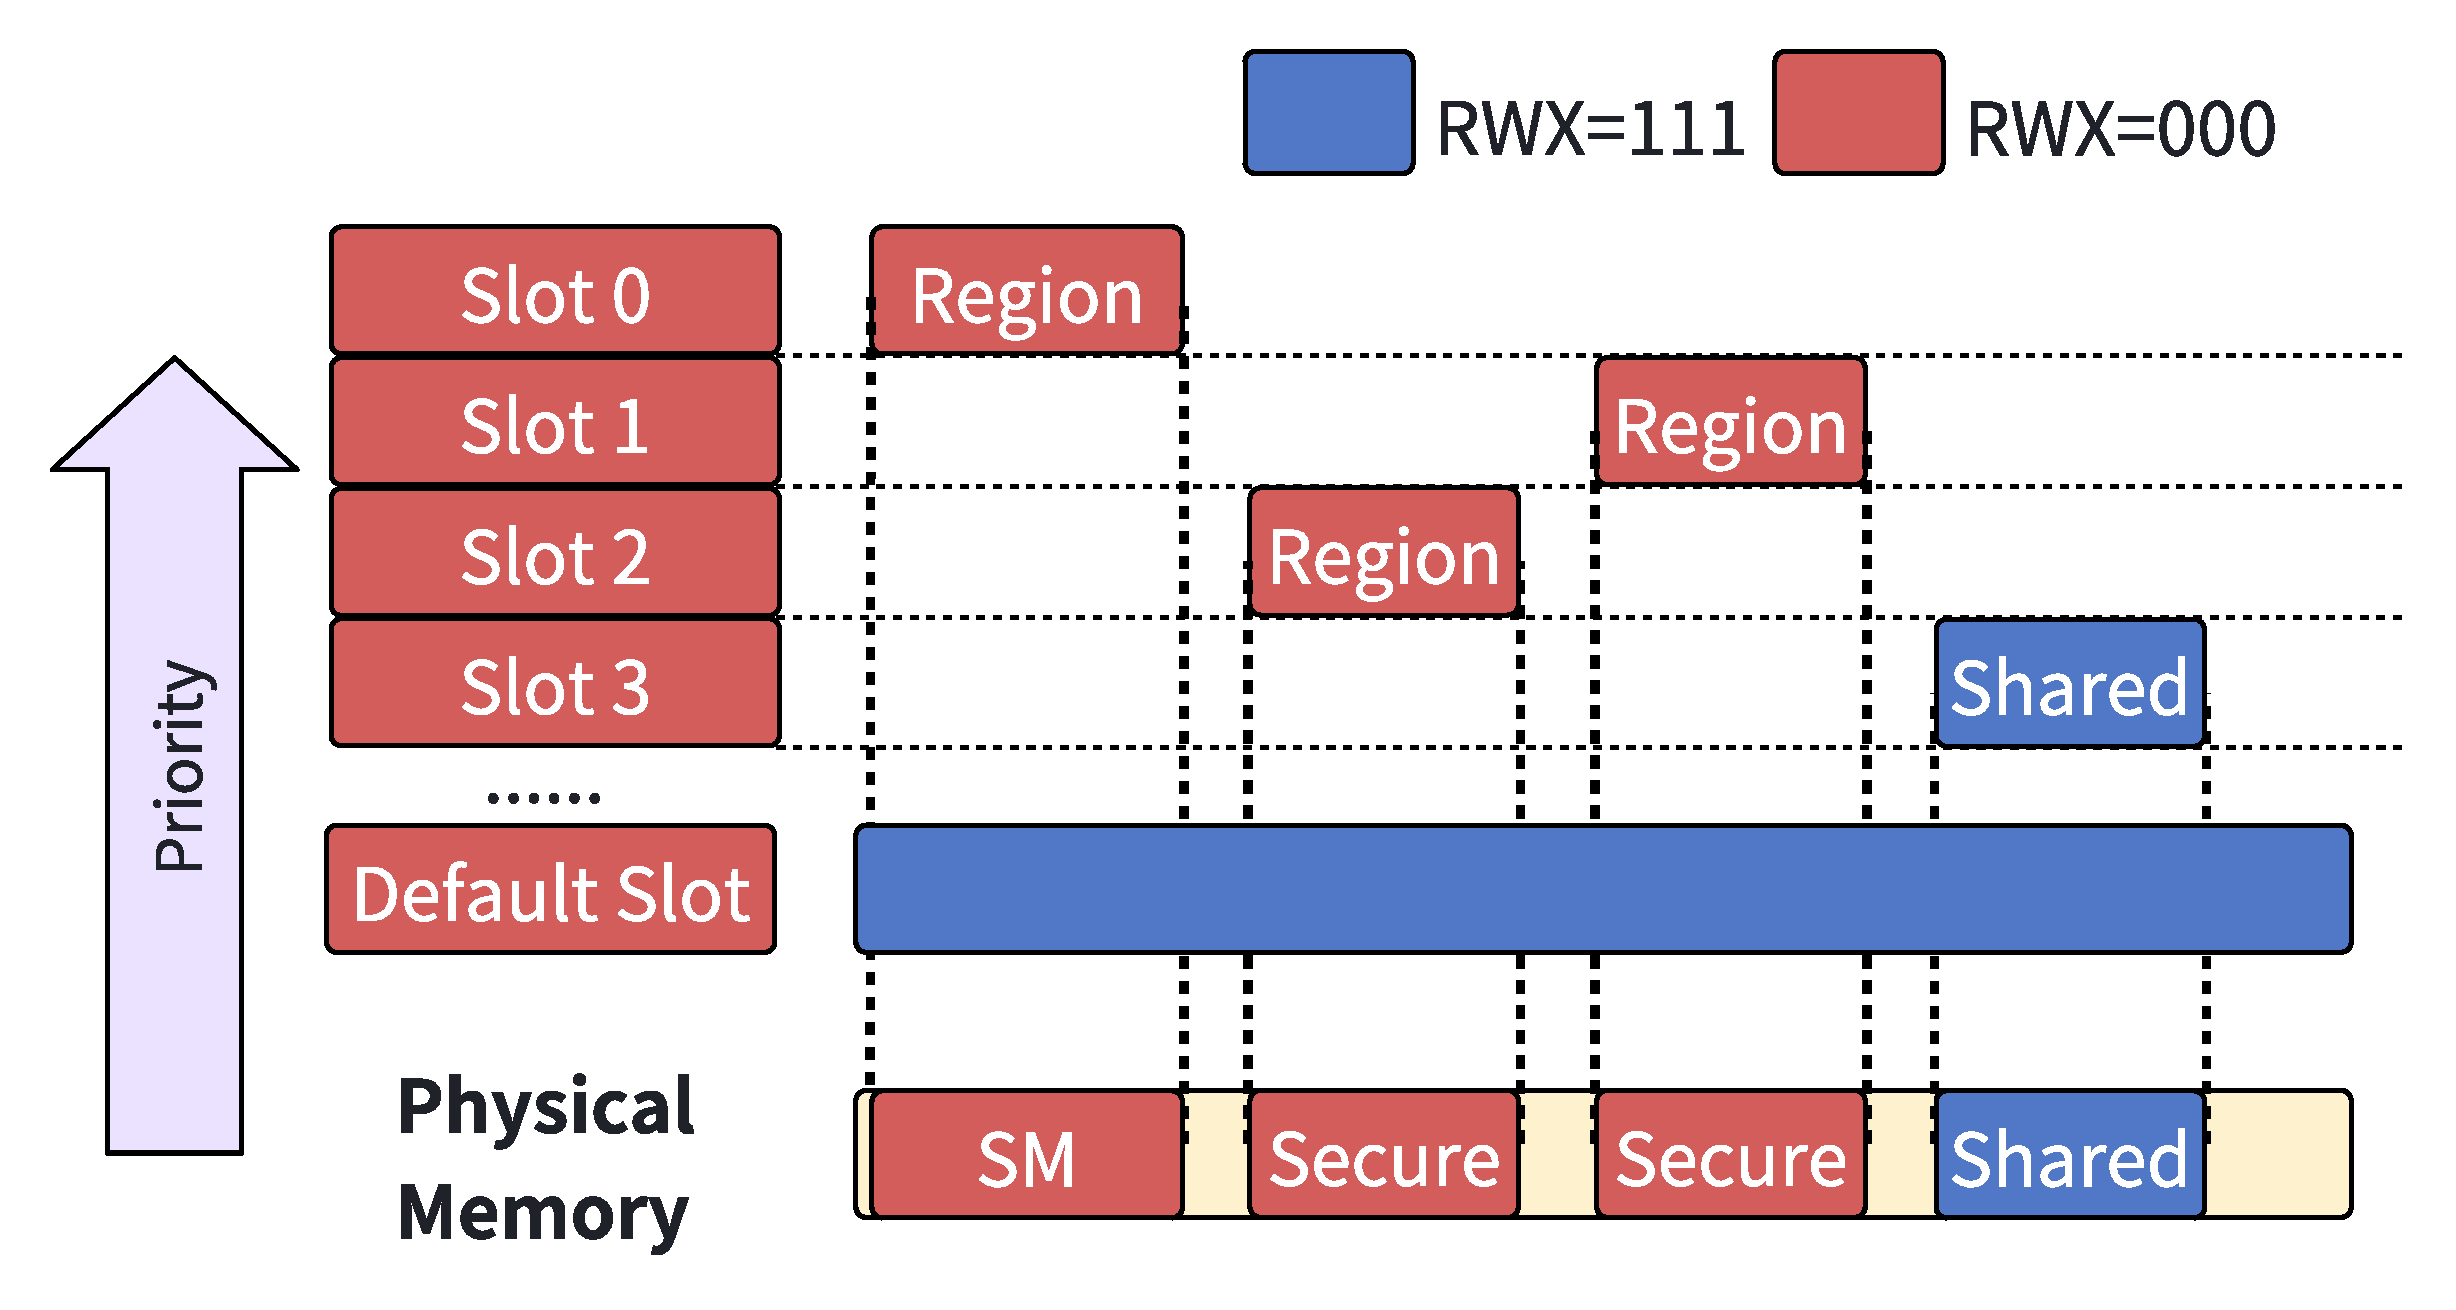
\includegraphics[width=0.4\linewidth]{pmp_iso.pdf}
			\label{pmp_iso}
		}
		\hfill
		\subfloat[可信上下文中PMP配置]{
			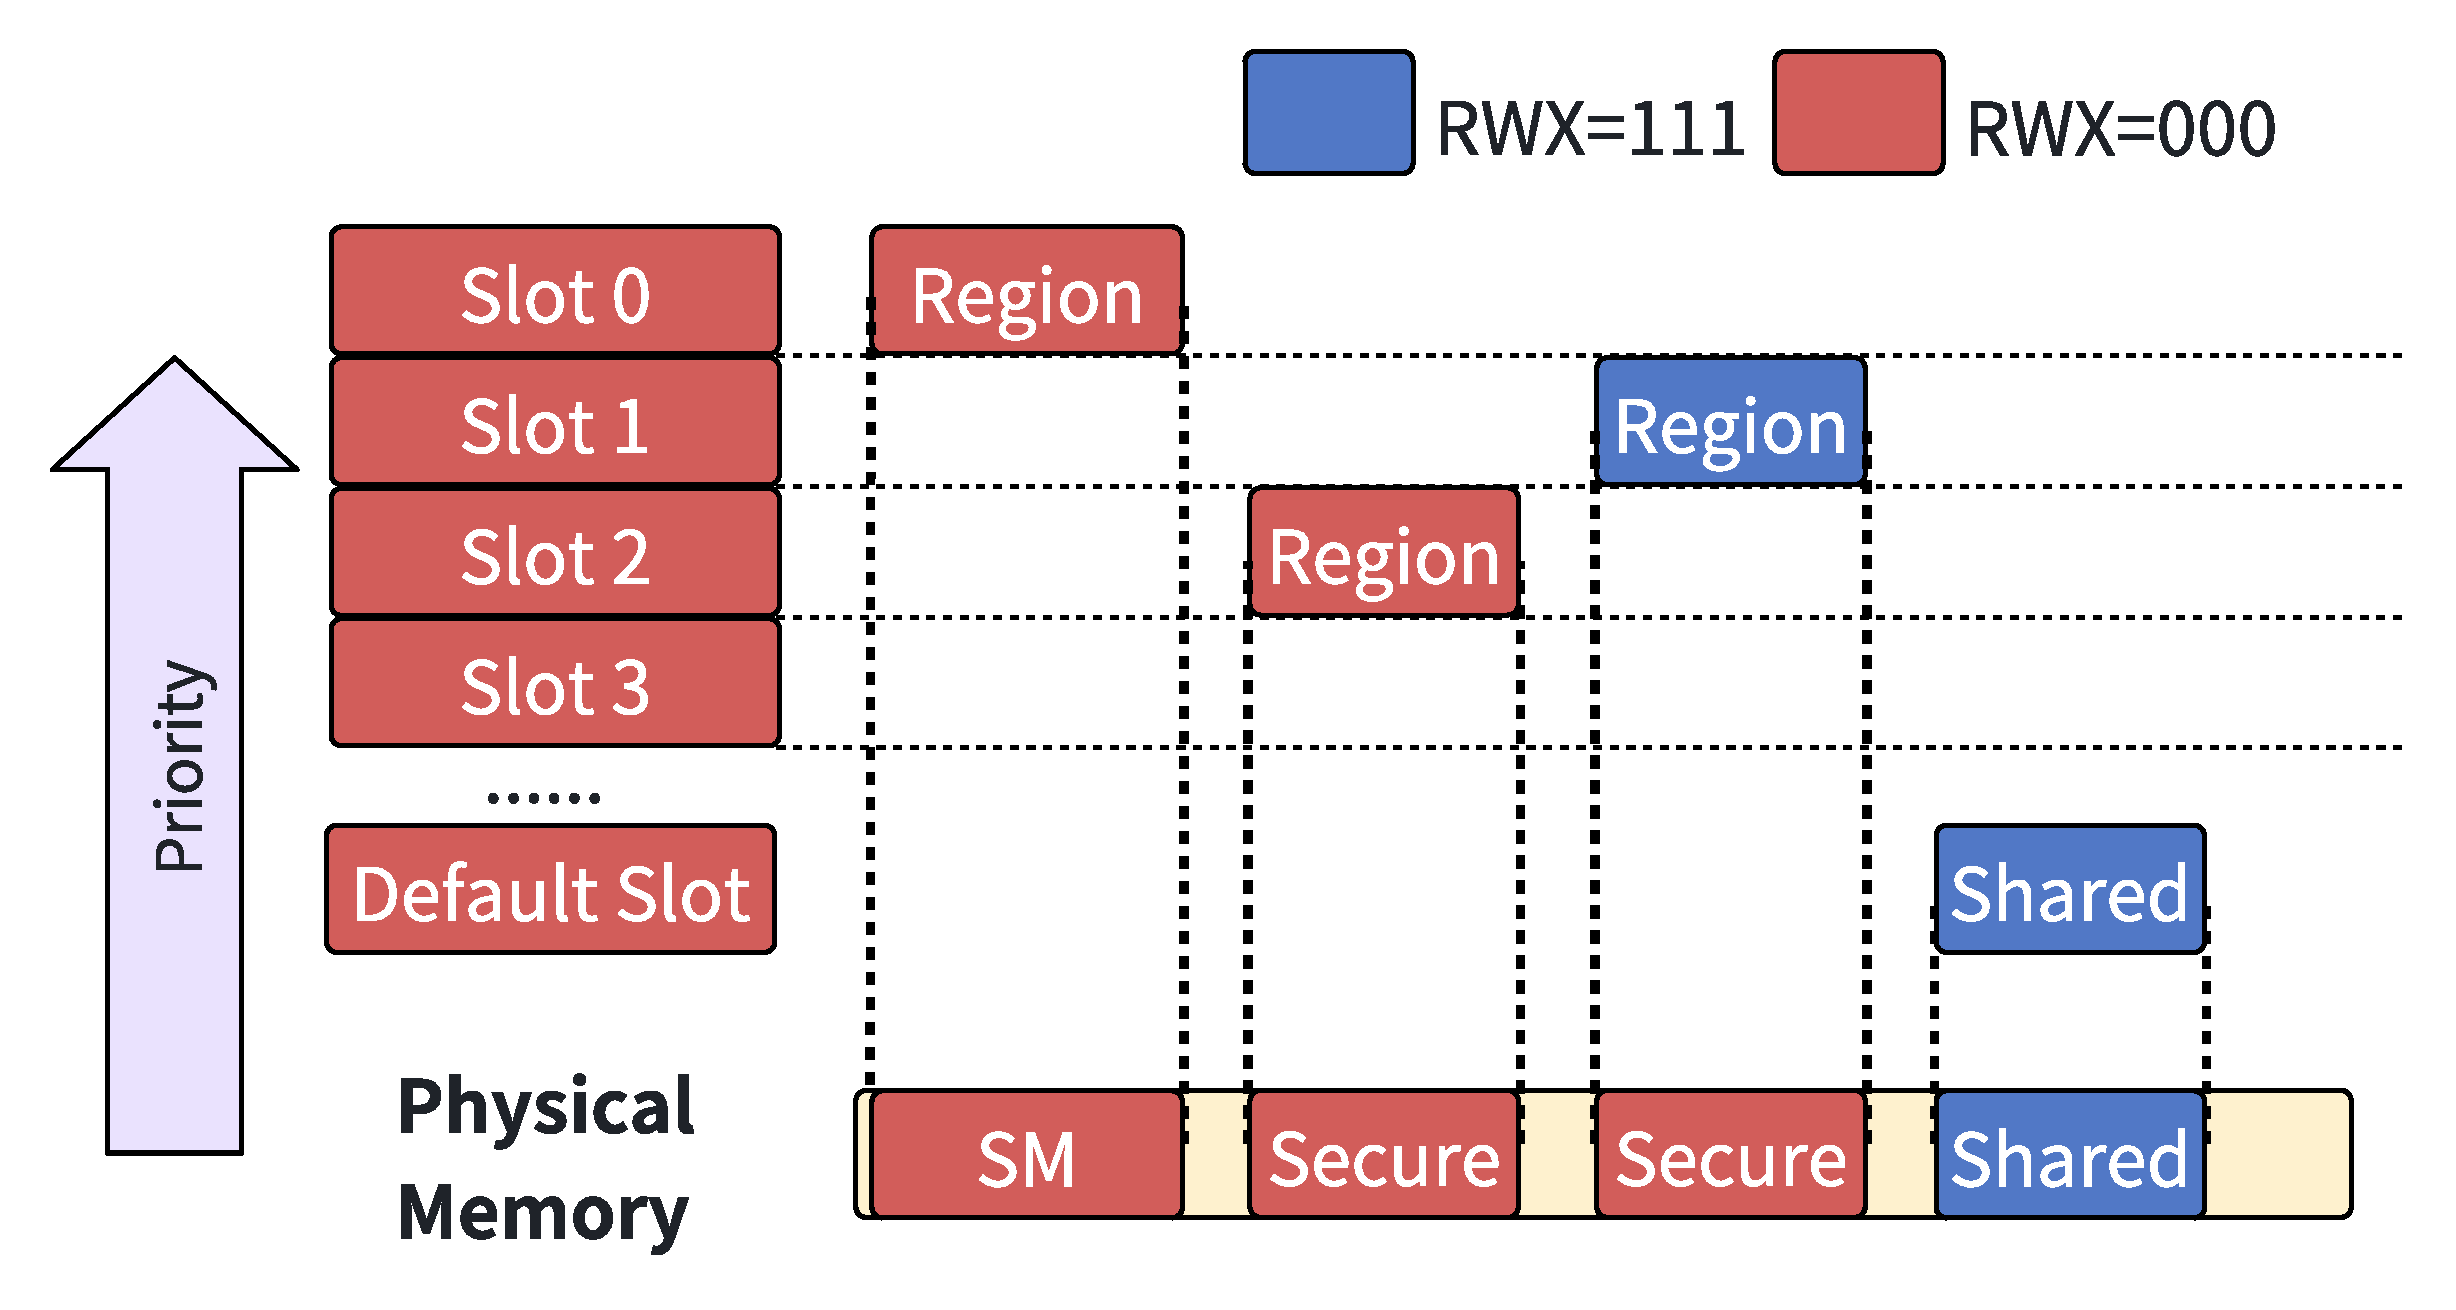
\includegraphics[width=0.4\linewidth]{pmp_auth.pdf}
			\label{pmp_auth}
		}
		\caption{PMP运行时配置}\label{pmp_use}
	\end{figure}
	
	内存保护：如图\ref{pmp_use}所示，本段以PMP为例介绍不安全上下文和Enclave上下文间切换是内存保护配置。对于不可信的上下文，SM会通过retrive限制hart访问任何安全区域，其它内存可以正常访问；而对于可信上下文，SM会通过grant授予hart访问Enclave内存所属的安全区域访问权限。因为复杂Enclave可能使用多个不连续的Enclave内存和多个hart，需要在每个hart上授权访问多个安全区域，并通过hart生命周期管理接口实现其它Enclave使用的hart上下文的安全切换。
	
	这里需要额外关注default slot，该slot用于赋予任何hart默认访问所有内存区域的权限，避免因为保护安全内存导致hart无法访问不可信内存，图\ref{pmp_auth}展示了OS Enclave的管理方式，因为其具备配置MMU的能力且直接运行在内核态下，需要修改default slot禁止访问所有物理内存空间，而对于App和VM Enclave则不强制要求，因为Enclave与MMU相互隔离。
	
	下面将详细介绍EasyAda-SM针对多种Enclave抽象提供统一管理的安全内存管理原语实现。
	
	\subsubsection{面向通用Enclave部署场景的安全内存管理原语实现}
	\begin{figure}[!h]
		\centering		
		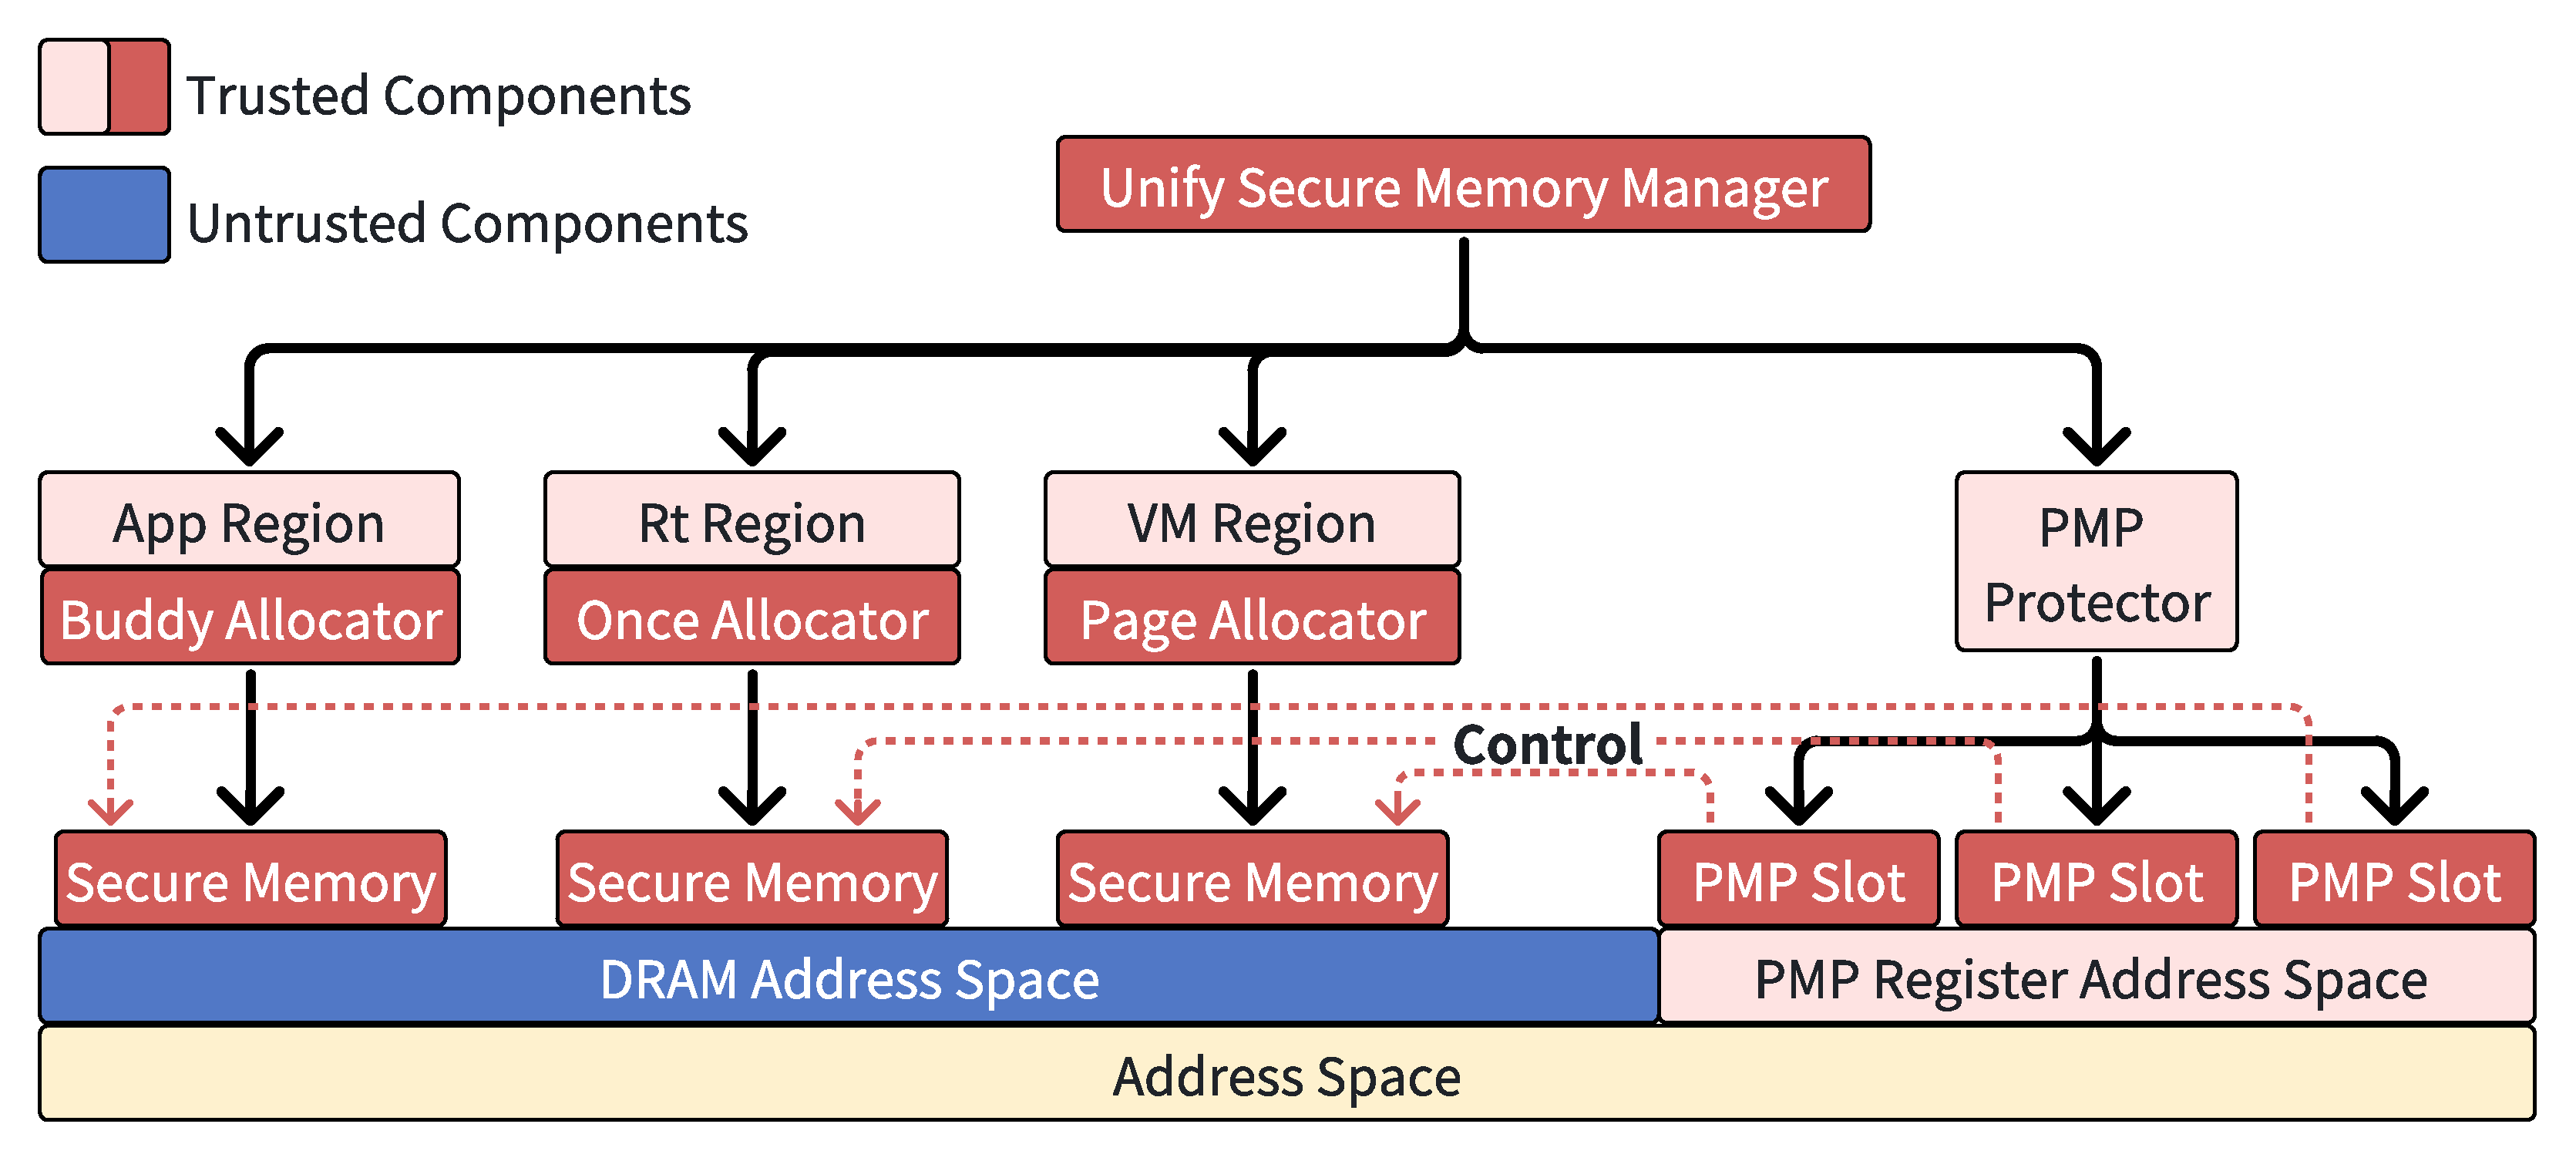
\includegraphics[width=1\linewidth]{unimemmgr.pdf}
		\caption{PageAllocator结构}
		\label{unimemmgr}
	\end{figure}
	为了支持通用的Enclave管理，降低用户开发难度，EasyAda-SM实现了如图\ref{unimemmgr}所示的通用安全内存管理器（简称为通用内存管理器），将Enclave和安全区域划分为一一对应的五类：（1）Application（2）Runtime（3）VirtualMachine（4）Devices（Devices会进一步划分为串口，硬件加速器等设备类型）（5）None（仅用于保护的安全区域），并且如图\ref{Enclave_divided}所示，为每类Enclave绑定了特定的内存分配器。
	\begin{figure}[!h]
		\centering
		\includegraphics[width=0.75\linewidth]{Enclave_divided.pdf}
		\caption{不同类型Enclave与区域类型和分配器的关联关系}
		\label{Enclave_divided}
	\end{figure}
	具体来说，不同Enclave内存与不可信组件的隔离机制相同均基于PMP实现，区别在Enclave内部内存管理和PMP权限配置不同。因此EasyAda-SM引入了通用安全区域表示多种安全区域状态，为了符合Rust的类型检查要求，EasyAda-SM定义了包含所有分配器实现的枚举（类似C/C++中的union），安全区域通过在不同的分配器枚举间切换实现状态切换。并且状态切换按照以下状态机进行。
	
	安全区域状态转换：初始状态下，所有安全区域均为未使用状态，使用空分配器管理内存，仅实现内存隔离，无法进行任何内存分配；当申请Enclave内存时需要显式指定Enclave类型，通用内存管理器会遍历查找类型匹配的安全区域并尝试申请安全内存，若当前类型匹配则直接分配，或者当前区域未被使用则转化为目标Enclave类型区域，初始化内存分配器并尝试分配内存，否则继续查找符合条件的区域；当释放Enclave内存时，通用内存管理器会遍历查找包含Enclave内存的安全区域并尝试释放内存，若释放后安全区域无内存分配，则消耗当前安全区域所有权，转换为未使用安全区域。
	
	除内存管理外，不同Enclave抽象在安全区域保护逻辑上存在较大差异，但是该部分不属于通用内存管理器的职责范围，下一节将介绍如何基于通用内存管理器实现面向CVM的Enclave管理模块。
	
	\section{面向CVM的Enclave管理模块实现}
	\begin{figure}[!h]
		\centering		
		\includegraphics[width=0.6\linewidth]{cvmm.pdf}
		\caption{CVM管理器结构}
		\label{CVM管理模块}
	\end{figure}
	如图\ref{CVM管理模块}所示，CVM管理模块包括四个主要模块：
	\begin{enumerate}
		\item 通用安全内存管理器：如前文所说，通用安全内存管理器目标是实现安全内存与不可信组件间的隔离，负责统一管理安全设备和安全内存区域。
		\item CVM保护器：CVM保护器的目标是实现CVM间的地址空间隔离。因为CVM管理模块使用二阶段地址翻译机制在CVM间实现地址空间隔离的，因此该组件实际负责CVM的二阶段页表管理。
		\item CVM证明器：CVM证明器的目标是实现CVM的可信启动，负责完成CVM初始状态度量，TAP解密和密钥管理。
		\item CVM处理程序：CVM处理程序是CVM管理模块的统一入口，负责实现对不可信组件和CVM所有异常和中断的拦截和处理，机密处理流和非机密流间敏感数据的隔离和安全上下文切换。
	\end{enumerate}
	
	可以将该模块视为TSM的一种实现，后文直接以TSM代指CVM管理器。
	
	\subsection{Enclave间内存安全}
	Enclave间内存安全的核心是隔离不同Enclave的地址空间， 安全内存管理器实现了不可信组件和安全内存间的隔离，如果直接基于其实现CVM间隔离会快速耗尽可用安全硬件，减少可管理的CVM数量。因此TSM利用CVM基于硬件虚拟化扩展运行的特点，引入了CVM保护器基于二阶段页表管理和实现Enclave间内存安全。
	
	CVM保护器的核心职责是维护当前CVM的二阶段页表，包括初始化CVM二阶段页表，映射/解映射安全内存和不可信内存以及使用二阶段页表翻译得到物理地址。为了避免CVM保护器耗尽SM的堆内存，CVM保护器构建二阶段页表使用的内存主要来自于从安全内存管理器中申请的内存。为了提高系统内存利用率，CVM保护器允许从多个安全区域中申请，因为二阶段地址翻译和页分配器保证同一物理页仅能分配给一个CVM且CVM仅能访问指定的地址空间，因此不会破坏CVM间内存隔离。
	
	在CVM初始化时，CVM保护器使用安全内存根据不可信VM的二阶段页表构建完全对等的CVM初始二阶段页表，并将所有物理页中的内容拷贝到安全内存中，该操作会耗费大量内存和CPU运行周期，但是嵌入式场景下CVM部署之后通常会持续运行直到下一个电源周期，而且安全性是EasyAda-SM的首要考虑目标，因此EasyAda-SM认为在系统启动时该操作带来的延迟和性能降低是可以接受的。在系统运行时，CVM保护器会负责二阶段页表的动态维护。
	
	\subsection{安全启动}
	安全启动的核心是确保只有被验证证明了可信且未被篡改的软件实体才能访问敏感资源。CVM管理模块引入了验证器模块用于管理密钥并对CVM进行度量。
	
	在系统开发阶段，EasyAda-trust的硬件平台供应商会将硬件密钥固化在RoT中，并对上提供硬件公钥，可以进一步使用硬件公钥对EasyAda-SM的预期度量值进行签名。在系统初始化阶段，RoT负责对SM进行度量并结合硬件密钥与数字签名进行对比，如果度量成功则转移控制权到SM，并传递硬件密钥给SM。该私钥后续会由TSM用于CVM的安全启动。
	
	在系统初始化时，CVM管理模块会初始化验证器模块用于存储硬件私钥，并作为根密钥用于派生其他密钥。因为此时SM所在内存区域已经通过硬件实现隔离，因此硬件密钥无法被不可信组件窃取。
	
	内存布局度量：当Hypervisor请求提升VM为CVM并陷入TSM时，TSM会尝试从安全内存中为CVM的hart分配元数据区域，用于存储CVM的hart上下文信息，并使用安全内存创建VM内存布局的安全副本，包括页表本身和物理页中的内容。然后TSM将内存布局副本和FDT传递给验证器，由验证器遍历内存布局副本并根据FDT对内存中的关键数据进行度量（包括kernel，initrd和FDT等）并生成运行时度量值，验证器并不关心非关键区域的内容，在度量过程中验证器会负责清理所有非关键内存区域内容，避免不可信组件在其中存储恶意数据和代码。在内存布局度量完成后，验证器会将度量值存储到CVM在安全内存中的元数据中。
	
	CVM上下文度量：完成内存布局度量后，验证器会进一步度量CVM元数据区域中存储启动hart的初始上下文信息，包括通用寄存器和控制寄存器信息。因为除了启动hart，其他hart的启动均由启动hart通过hart状态管理扩展（Hart State Management，HSM）扩展进行管理，初始上下文由TSM进行设置和保护，所以无需进行度量。验证器同样会将初始上下文度量值存储在CVM对应的元数据中。
	
	对比预期度量值：在系统初始化阶段，TSM从RoT中获取了硬件私钥。验证器完成对CVM的度量之后，使用硬件密钥解密CVM开发者提供的锁盒，然后使用解密得到的对称密钥解密TAP，得到CVM开发者提供的预期度量值和开发者密钥。如果本地计算生成的CVM上下文和内存布局度量值与TAP解密得到的预期度量值或数字签名匹配，则证明当前CVM可信。
	
	密钥管理：除了硬件私钥外，验证器还需要保护和管理CVM开发者提供的密钥。这些密钥通常会用于（1）CVM解密机密应用或根文件系统等（2）作为根密钥直接或衍生密钥对网络，串口和磁盘块设备等I/O数据进行加解密。CVM可以在运行时通过SBI请求从TSM获取密钥。
	
	\subsection{中断和异常安全}\label{CVM管理模块_exception_sec}
	\begin{table}[!ht]
		\caption{CVM管理模块在机密流支持的句柄类型}
		\label{tab:confidential-flow}
		\begin{tabular}{p{4cm} <{\centering} p{9cm}<{\centering}}
			\toprule
			类别 & 功能描述 \\
			
			\midrule
			标准SBI扩展 & 包括（1）探测SBI基础扩展支持，获取硬件基本信息（2）发送处理器间中断，远程刷新指令缓存和虚拟内存地址等（3）Hart状态管理，启动、停止、挂起机密hart，查询hart运行状态等（4）系统控制，请求系统重置或关机 \\

			\midrule
			I/O虚拟化扩展 & （1）MMIO服务请求，向不可信host发起MMIO读写请求（2）不可信的共享内存管理，向不可信的host请求共享内存，用于实现I/O半虚拟化（3）安全设备管理，请求直接映射/移除安全设备物理内存地址到CVM，用于实现设备直通。 \\
			
			\midrule
			密钥管理 & 从TSM中获取CVM的特定密钥等机密数据 \\
			
			\midrule
			机密异常处理 & 处理CVM二阶段地址访问异常，虚拟指令等 \\
			\bottomrule
		\end{tabular}
	\end{table}
	\begin{table}[!ht]
		\caption{CVM管理模块在机密流支持的句柄类型}
		\label{tab:non-confidential-flow}
		\begin{tabular}{p{4cm} <{\centering} p{9cm}<{\centering}}
			\toprule
			类别 & 功能描述 \\
			\midrule
			标准SBI扩展 & 所有RustSBI实现的标准SBI扩展，由CVM处理程序调用RustSBI的接口实现。 \\

			\midrule
			CVM生命周期管理 & 实现不可信host对CVM生命周期的管理，包括将普通VM提升为CVM，运行CVM和销毁CVM。 \\
			
			\midrule
			I/O虚拟化管理扩展 & （1）MMIO请求回复，回复CVM的MMIO请求处理结果。（2）共享内存请求回复，回复CVM共享内存请求处理结果以及分配的共享内存信息。\\
			
			\midrule
			安全区域管理扩展 & 管理安全区域的创建和回收，不可信host通过此扩展捐赠内存创建新的安全区域/回收空闲安全区域使用内存 \\

			\bottomrule
		\end{tabular}
	\end{table}
	中断和异常安全的核心是确保机密流和非机密流之间的敏感数据互不泄露，并且阻止不可信组件通过中断或异常攻击CVM。
	
	在标准流程中，M态中断和异常的入口函数由SBI固件实现和初始化。而在EasyAda-SM中，CVM管理模块会修改M态陷入入口函数以确保CVM管理模块负责响应和监控所有异常和中断，再根据需要调用RustSBI固件提供的能力。这样的好处是无需在执行环境切换时重新配置入口函数以实现对CVM中断和SBI请求的接管和确保CVM管理模块可以监控所有敏感操作。
	
	对于非TEE环境，即标准的Hypervisor和不可信VM流程，中断和异常默认委派到HS态进行处理（需要由Enclave管理的设备的外部中断必须在M态下进行处理），Hypervisor可以进一步委派中断到VS态进行处理。但是对于TEE环境，默认情况下CVM管理模块会将所有VS态中断委派到CVM中，但是其它中断均需要陷入M态。而对于机密流下的异常，大部分会委派到CVM中进行处理，而GUEST\_PAGE\_FAULT等异常则直接陷入到M态进行处理。
	
	不管是异常还是中断，最后都会进入CVM handler进行统一处理。CVM handler实现了所有CVM管理模块的对外提供的服务接口，如表\ref{tab:confidential-flow}和\ref{tab:non-confidential-flow}所示，根据hart当前状态划分为机密流和非机密流两类，当前hart如果运行在Enclave中，则会进入可信流处理，反之则进入不可信流处理。
	
	\subsubsection{机密流和非机密流}
	
	因此，CVM handler的核心工作之一是实现不可信组件和CVM上下文间的安全切换。EasyAda-SM将其hart的上下文切换分为普通上下文切换和安全上下文切换两个阶段。CVM/Hypervisor进入SM时首先会执行普通上下文切换，保存当前执行必须的通用寄存器和配置寄存器，然后进行处理。如果需要切换执行环境，即跨处理流处理时，CVM管理模块会进行安全上下文切换，将hart当前所有执行状态保存到安全内存中，同时加载目标上下文的执行状态，并且，CVM管理模块还会通过通用内存管理器执行关键的内存访问权限调整和清理操作（如TLB），避免当前软件实体的敏感信息泄漏给将要执行的一方，并确保正确配置将要执行的软件实体相关内存资源的权限。
	
	\subsection{IOPMP管理}
	\begin{figure}[!htb]
		\centering
		\subfloat[非安全设备的IOPMP配置]{
			\includegraphics[width=1\linewidth]{iopmp_nonsecdev.pdf}
			\label{iopmp_nonsecdev}
		}
		\hfill
		\subfloat[安全设备的IOPMP配置]{
			\includegraphics[width=1\linewidth]{iopmp_secdev.pdf}
			\label{iopmp_secdev}
		}
		\caption{EasyAda
		-SM中非安全/安全设备的IOPMP管理}\label{iopmp_mg}
	\end{figure}
	为了防止支持DMA的恶意外设绕过CPU的内存隔离直接访问安全内存，EasyAda-trust使用IOPMP扩展限制了每个硬件可以访问的内存区域。在开发时，硬件供应商需要为可信设备静态分配SID作为唯一标识符号。
	
	在系统启动时，TSM创建安全区域是会同时完成对最高特权级的IOPMP条目（SM条目）的配置，限制任何设备对SM内存区域的读写，同时配置最低优先级的条目（default条目）赋予设备默认访问所有不可信内存区域的权限。此时设备可以正常使用，但是无法读写SM中的代码和数据。同时，TSM会为所有设备的SID创建，绑定并启用一个用于限制访问的MD，初始状态下每个MD中仅包含SM和default条目。
	
	图\ref{iopmp_mg}展示了EasyAda-trust使用IOPMP控制设备访问安全区域的流程。在系统运行时，EasyAda-trust以IOPMP条目对的形式管理IOPMP硬件，每当一个安全区域创建时，TSM会按序申请第一对空闲的2n-1和2n表项，2n-1用于授权访问安全区域的，2n则用于限制访问安全区域。如图\ref{iopmp_nonsecdev}所示，对于不安全的设备，每当TSM创建新的安全区域和IOPMP表项时，会同步当前配置到所有设备的限制MD中，默认限制所有设备对安全区域的读写。
	
	同时，Hypervisor可以在任何时刻请求将可信设备提升为安全设备，TSM会通过可信的硬件配置文件验证设备可信，并创建安全区域隔离安全设备的MMIO区域，以及为安全设备创建未初始化的，用于授权访问的MD。当安全设备实际分配给CVM时，TSM会将CVM关联的所有安全区域的授权条目加入设备的授权MD中，并切换安全设备的MD为授权MD。如图\ref{iopmp_secdev}所示，此时安全设备仅能访问CVM关联的安全区域，杜绝了安全设备将敏感数据写入不可信内存的隐患。
	
	TSM仅在设备提升为安全设备时，或从安全设备回退为不安全设备时进行重新配置，避免频繁切换IOPMP配置时上下文切换和缓存一致性带来的性能开销。
	
	\section{本章小结}        
	本章系统论述了基于微内核的可信虚拟化方案的工程实现。在CPU虚拟化层面，通过重构vhart分区架构，并由TSM接管两阶段上下文切换，实现了CVM运行状态对不可信环境的彻底隐匿。在内存虚拟化层面，实施了资源分配与安全管控的深度解耦：Hypervisor仅负责物理资源的宏观调度，而TSM全权把控安全区域的生命周期与二阶段页表的隔离映射。在I/O虚拟化层面，确立了主机分配、TSM鉴权的安全直通设备管理流程，依托IOPMP扩展构筑了防御DMA攻击的物理屏障，并结合动态密钥供应实现了数据平面的端到端保护。最后，面向端侧异构计算需求，构建了专用的硬件加速器管理CVM，基于不可信共享内存与半虚拟化技术安全打通了跨域通信信道，实现了加速器的机密部署与安全复用。
	
	\chapter{基于微内核的可信虚拟化方案实现}
	
	\section{安全启动流程实现}	
	EasyAda-trust下RoT是安全启动的起点。如图\ref{key_stage1}所示，硬件供应商需要提供验签密钥对。验签公钥对SM预期度量值生成数字签名，并将数字签名存储在RoT中。验签私钥则用于在开发时生成可信SM的数字签名。在系统启动流程中，RoT会计算SM的实际度量值，并根据RoT中的验签公钥对比预存的数字签名完成验证，验证通过后RoT会将控制权转交给SM并进入安全启动的下一阶段。除了硬件供应商统一的验签密钥对，每个设备拥有独有的，无法篡改的设备私钥对，设备公钥向平台供应商和开发者开放，用于加密验证信息或敏感数据，而设备私钥存储在设备RoT中，用于在运行时进行解密。
	
	\begin{figure}[!h]
		\centering		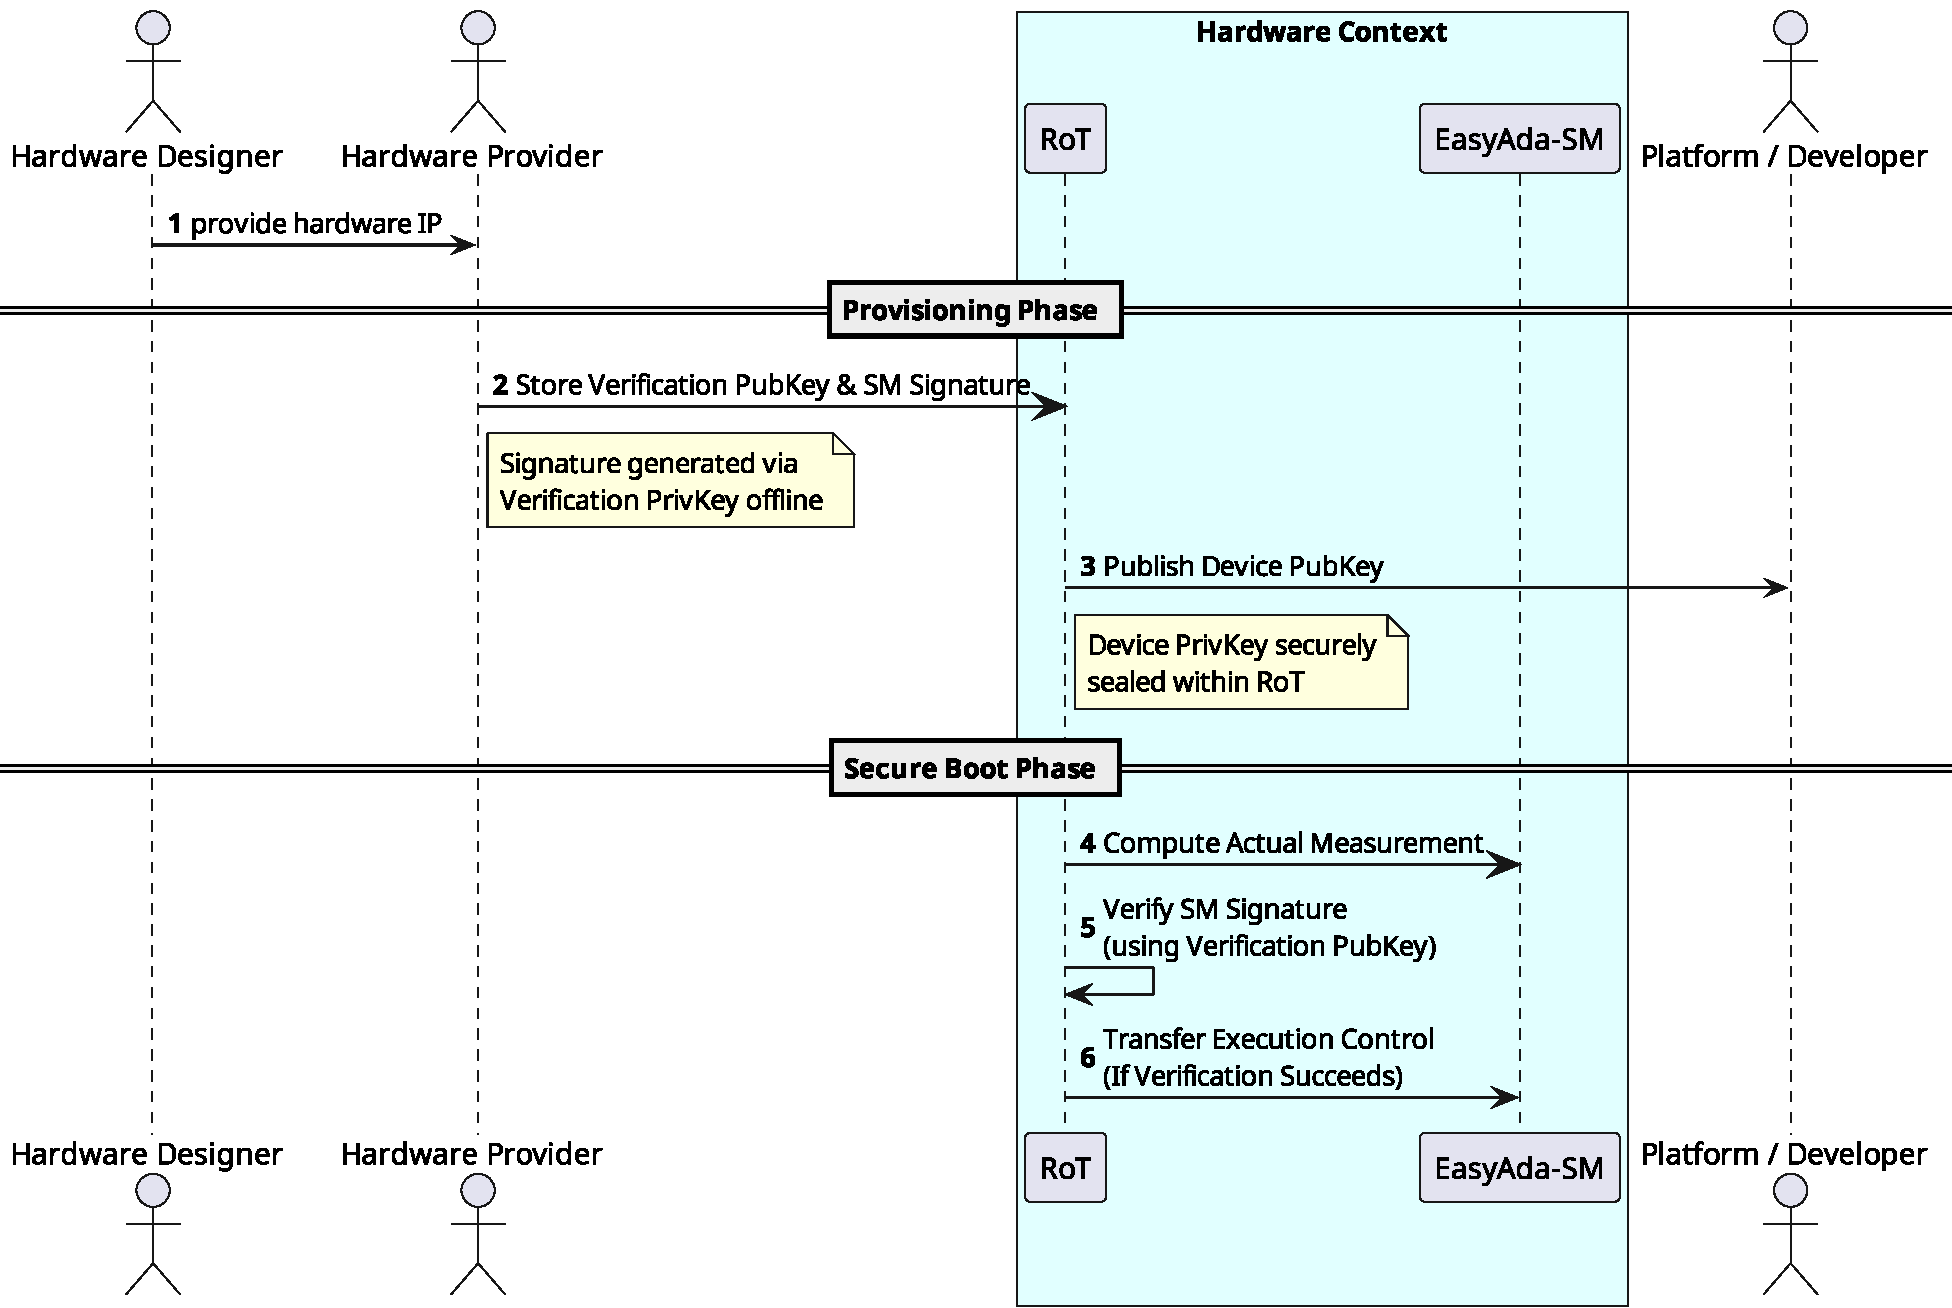
\includegraphics[width=1\linewidth]{key_stage1.pdf}
		\caption{EasyAda-SM签名验证流程}
		\label{key_stage1}
	\end{figure}
	
	SM初始化流程分为两个部分：TSM初始化和SBI运行环境初始化。因为SBI固件被视为不可信或实现可能存在漏洞，因此SM初始化流程由可信的TSM主导。TSM初始化时会首先判断当前硬件环境是否满足部署EasyAda-trust的最低要求，然后清空RoT副本并初始化根安全区域隔离SM自身内存，防止SM在系统运行过程中被运行在更低特权级的不可信组件非法访问和篡改。
	
	完成SM内存隔离后，TSM初始化流程会调用SBI固件实现的接口完成SBI运行环境初始化，然后由TSM完成剩余模块如验证器等的初始化并重新配置SM的陷入入口，确保低特权软件的执行在明确定义的入口点陷入到TSM和SM中，最终转移控制权到下一阶段引导程序或Hypervisor。当TSM初始化完成时，SM已经通过硬件实现了与不可信组件的强制隔离，可以安全进入更低特权级并转移控制权到Hypervisor继续下一阶段初始化。
	
	\begin{figure}[!h]
		\centering		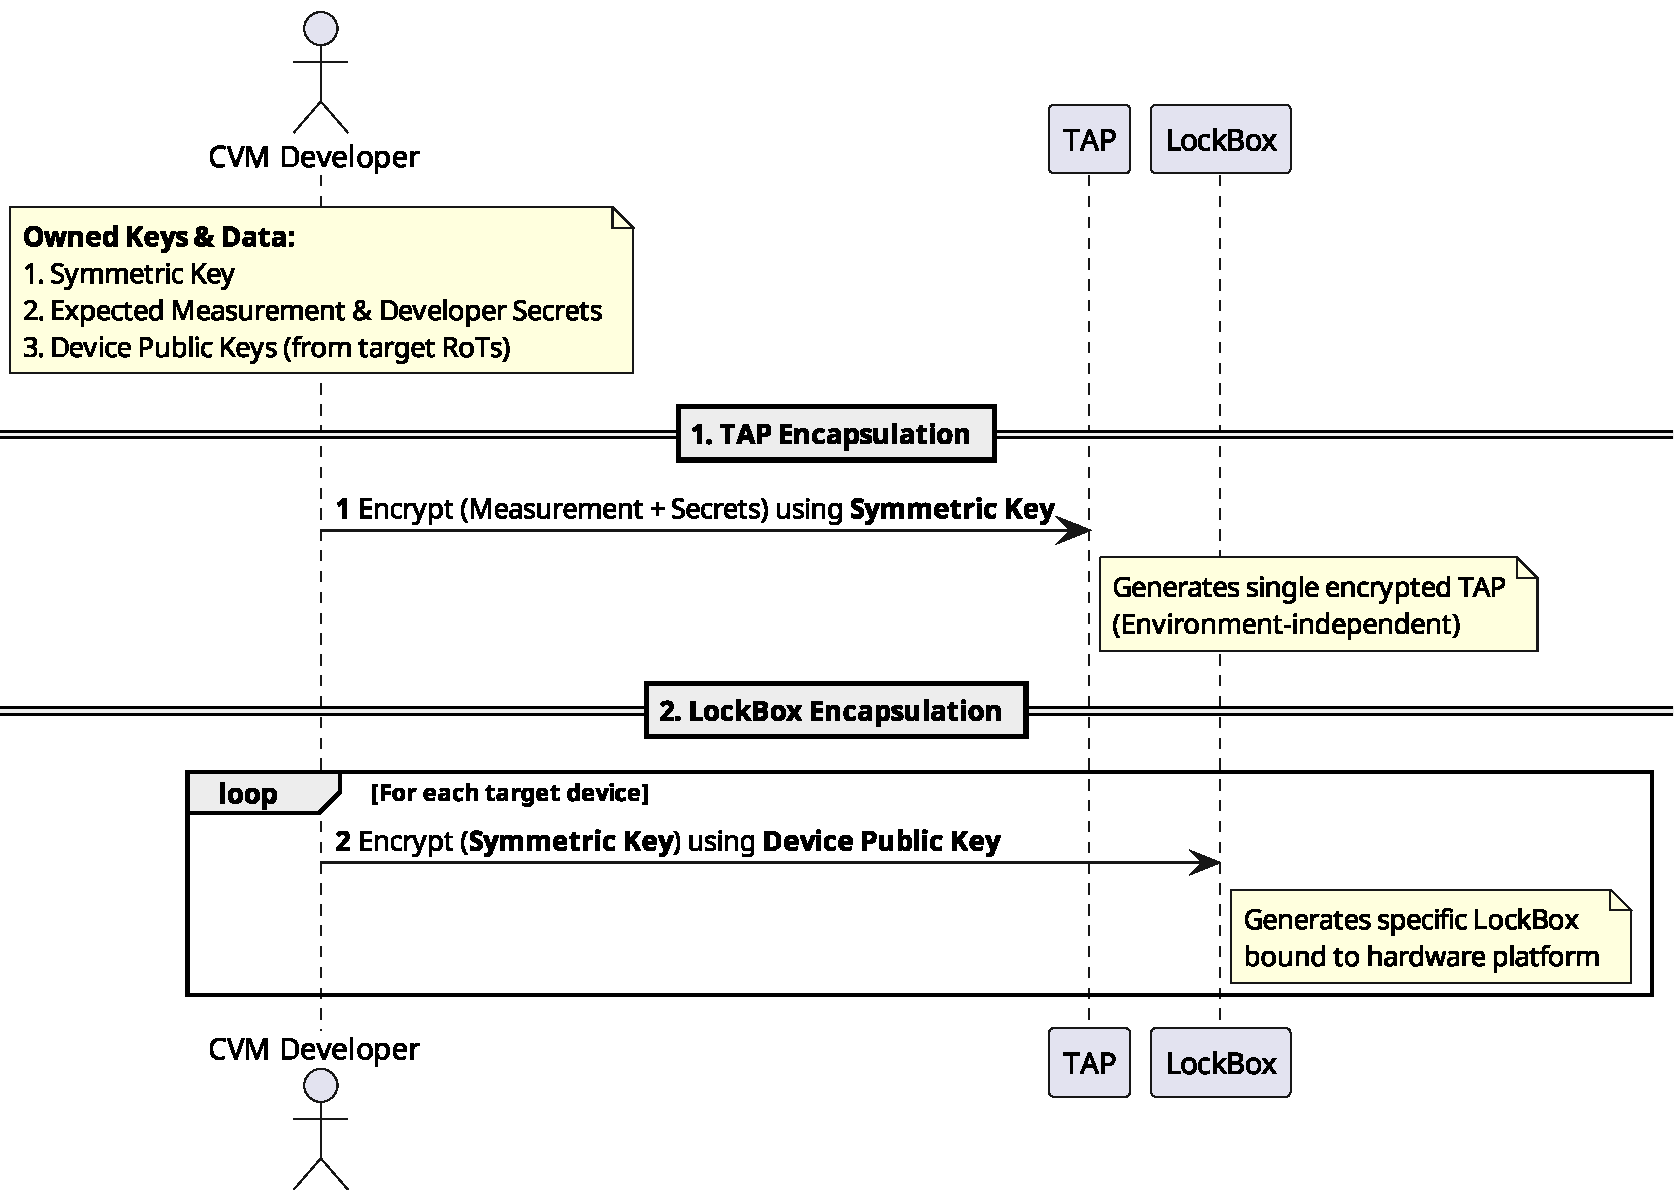
\includegraphics[width=1\linewidth]{key_stage3.pdf}
		\caption{机密虚拟机验证信息封装流程}
		\label{key_stage3}
	\end{figure}
	
	为了支持CVM和硬件环境的本地证明。如图\ref{key_stage3}所示，CVM开发者必须使用开发者提供的密钥对称加密TEE证明载荷（TEE Attest Payload，TAP）文件。该文件用于存储CVM预期度量值和开发者提供的用于加解密敏感I/O数据，代码和参数等的秘密，并且配合一个使用当前设备公钥加密，用于存储加密TAP的对称密钥的锁盒（LockBox）。为了支持在多个设备上进行部署，同一TAP可以关联多个使用不同设备公钥加密的锁盒。
	
	在部署CVM时，SM会将CVM的初始化状态保存到安全内存和hart结构体中并通过验证器模块对关键数据进行度量等到当前度量值，然后使用RoT提供的设备私钥解密锁盒，并使用锁盒中的对称密钥解密TAP，最终得到CVM预期度量值和开发者提供的秘密。如果实际和预期度量值对比成功则验证通过。TSM会将从TAP中解密获得的开发者秘密存储在验证器模块中。CVM可以通过SBI请求获取当前CVM开发者提供的秘密，其它CVM或不可信组件无法窃取或篡改。
	
	\begin{figure}[!h]
		\centering		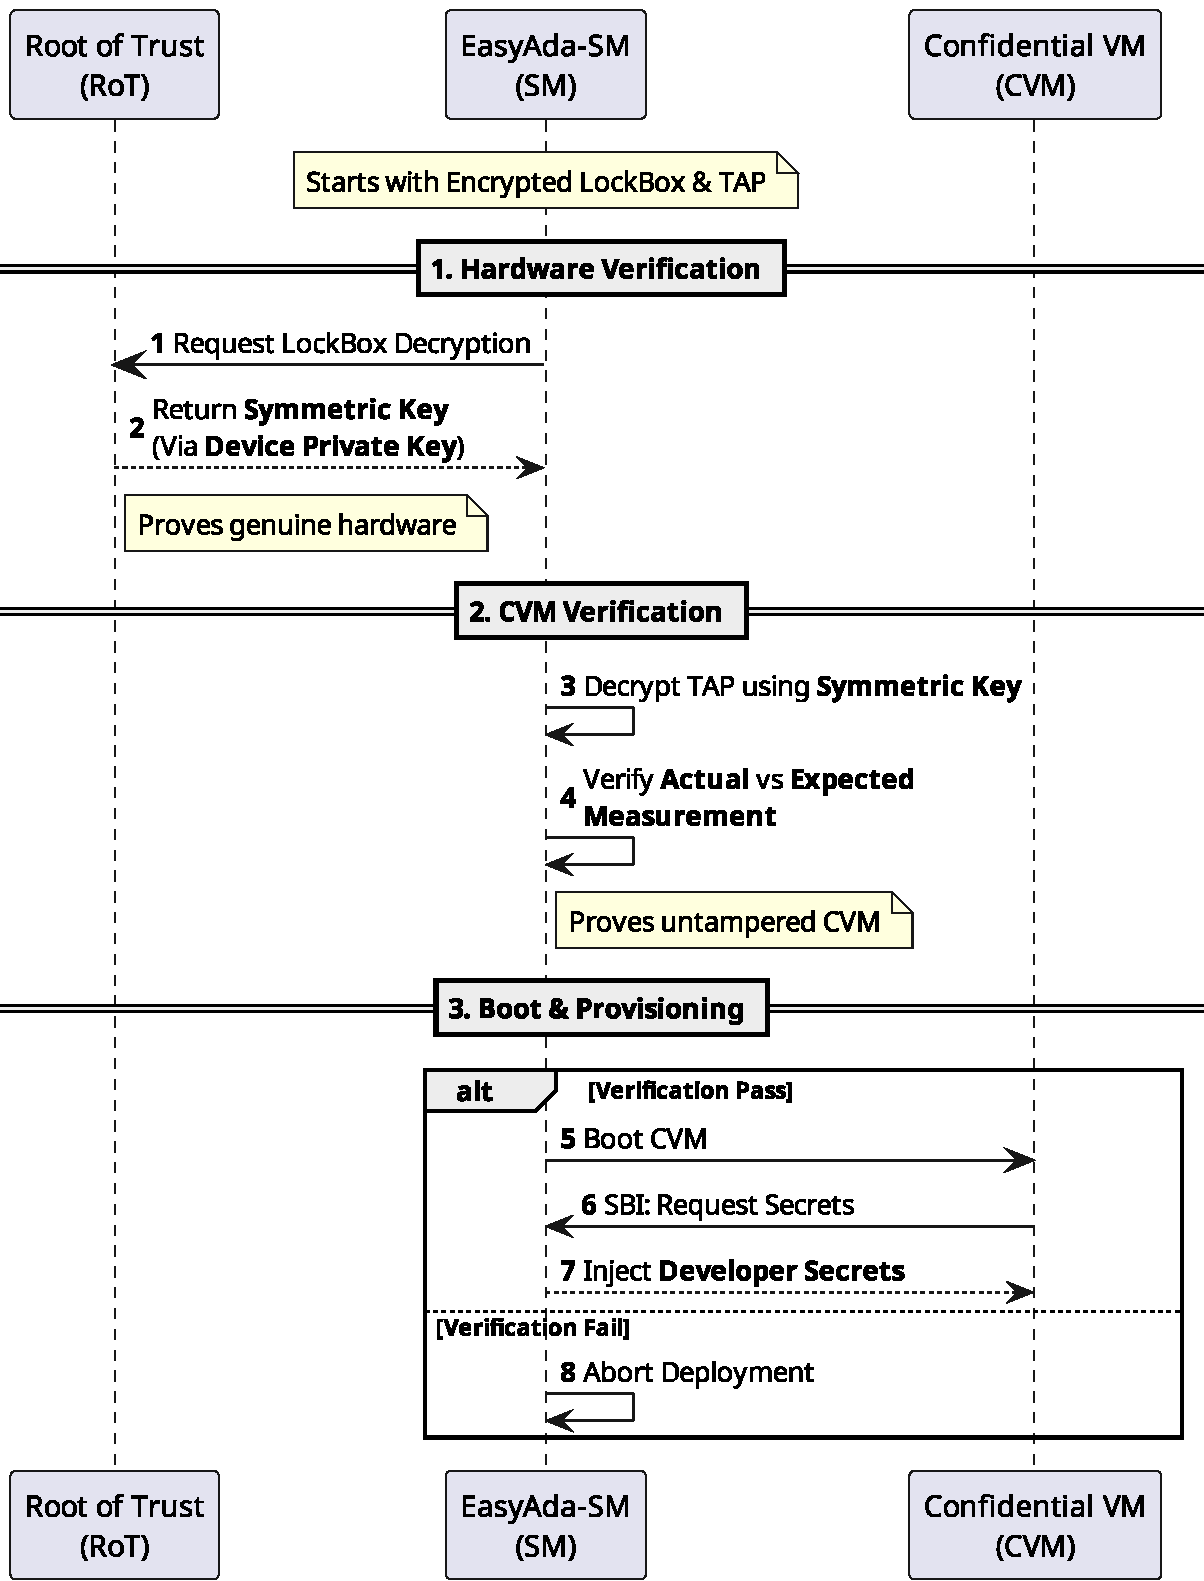
\includegraphics[width=1\linewidth]{key_stage4.pdf}
		\caption{EasyAda-trust中双向验证流程}
		\label{key_stage4}
	\end{figure}
	
	本地证明可以实现CVM与硬件环境的双向证明，如图\ref{key_stage4}所示，因为存储TAP加密密钥的锁盒仅能在持有对应硬件私钥的硬件环境上被正确解密，即使CVM被强行拉起，不可信环境仍然无法获取CVM开发者提供的特定秘密，无法从CVM中解密任何敏感代码或数据；另一方面，任何对TAP，锁盒或者CVM镜像的篡改都会导致最终的度量失败，确保只有可信的，未经过篡改的CVM可以被部署。同时，本地证明与远程证明并不冲突，在具备网络条件的环境上仍然可以使用远程证明验证可信环境。
	
	\section{安全CPU虚拟化实现}
	EasyAda-Hypervisor将虚拟CPU（vhart）抽象为微内核操作系统中的线程进行调度。在其线程控制块(Thread Control Block, TCB)中，除包含标准的通用寄存器状态外，还额外记录了当前虚拟机(VM)的控制寄存器信息，以确保能够精确恢复VM的运行上下文。此外，EasyAda-Hypervisor为每个vhart构建了两个独立的执行上下文：vhart运行线程与vhart服务线程。前者负责存储与调度VM的运行时计算上下文，后者则专职处理VM的异步I/O请求。
	
	为提升系统整体性能，EasyAda-Hypervisor将物理hart静态划分为三类功能区：(1)vhart运行区：主要承担VM及其原生应用的计算任务；(2)vhart服务区：专用于承载vhart服务线程，以异步方式高效响应VM的I/O请求，最大程度降低对VM计算任务的干扰；(3)系统服务区：专用于运行内存管理、进程管理及文件系统等微内核核心系统服务，旨在消除因任务调度抖动而引发的系统性能衰退。
	
	EasyAda-trust在此CPU虚拟化架构的基础上进行了安全维度的扩展，引入了额外的隔离机制，以实现CVM与不可信Hypervisor之间上下文的严格物理隔离。
	
	\begin{figure}[!h]
		\centering		
		\includegraphics[width=1\linewidth]{cpu_area.pdf}
		\caption{EasyAda-trust下hart分区示意图}
		\label{cpu_area}
	\end{figure}
	\subsection{安全上下文管理}
	在EasyAda-trust架构中，底层可信安全监视器(TSM)驱动不介入不可信VM的vhart管理，该职责仍由Hypervisor保留。然而对于CVM的vhart，尽管其宏观调度策略仍由Hypervisor负责，但其核心上下文状态必须由TSM进行机密管理，并对Hypervisor呈现完全的不可见性。Hypervisor仅能通过TSM暴露的有限的CVM生命周期管理接口，间接完成对CVM vhart的调度操作。
	
	如图\ref{cpu_area}所示，EasyAda-trust在原生hart分区机制的基础上，将vhart运行区进一步细分为CVM vhart运行区与不可信VM运行区。两者在架构上的核心差异在于跨执行环境时的上下文切换流程。

	为了规避非必要的上下文保存与恢复开销，EasyAda-Hypervisor将vhart上下文切换机制划分为执行环境内轻量级切换与跨执行环境安全切换两个层级。对于不可信VM，Hypervisor在逻辑上将其上下文解耦为VM侧的VM上下文与Hypervisor侧的vhart运行上下文。两者均各自维护一套完整的状态集合，具体包括：(1)最小架构状态寄存器集合(含通用寄存器及TSM运行时可能变更的控制寄存器)；(2)虚拟化控制寄存器状态；(3)虚拟化功能寄存器状态。由于Hypervisor在自身运行期间不会修改上述(2)与(3)中的寄存器状态，因此VM与Hypervisor之间的上下文切换仅需保存集合(1)的信息即可。然而，在不同VM实例之间进行切换时，则必须完整保存并清理涵盖(1)、(2)、(3)在内的全量上下文信息。为此，Hypervisor通过vhart运行线程统一管理这两类逻辑上下文状态。
	
	相比之下，CVM的上下文切换呈现出以下显著的安全特征：
	\begin{enumerate}
		\item 扩展的上下文保护范围：鉴于CVM对Hypervisor处于完全不信任状态，除上述三类基础上下文信息外，TSM还必须额外切换并保护机器模式(M-Mode)与硬件虚拟化监管者模式(HS-Mode)的控制寄存器(例如中断与异常委派状态寄存器等)。
		\item 物理内存视图的严格隔离：CVM与Hypervisor分别运行于相互隔离的物理内存视图中。在触发上下文切换时，TSM必须动态重配置底层安全硬件(如PMP)，以维持安全内存与不可信组件之间的物理隔离边界。
		\item 执行流的安全阻断与切换：CVM与Hypervisor的执行流彼此互斥。在处理特定异常(如MMIO访问异常)而触发执行流切换时，必须确保Hypervisor无法窥探或获取任何属于CVM及TSM的上下文残余信息。
	\end{enumerate}
	
	针对上述特征，EasyAda-trust将CVM相关的上下文严格划分为“不可信vhart上下文”与“机密vhart上下文”两类。前者负责暂存Hypervisor侧vhart运行线程的全部状态，后者则专用于安全存储CVM的全量状态。两者均涵盖所有通用寄存器以及VS/HS/M态系统控制寄存器；若底层硬件使能了浮点或向量指令扩展，还需额外保护浮点或向量处理单元的上下文信息。
	
	为缓解CVM与Hypervisor间频繁交互带来的性能损耗，若当前hart控制流未跨越信任边界，则仅执行轻量级上下文切换；反之，则必须执行完整的安全上下文切换流程。
	
	轻量级上下文切换：当当前hart从Hypervisor或CVM陷入TSM执行特定服务时，由TSM直接原地完成请求处理。在此过程中，hart仅需临时保存当前执行环境的通用寄存器，待TSM处理完毕后直接恢复。由于该过程不涉及执行环境的越界切换，因此无需动态重构物理内存保护视图，切换开销极小。
	
	安全上下文切换：当当前hart必须在Hypervisor与CVM之间转移控制权时，需严格遵循CVM管理模块的状态机约束。在完成必要参数的安全校验与传递后，TSM会将当前全量上下文状态加密(或隔离)存储至对应的vhart结构中，随后彻底清理当前物理环境的残余寄存器状态，最后加载目标执行环境的上下文，从而完成执行流的安全迁移。在执行目标指令前，TSM必须重新配置安全硬件以切换物理内存视图。具体而言，当控制流由不可信vhart切换至机密vhart时，TSM会授权当前hart访问除安全监视器(SM)自身内存外的所有关联安全区域及不可信内存(此时依靠二阶段页表机制，TSM足以严密管控CVM的最终物理寻址能力)；反之，当控制流由机密vhart切回不可信vhart时，TSM将立刻剥夺当前hart对所有安全区域的物理访问权限。

	\subsection{安全异常处理}
	如第\ref{CVM管理模块_exception_sec}节所述，EasyAda-SM通过Rust语言的静态内存检查机制，从编译源头消除了因不安全内存访问而导致的敏感数据泄漏隐患，并凭借构造-处理-析构的规范化生命周期模型，严格界定了各项处理服务所能触达的资源边界。与此同时，TSM在架构设计上刻意摒弃了向不可信组件内存空间写入数据的能力，从根本上阻断了机密数据向不可信域泄漏的物理路径。
	
	然而必须强调的是，尽管TSM在底层机制上保障了不同处理器与执行流之间的物理安全，但CVM内部的客户操作系统仍需肩负起正确调用TSM安全接口的责任。例如，当TSM为CVM分配不可信的共享物理内存以实现I/O半虚拟化时，由于该内存区域暴露于不可信环境中，TSM本身无法为其提供端到端的机密性与完整性保障。因此，CVM必须在应用层或客户内核层，自主引入必要的密码学加解密与度量校验机制，以确保共享数据的流转与使用严格符合安全预期。
	
	\section{安全内存虚拟化实现}
	内存虚拟化主要涵盖VM运行时内存、设备MMIO区域以及用于I/O半虚拟化的共享内存的二阶段页表映射。二阶段页表的根页表基址作为VM配置的核心信息，被保存在vhart运行线程的上下文中。EasyAda-Hypervisor按照以下标准流程构建并维护二阶段页表：（1）用户态VMM解析当前VM的配置文件（如FDT），计算VM所需的运行时物理内存规模（不包含MMIO区域），并通过系统服务申请相应的物理内存页；（2）依据配置文件约束，将VM的Kernel、FDT等关键镜像加载至满足对齐要求的物理地址中；（3）依据配置文件构建GPA至HPA的映射关系，由运行在内核态的Hypervisor驱动创建初始的二阶段页表，并将其基址存入对应的vhart运行线程上下文中。
	
	MMIO区域的映射主要服务于设备直通（Device Passthrough）场景。在创建VM时，运行于内核态的Hypervisor驱动会解析配置文件中的物理设备信息，基于GPA与HPA的映射关系，将目标物理设备的MMIO区域直接映射至VM的独立地址空间中。此外，Hypervisor还会将该硬件设备的物理中断号注册并绑定至目标VM，以确保后续的虚拟中断注入机制能够正确触发，从而保障VM对直通设备的正常访问与中断响应。
	
	共享内存映射主要服务于基于半虚拟化技术的虚拟设备管理。其初始化过程采用按需分配机制：当VM在系统运行过程中首次访问虚拟设备的MMIO区域（GPA）并触发异常时，内核态的Hypervisor驱动将拦截该异常。经与虚拟设备注册信息匹配确认后，若该GPA属于合法的虚拟设备MMIO范围，Hypervisor驱动将切换至vhart运行上下文，并在用户态向微内核系统服务申请对应的物理共享内存。随后，由Hypervisor驱动在内核态完成该共享内存到VM二阶段地址空间的映射，并从异常处理返回，恢复VM的继续执行。在EasyAda的底层实现中，共享内存被抽象为UNIX风格的文件对象，该文件的所有权归属于vhart运行线程，并在常规架构下被映射至vhart服务线程中，以支撑高效的异步I/O交互。
	
	在EasyAda-trust架构中，针对不可信VM的内存虚拟化流程保持原貌，但将CVM的内存虚拟化控制流与不可信Hypervisor进行了深度解耦。具体而言，Hypervisor仅保留宏观物理层面的安全区域创建与共享内存分配权限，而核心的受保护内存/设备分配权及二阶段页表映射逻辑，则全权由受信任的TSM接管。
	
	\subsection{基于TSM接口的安全区域生命周期管理}
	如前文所述，安全区域的具体物理抽象、隔离机制与内部内存管理层已在EasyAda-SM固件中实现并封装。在EasyAda-trust架构中，Hypervisor无需感知安全区域底层的PMP配置与物理鉴权细节，而是作为上层资源调度者，通过TSM对外暴露的安全管理扩展接口，完成CVM所需核心物理内存的动态构建、分配与回收。
	
	\subsubsection{安全区域的动态创建触发}
	在系统运行期，当Hypervisor判定需为CVM扩充安全环境时，将主动通过微内核系统服务申请满足连续性约束的物理内存或物理外设的MMIO区域。随后，Hypervisor将该物理地址空间作为参数，通过特权级调用触发TSM的安全区域创建接口。在此协同流程中，Hypervisor仅负责宏观物理资源的供给与上层业务的无中断调度，而核心的基于可信硬件配置的合法性校验、物理属性确权以及底层硬件强隔离机制，均交由EasyAda-SM在极高特权级下透明完成。一旦TSM返回创建成功信号，Hypervisor即在内部资源表中将该物理区间标记为“不可见”，彻底剥离不可信环境对该区域的寻址能力。
	
	\subsubsection{基于单次请求的特权提升与按需分配}
	在初始化阶段，Hypervisor首先遵循标准VM的创建流程，为目标VM分配常规的内存与设备资源，并完成其基础逻辑架构的初始配置。当业务场景需要将该标准VM提升为CVM时，Hypervisor不再精细化介入底层安全资源的调度过程，而是仅通过一次独立的SBI请求，向TSM下达特权提升与转换指令。
	
	TSM在截获该SBI请求后，将全权接管后续的安全资源配置工作：其会自主从当前已就绪的全局安全区域池中，为该CVM按需划拨容量匹配的内存型安全区域（用于承载CVM镜像与二阶段页表等核心元数据），并尝试预分配必需的设备型安全区域。待该CVM完成本地度量证明并被系统确认为绝对可信后，由TSM独立执行实质性的安全区域物理分配与二阶段页表的安全重映射，从而以最小的Hypervisor交互代价完成了CVM的资源构建。
	
	\subsubsection{安全区域的安全回收调度}
	当系统面临物理内存或外设资源瓶颈，抑或CVM生命周期终止时，Hypervisor作为全局资源管理者，可向TSM发起主动的资源回收调度请求。针对内存型安全区域，Hypervisor请求TSM扫描并释放特定或空闲的安全区域；针对设备型安全区域，Hypervisor需显式提供目标设备的MMIO地址以请求解绑。TSM在底层安全释放硬件隔离限制并完成必要的数据擦除后，会将物理控制权交还。Hypervisor接收到释放成功的确认后，重新将该物理内存或设备MMIO区间纳入不可信系统的可用资源池中，从而形成完整的资源调度闭环。

	\section{安全I/O虚拟化实现}
	EasyAda-Hypervisor原生支持三种I/O虚拟化技术：（1）全虚拟化：用于模拟逻辑简单或安全性要求较高的基础组件（如串口与中断控制器等）；（2）半虚拟化：用于支撑大吞吐量I/O数据流的设备（如网卡、块存储设备等）；（3）设备直通：用于管理驱动逻辑复杂或具备专有计算能力的硬件外设（如AI硬件加速器等）。
	
	在原生架构中，VM的设备初始化被设计为VM无感的被动触发流程，旨在最大程度减少对Guest OS代码的侵入。系统采用静态分区与动态分配相结合的硬件发现机制，其完整流程涵盖三个阶段：（1）系统静态配置阶段：硬件供应商提供包含全局视角的FDT，应用开发者依此划分直通设备，并在VM的专属硬件配置文件中建立静态绑定关联；（2）VM初始化阶段：Hypervisor解析该配置文件，若存在匹配的直通外设则将其逻辑分配给目标VM，否则降级为全虚拟化模拟；（3）首次访存触发阶段：设备被分配后，VM的首次MMIO访问将触发缺页异常并陷入至Hypervisor。针对全虚拟化设备，由Hypervisor直接接管处理；针对半虚拟化设备，Hypervisor将建立不可信共享内存及主从异步事件通知信道（VM主动发起访问触发事件，vhart服务线程异步处理后通过中断注入返回结果）；针对直通设备，则由Hypervisor完成物理MMIO至GPA的最终映射，交由VM自主完成驱动初始化。
	
	针对CVM的高安全需求，EasyAda-trust在复用上述全虚拟化与半虚拟化基础路由逻辑的同时，重点对设备直通与数据通道进行了深度的安全扩展。安全设备的生命周期依然由Hypervisor驱动宏观调度，但其底层鉴权与物理隔离全权由TSM把控。本节将重点阐述EasyAda-trust如何保障CVM使用I/O设备过程中的全链路安全性。

	\subsection{安全直通设备生命周期管理}
	EasyAda-trust对安全外设实施“主机分配，TSM鉴权”的协同管理机制。在系统构建阶段，硬件供应商需在底层固化Trusted FDT，同时应用开发者需提供CVM专用的虚拟硬件配置文件。这一机制将复杂的运行时设备发现转化为静态的密码学信任链校验，极大降低了安全架构的动态攻击面。
	
	在标准VM创建阶段，Hypervisor仍遵循常规逻辑进行设备初始化与逻辑映射，但此时VM并不具备对该物理外设的实际读写权限。当Hypervisor请求将该普通VM提升为CVM时，TSM将介入并执行严格的设备鉴权：其将CVM配置文件中声明的外设与底层Trusted FDT进行交叉比对。若匹配成功且被标记为可信，TSM将为该设备分配专属的设备型安全区域；若匹配失败，则强制将该MMIO区域降级回退为全虚拟化处理，防范Hypervisor恶意挂载仿冒外设。
	
	在CVM运行期，当其首次访问MMIO区域并陷入至TSM时，TSM将依据MMIO地址的属性类别实施安全路由：若属全虚拟化设备，则将请求转换为标准MMIO拦截事件并转发至Hypervisor侧处理；若属半虚拟化设备，则转换为不可信共享内存映射请求交由Hypervisor调度；若属已鉴权的安全直通设备，TSM将在底层安全构建物理MMIO至CVM地址空间的二阶段页表映射，随后将控制权交还CVM以完成原生的设备初始化。

	\subsection{基于IOPMP的设备侧防DMA攻击隔离}
	仅在CPU侧通过MMU/PMP隔离MMIO空间，仍无法抵御具备DMA（Direct Memory Access）能力的恶意外设越权访问安全内存。为此，EasyAda-trust引入了IOPMP硬件扩展，从总线级构建外设访存的物理安全网关。在硬件开发阶段，供应商需为所有硬件设备静态分配唯一源标识符（Source ID）。
	
	在系统启动初始化阶段，TSM会默认接管全局IOPMP控制器，并为所有已注册的SID创建并绑定初始的不可信MD。该不可信MD的基础访问控制策略被严格设定为允许访问不可信物理内存，但直接屏蔽并拦截对任何受保护的安全区域的寻址请求。所有未被显式提升为安全设备的外设，其SID均被默认约束于此不可信MD内，从而确立了系统初始阶段防范DMA攻击的默认拒绝（Default-Deny）物理隔离基线。因为所有设备共享相同的不可信内存视图，所以共享同一个不可信MD。
	
	在系统运行期，伴随CVM生命周期的演进，每当Hypervisor通过TSM成功创建一个全新的安全区域时，TSM将立即触发全局IOPMP状态同步机制。具体而言，TSM会遍历并修改不可信MD的内部规则，将针对该新增安全区域的限制访问条目动态注入其中。这一严格的实时同步策略确保了即使安全内存是动态分配与衍生的，所有驻留于不可信环境的常规外设亦无法通过DMA途径对其进行非法的探测、读取或篡改。
	
	当Hypervisor请求将特定物理外设提升为安全设备以供CVM独占使用时，TSM首先校验该设备SID对应的可信硬件配置属性。鉴权通过后，TSM会为该设备分配一个处于隔离状态的可信MD。唯有当该安全设备被实质性地挂载并分配给目标CVM时，TSM才会动态更新该可信MD，将当前CVM所关联的所有内存型安全区域的授权条目注入其中，并将该设备的SID从不可信MD解绑，转而与该可信MD强绑定。至此，IOPMP硬件强制限定该直通设备仅能对其从属CVM的受保护内存发起DMA操作，不仅防范了外部入侵，亦从物理总线层面彻底杜绝了设备内部敏感数据向不可信内存泄漏的风险。
	
	反之，当CVM生命周期终止并触发安全设备释放时，TSM将立即重置并安全擦除该设备所对应可信MD中的所有授权规则。在Hypervisor请求回收该外设资源时，TSM会将其SID重新降级并绑定至不可信MD，从而在确保物理安全的界限下，完成硬件外设的归还与状态复原。

	\subsection{I/O数据平面安全与端到端保护}
	确立了设备控制平面的物理隔离后，必须进一步保障I/O数据平面的机密性与完整性。机密应用（如部署于CVM中的AI推理引擎）是高价值I/O数据（如AI模型权重与用户输入）的核心消费者。

	I/O数据保护的基石在于密钥的安全供应。在系统启动阶段，CVM与底层硬件环境之间将执行双向本地证明。确认环境可信后，TSM利用RoT内置的设备私钥解锁受保护的锁盒（Lockbox），获取对称密钥并进一步解密目标CVM提供的TAP，从而安全提取出开发者预置的机密素材（Secrets）并暂存于TSM内部。在CVM运行时，Guest OS可通过安全的SBI请求，从TSM处按需获取相应的开发者密钥或会话密钥。

	获取密钥后，CVM需针对不同类型的I/O通道采取差异化的安全策略：
	\begin{enumerate}
		\item \textbf{安全直通设备的数据流}：得益于PMP与IOPMP构建的双向物理隔离屏障，不可信组件（包括Hypervisor）无法以任何形式窥探直通外设的MMIO与DMA区域。因此，机密应用可直接以明文形态向安全设备（如直通硬件加速器）下发控制指令与AI模型参数，而无需承受额外的软件加解密性能损耗。
		\item \textbf{半虚拟化设备的数据流}：对于基于不可信共享内存构建的半虚拟化信道（如网络与磁盘I/O），数据必须穿越不可信Hypervisor的控制边界。在此场景下，CVM必须利用预先供应的对称/非对称密钥，在软件栈顶层实施端到端的密码学加解密与报文认证码校验，坚决拒绝接收及执行任何被Hypervisor篡改、重放或伪造的I/O载荷。
	\end{enumerate}

	\section{机密异构计算环境实现}
	
	EasyAda-trust一个重要的目标是保障用户AI模型和敏感数据的机密性和完整性。该目标可以进一步细分为两个目标：
	\begin{enumerate}
		\item 保障用户运行环境的可信和隔离：为了保护用户AI模型，CVM仅能在可信的硬件环境上对用户模型进行解密和部署，并且由EasyAda-trust确保CVM运行环境与不可信组件的隔离。
		\item 保障用户I/O数据的机密性和完整性：为了确保用户敏感数据不被窃取或篡改，EasyAda-trust需要对用户I/O数据采取必要的加密和校验，并确保用户模型使用硬件加速器过程中的安全。
	\end{enumerate}
	
	同时，EasyAda-trust为了增强系统的可扩展性，需要实现硬件加速器在不同执行环境间的复用，为了实现以上目标，EasyAda-trust实现了专用的硬件加速器管理CVM，并通过I/O半虚拟化技术实现硬件加速器在不同执行环境间的复用。下面将详细介绍EasyAda-trust如何实现机密异构计算环境。
	
	\subsection{硬件加速器的保护}
	
	为了确保CVM使用硬件加速器过程中的安全性，Hypervisor必须显式将硬件加速器提升为安全设备，TSM在加速器管理CVM启动时，会检查并尝试分配安全设备，只有经过验证的安全硬件加速器可以映射到CVM的地址空间中进行管理。同时，硬件加速器使用的内存缓冲区由加速器管理CVM内的驱动从当前CVM的安全内存中进行分配，不可信组件无法访问安全的内存缓冲区和MMIO区域。

	\subsection{加速器管理CVM初始化}
	\begin{figure}[!h]
		\centering		
		\includegraphics[width=1\linewidth]{acccvm_pmp.pdf}
		\caption{引入安全设备后的CVM安全内存视图}
		\label{acccvm_pmp}
	\end{figure}

	在未引入CVM的架构下，EasyAda-Hypervisor为了实现对现有驱动的复用，避免增大微内核操作系统的攻击面，会在启动阶段将硬件加速器的MMIO地址透传到硬件加速器管理VM中，由该VM加载驱动并完成硬件加速器初始化，后续通过I/O半虚拟化技术（如VirtI/O协议）实现硬件加速器在VM间以及host间的时分复用。
	
	加速器管理CVM的创建与其他CVM类似，在创建加速器管理CVM前，Hypervisor需要主动将可信的硬件加速器提升为安全硬件，因为提升时机由EasyAda-Hypervisor决定，应当由其自身确保无任何组件正在访问硬件加速器，避免访问流程的异常中断。当硬件加速器被提升为安全设备后，不可信组件无法访问硬件加速器的MMIO区域，
	
	
	接下来由Hypervisor负责创建CVM，在TSM为CVM分配安全设备时，会同时为硬件加速器创建授权MD用于授予当前硬件加速器访问安全区域的能力，因为端侧硬件加速器多以协处理器的形式集成在SoC中，因此其数据缓冲区需要动态进行分配，为了降低IOPMP管理的开销，TSM配置IOPMP授权硬件加速器访问加速器管理CVM关联的所有安全区域以确保可以正常访问动态数据缓冲区，因为配置DMA时会通过IOMMU或TSM软件翻译IPA为物理地址，避免了硬件加速器因为DMA配置错误写入其它安全内存中。隔离完成后，不可信组件无法访问硬件加速器的MMIO区域，硬件加速器也无法写入不可信的内存区域。
	
	加速器管理CVM创建成功后，如图\ref{acccvm_pmp}所示，此时加速器管理CVM是除TSM外唯一可以访问硬件加速器软件实体。当加速器管理CVM实际运行时，需要按照安全启动流程，CVM从TSM获取开发者密钥并对开发者提供的AI模型和参数进行解密和部署，并对不可信的半虚拟化和全虚拟化设备进行初始化。	

	加速器管理CVM创建成功之后，可以直接对其上的机密应用提供服务。如果需要与不可信环境间进行复用，则需要与请求使用硬件加速器的不可信组件建立信道，下面将介绍信道建立的过程。
	
	\subsection{建立信道}
	
	加速器管理CVM其它组件均通过I/O半虚拟化技术——VirtI/O协议实现硬件加速器的时分复用。
	
	虚拟设备的发现在开发是通过静态的硬件配置文件如FDT文件静态完成，EasyAda-trust应用开发者需要根据硬件供应商提供的可信物理硬件配置完成设备静态分区，并在加速器管理CVM的硬件配置文件中预留内存区域用于建立映射共享内存。
	
	加速器管理CVM会对设备进行初始化，当访问到预留的内存区域时会陷入TSM，由TSM检查MMIO区域类型后，将共享内存申请请求转发到EasyAda-Hypervisor处理。EasyAda-Hypervisor负责完成共享内存分配并返回地址给TSM，由TSM完成共享内存到CVM地址空间的映射以及CVM上下文的恢复，并准备进行驱动后端初始化。同时，EasyAda-Hypervisor会标记该共享内存为虚拟硬件加速器设备区域，等待映射到驱动前端中。
	
	当不可信VM尝试初始化虚拟硬件加速器时，会陷入到EasyAda-Hypervisor中，由EasyAda-Hypervisor将会获取之前加速器管理CVM申请的共享内存，并将其映射到请求方VM对应的虚拟设备地址中。之后VM和加速器管理CVM可以通过该共享内存完成数据交换，由TSM和EasyAda-Hypervisor转发和注入中断进行I/O请求通知和回复。EasyAda-trust并不要求加速器管理CVM和请求方VM的初始化时序，双方可以由任意一方进行初始化并完成共享内存的申请和标记，EasyAda-trust不感知实际的进一步的协议交互和信道建立流程，通信双方可以基于共享内存，通过轮询或中断完成通信协议的初始化。

	\section{本章小结}
	本章详细论述了基于微内核的可信虚拟化方案的工程实现，重点阐述了如何适配EasyAda-Hypervisor以实现对CVM的安全管理与资源虚拟化 。在CPU虚拟化方面，方案通过扩展EasyAda-Hypervisor的hart分区架构，引入了机密与非机密 vhart运行区，并利用TSM接管CVM的两阶段安全上下文切换流程，确保了CVM的CPU状态对不可信Hypervisor完全隐匿。在内存与I/O虚拟化层面，方案将安全资源的直接控制权从EasyAda-Hypervisor中剥离，确立了由Hypervisor负责物理内存分配、设备发现与宏观生命周期调度，进而委托TSM完成安全区域动态构建、二阶段页表隔离映射及安全设备鉴权配置的职责解耦机制。此外，针对端侧异构计算需求，方案利用EasyAda-Hypervisor辅助建立不可信共享内存通信信道，成功实现了专用硬件加速器管理CVM的安全部署与跨环境复用。综上所述，本章通过对EasyAda-Hypervisor 实施职责解耦与非侵入式安全扩展，在充分复用微内核统一资源管理优势的同时，为CVM提供了一个高安全、高可靠的可信虚拟化运行底座。
	
	\chapter{系统测试与分析}
	\section{测试目标}
	本章旨在对基于微内核的可信虚拟化架构EasyAda-trust及其核心组件EasyAda-SM进行系统性的定量评估与安全性验证。评测过程重点围绕以下四个核心科学问题展开：
	1.生态兼容性：采用Rust语言重构并引入安全区域抽象的EasyAda-SM是否能够以尽可能小的代价兼容现有RISC-V TEE生态系统？
	2.基础性能开销：消除不安全内存访问并引入强隔离机制后，EasyAda-trust在核心计算任务中引入的额外性能损耗是否在可接受范围内？

	
	\section{测试软硬件环境}
	
	鉴于当前RISC-V硬件生态的客观限制，目前量产的RISC-V商用芯片在安全特性上存在明显的路线分化：面向端侧的芯片普遍支持PMP和IOPMP扩展，但是缺乏对H扩展的支持；而面向高性能计算场景的芯片虽然支持H扩展，但是通常集成较复杂的IOMMU和高级中断架构（AIA）。然而，这类复杂组件高昂的硬件面积开销及基于总线事务的中断延迟抖动，使其难以在成本与实时性敏感的嵌入式SoC中广泛落地。因此，
	
	\section{EasyAda-SM可拓展性测试}
	参考EasyAdaZone的实验设计\citess{rubbish}。EasyAda-trust基于EasyAda-SM实现了兼容Penglai和Keystone的Enclave管理模块以验证EasyAda-SM可拓展性。该测试在极小化代码修改的前提下，除引导程序与SM外完全复用了既有Keystone与Penglai框架中的全量组件。复用范围涵盖宿主机用户态接口、编译工具链、软件依赖库、测试用例以及受保护侧的TA，并以Linux（内核版本4.15）作为Host OS。在性能评估方面，本文选用Coremark和RV8 benchmark作为基准测试集，并以原生Linux环境的执行表现作为对比基线。
	
	\subsubsection{Coremark测试套}
	如图\ref{coremark}所示，所有测试结果均以非EasyAda-SM环境的原生Linux环境（Native Linux）的得分为基线（100\%）进行归一化处理。实验数据表明，在引入EasyAda-SM后，系统的计算性能得到了极大的保留。在Linux、Keystone与Penglai三种工作负载下与未引入安全防护的原生环境相比，EasyAda-SM环境的相对性能衰减均被严格控制在2\%以内。
	
	因为Coremark属典型的CPU密集型载荷，其执行路径高度集中于用户态及Enclave内部。由于本文所提架构充分利用了RISC-V硬件级的PMP扩展，安全隔离校验在微架构流水线中隐式完成，且Rust语言的内存安全检查均发生在编译期。因此，只要未触发跨特权级的上下文切换，EasyAda-SM不会对核心运算流水线引入任何运行时开销。
	\begin{figure}[!h]
		\centering
		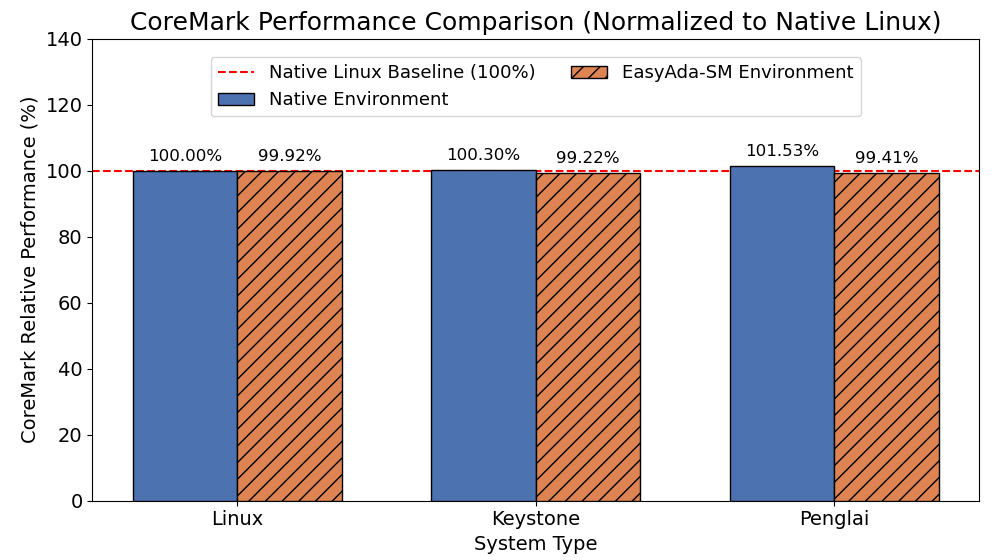
\includegraphics[width=1\linewidth]{coremark.png}
		\caption{原生环境与EasyAda-SM环境下Coremark的对比测试}
		\label{coremark}
	\end{figure}
	
	\subsubsection{RV8基准测试套}
	为了进一步探究EasyAda-SM环境在面对具有不同指令分布与复杂访存行为特征的应用时的性能表现，本文引入了RV8 benchmark测试集。该测试集包含AES（加密）、Miniz（数据压缩）、Primes（素数计算）、Bigint（大数运算）以及Norx（认证加密）等五项典型负载。所有测试结果均以原生 Linux环境为归一化基准（1.0）。
	
	\begin{figure}[!htb]
		\centering
		\subfloat[Penglai对比测试结果]{
			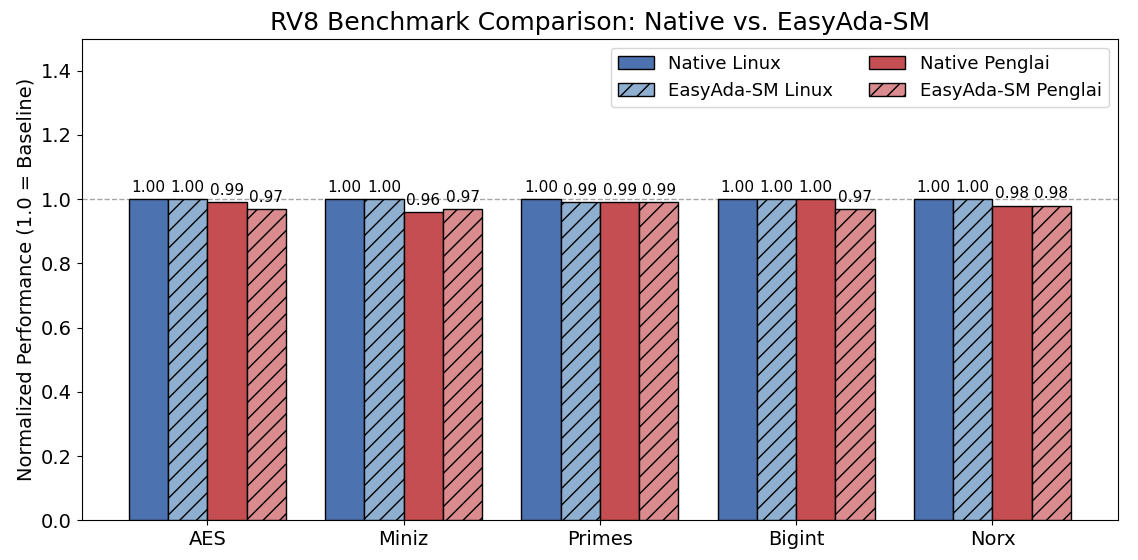
\includegraphics[width=1\linewidth]{penglai_rv8mark.png}
			\label{penglai_rv8mark}
		}
		\hfill
		\subfloat[Keystone对比测试结果]{
			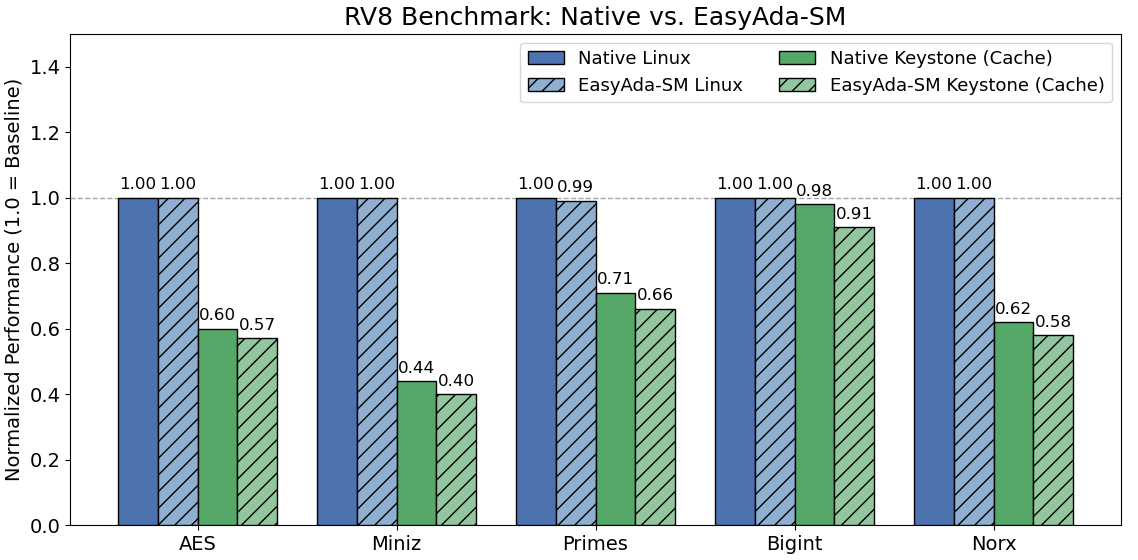
\includegraphics[width=1\linewidth]{keystone_rv8mark.png}
			\label{keystone_rv8mark}
		}
		\caption{原生环境与EasyAda-SM环境下RV8 benchmark测试结果对比}\label{rv8mark}
	\end{figure}
	
	如图\ref{penglai_rv8mark}所示，在未显式开启微架构侧信道防御的Penglai轻量级Enclave场景下，Penglai在原生环境和EasyAda-SM环境下均展现出卓越的执行效率，各项负载归一化得分均不低于0.96。以访存密集型的Miniz为例，二者得分分别为0.96与0.97，证实了引入基于Rust的EasyAda-SM及安全区域内存抽象后，系统的额外性能损耗被严格控制在1\%至2\%的极小区间内，底层特权级调度对上层复杂业务逻辑的执行干扰极微。
	
	然而，在适配Keystone框架的测试中，系统性能呈现出显著的差异化衰减：如图\ref{keystone_rv8mark}所示，Miniz与AES的相对性能分别断崖式下跌至约0.40与0.57，而计算密集型的Bigint受影响较小，分析可能是因为Keystone为防御缓存侧信道攻击，在物理层面强制启用了硬件缓存分区隔离机制，严格限制了Enclave可用的末级缓存路数，导致高度依赖数据局部性的算法缓存缺失率剧增。在未启用缓存分区的环境中，横向对比原生环境和EasyAda-SM环境可知，EasyAda-SM引入的绝对软件开销仅为3\%至7\%，这一处于合理区间的微小性能折损，主要源于EasyAda-SM模块化分层抽象所导致的底层执行链路延长。

	
	综合上述交叉验证与基准测试结果表明，本文提出的基于Rust构建的内存安全监视器EasyAda-SM在确立坚实底层信任根的同时，兼具高度的执行效率与架构弹性。具体而言，在纯计算密集型负载下，得益于PMP机制的流水线隐式校验以及Rust语言编译期的零成本抽象特性，该安全架构所引入的运行时额外开销与原生实现相比趋近于零。

	\section{EasyAda-trust测试}
	\subsection{系统启动测试}
	系统的启动流程可严格划分为基础固件引导与安全监控器接管两个关键阶段。如图\ref{hw_init}所示，本系统将RustSBI作为静态库集成至EasyAda-SM中。在系统上电初期，执行流首先跳转至RustSBI以完成底层硬件环境的配置。在交出控制权前，RustSBI激活了前8个PMP条目，将其自身驻留的物理内存区域配置为无访问权限，从而构建防御低特权级代码篡改的基础安全边界。
	\begin{figure}[!h]
		\centering		
		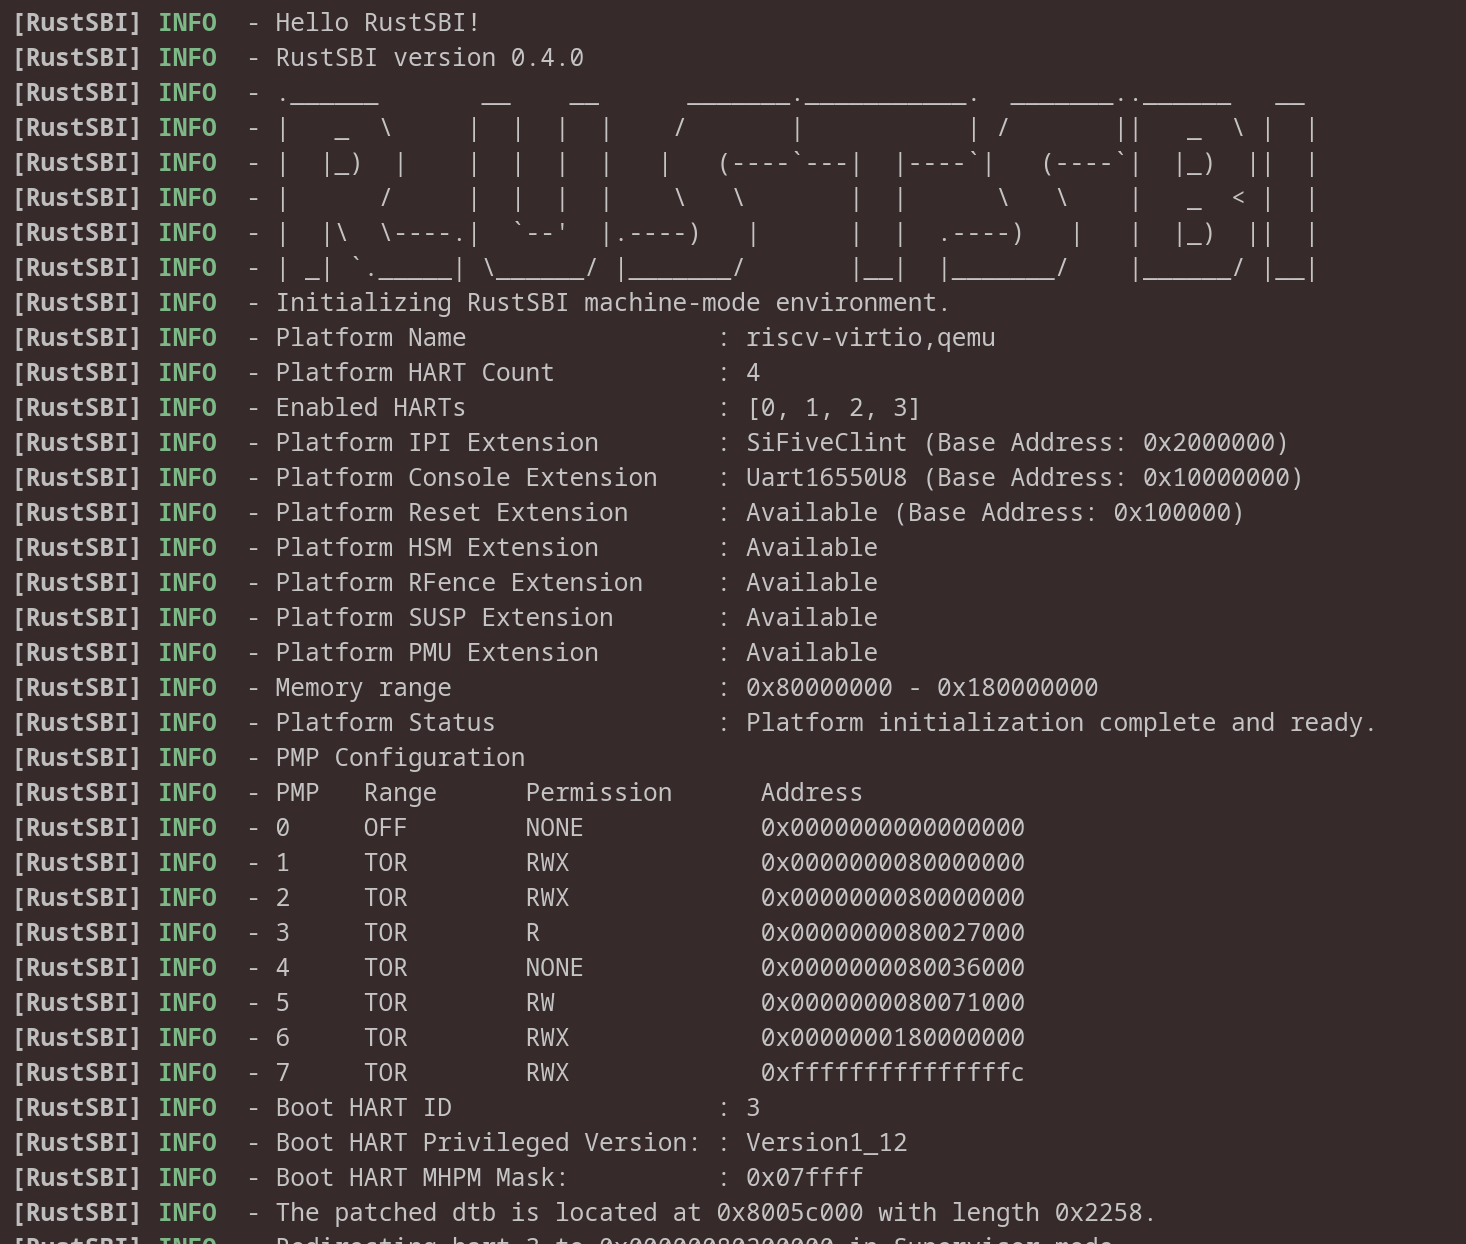
\includegraphics[width=1\linewidth]{hw_init.png}
		\caption{SBI固件初始化}
		\label{hw_init}
	\end{figure}
	
	当RustSBI完成底层硬件初始化后，系统控制权交还至EasyAda-SM以推进核心初始化逻辑。如图\ref{sm_init}所示，多hart的初始化日志交替输出，表明系统已成功唤醒并构建了SMP环境。鉴于RISC-V架构中各hart均拥有独立的控制与状态寄存器，EasyAda-SM确保了所有核心严格同步执行一致的安全策略配置，从而有效规避跨核越权访问等硬件级侧信道漏洞。
	
	\begin{figure}[!h]
		\centering		
		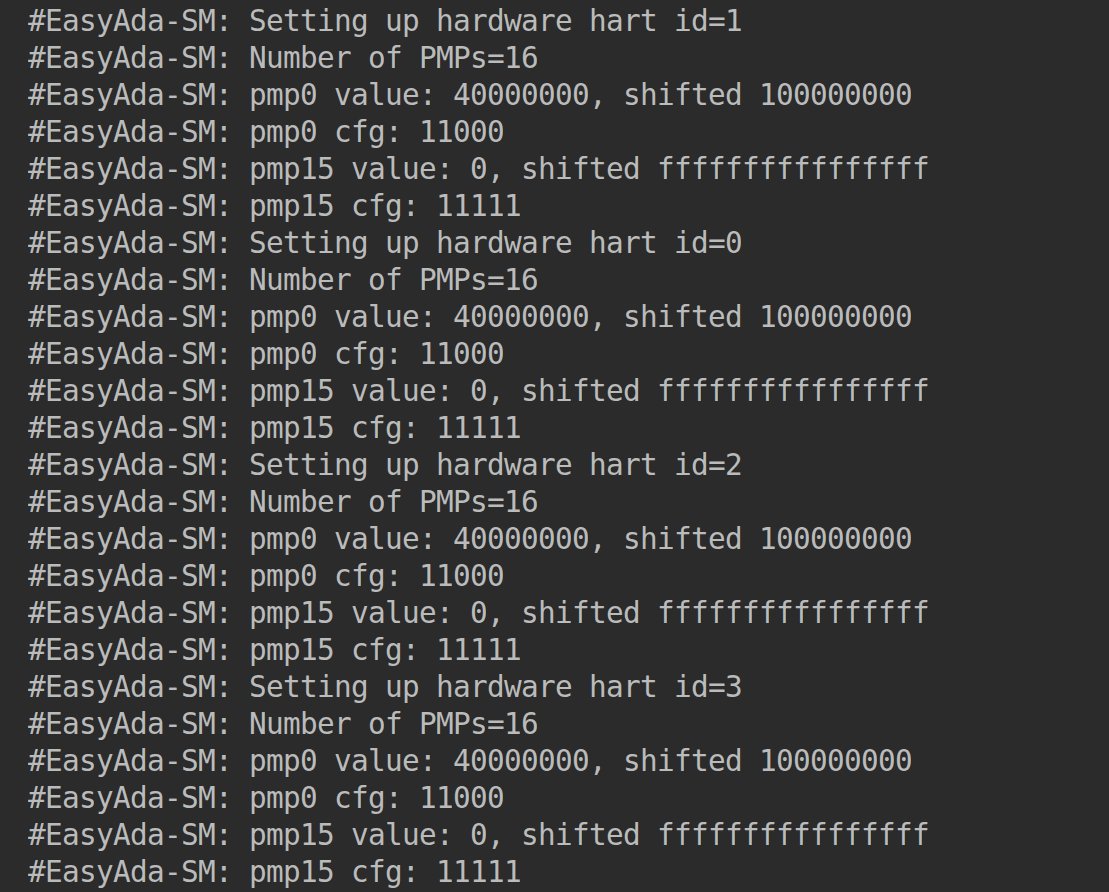
\includegraphics[width=1\linewidth]{sm_init.png}
		\caption{EasyAda-SM初始化测试}
		\label{sm_init}
	\end{figure}
	
	在全局内存隔离策略的构建上，测试环境中的Hart均支持16个PMP条目。EasyAda-SM利用最高优先级的条目划定SM的根安全区域，通过写入配置值0x18（即NAPOT匹配模式且权限为NONE），对预留的16MB安全监控器专有内存实施强制硬件隔离；同时，利用最低优先级的条目制定背景策略，授予系统默认访问公共物理内存与MMIO区域的权限。此外，为实现对RustSBI的最小化侵入式修改，系统保留了其独立的堆内存区；前述16MB预留空间的主体则被接管为EasyAda-SM的全局堆内存。上述初始化序列执行完毕后，控制权将正式移交至EasyAda-hypervisor，以开启虚拟化层的引导流程。
	
	\subsection{CVM安全启动测试}
	在普通VM提升为安全CVM时，需要完成CVM与EasyAda-SM的双向本地证明。本文模拟了以下三种边界情况进行安全启动流程测试：（1）CVM可信，平台可信；（2）CVM不可信，平台可信；（3）CVM可信，平台不可信。
	
	图\ref{cvm_tsm_trust}展示了可信CVM在可信平台上启动的基准情况。在该流程中，EasyAda-SM在接管VM提升请求后，对CVM的内存布局、内核镜像及FDT进行完整性度量。日志显示，系统计算得出的PCR4度量值与TAP中预置的参考值完全一致。本地证明成功后，SM向CVM安全注入TAP中存储的秘密，随后Linux内核成功引导。该结果验证了系统在理想状态下能够正确鉴权并启动合法CVM。
	\begin{figure}[!h]
		\centering		
		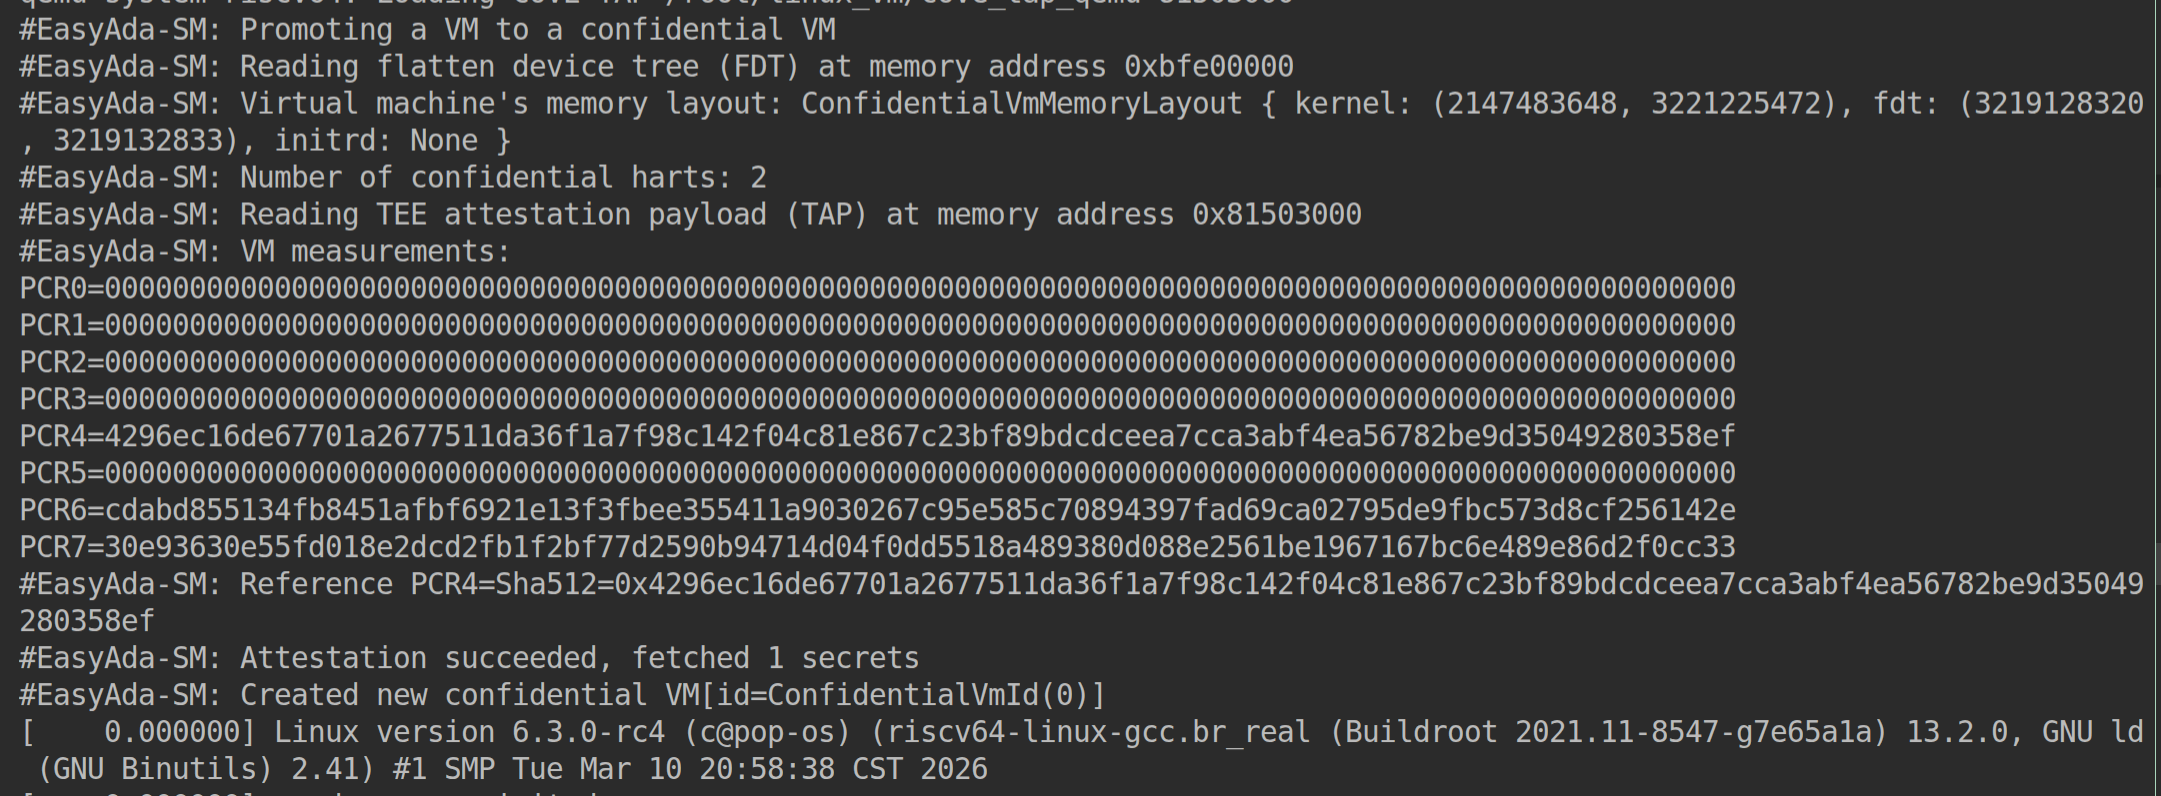
\includegraphics[width=1\linewidth]{cvm_tsm_trust.png}
		\caption{可信CVM在可信平台上启动测试}
		\label{cvm_tsm_trust}
	\end{figure}
	
	
	图\ref{untrust_cvm}展示了不可信CVM（例如内核镜像被恶意篡改）在可信平台上的启动被拦截过程。当EasyAda-SM对篡改后的CVM进行度量时，生成的PCR4值与预期参考值发生偏移。本地证明机制敏锐捕捉到该完整性破坏，抛出LocalAttestationFailed错误。随后，SM立即阻断引导流，拒绝为其分配执行权限，并将其从控制数据结构中安全移除。该测试证明了平台对恶意或受损CVM的有效识别与拦截能力。
	\begin{figure}[!h]
		\centering		
		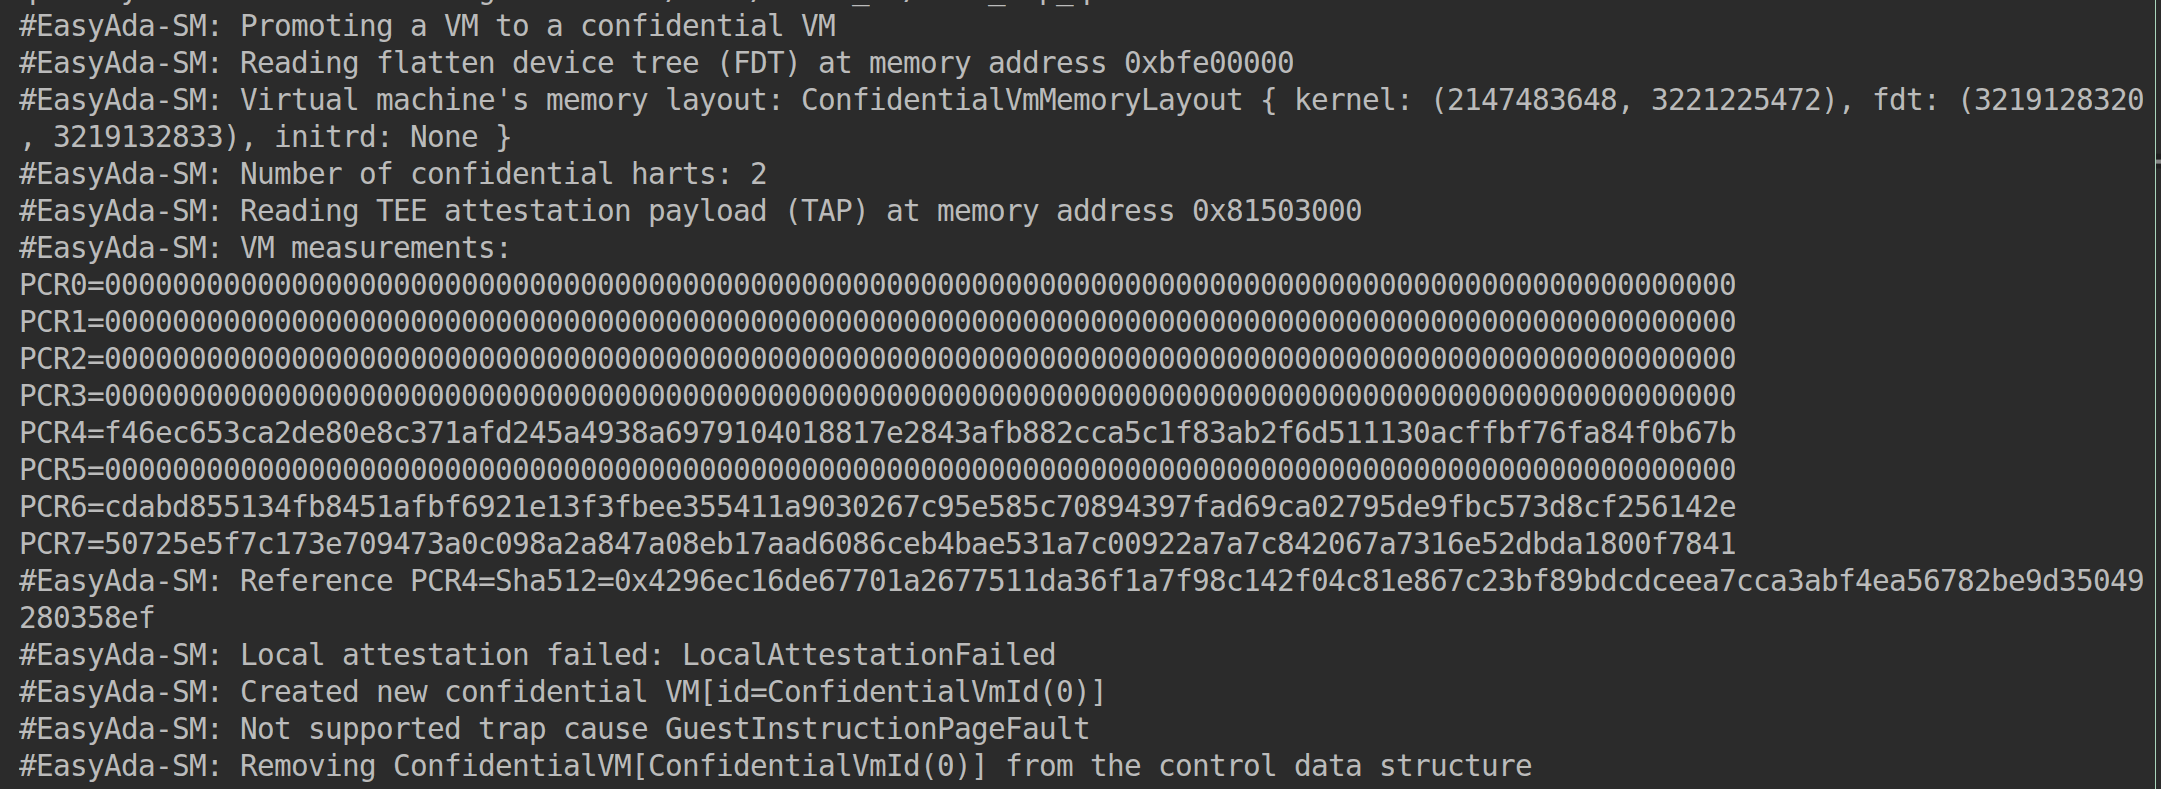
\includegraphics[width=1\linewidth]{untrust_cvm.png}
		\caption{不可信CVM在可信平台上启动测试}
		\label{untrust_cvm}
	\end{figure}
	
	图\ref{untrust_tsm}则验证了双向证明中的反向约束，即CVM可信但底层平台（EasyAda-SM或硬件运行环境）不可信的情况。在该场景下，当系统尝试读取并执行TAP以验证平台身份时，由于平台无法获取预期的用于解密的密钥，TAP解密失败并触发固件恐慌。SM随即中止启动流程并执行环境清理。此结果表明，EasyAda-trust架构有效防止了合法CVM在被攻陷或未授权的底层环境中运行，确保了机密计算环境的双向信任根基。	\begin{figure}[!h]
		\centering		
		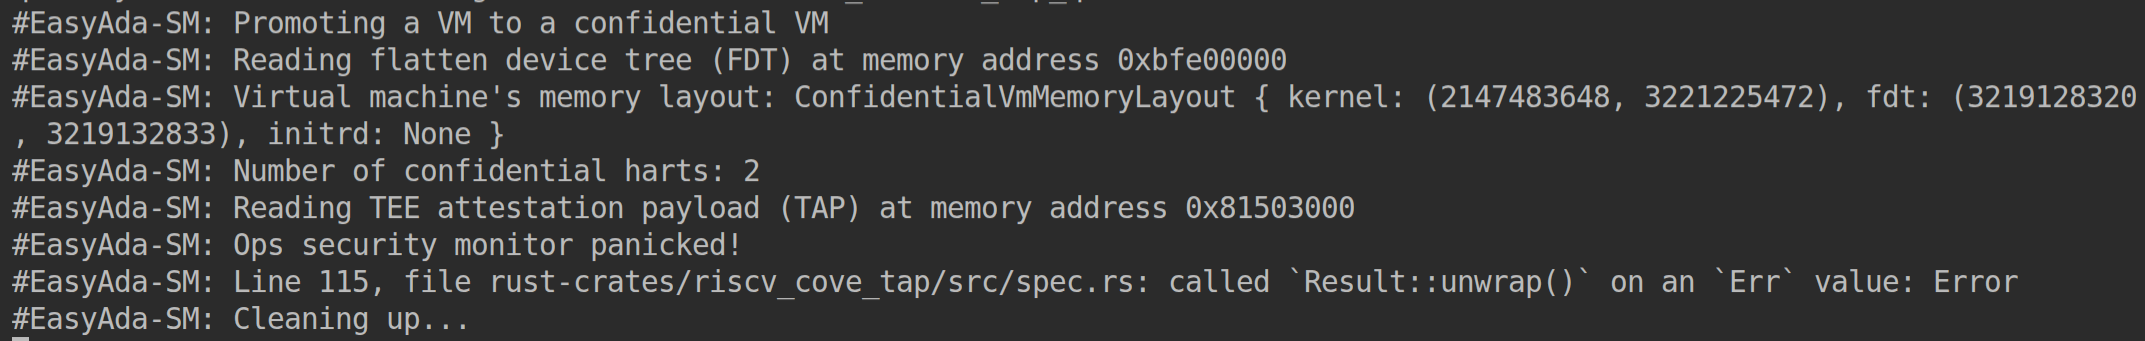
\includegraphics[width=1\linewidth]{untrust_tsm.png}
		\caption{可信CVM在不可信平台上启动测试}
		\label{untrust_tsm}
	\end{figure}
	
	\subsection{CVM性能测试}
	本节旨在全面评估EasyAda-trust架构在承载CVM时，TSM的引入对客户操作系统核心原语执行效率的影响。为了精准量化各项系统级操作的开销，本文选用LEBench\citess{lebench}作为核心测试套件。该套件能够精细评估进程调度、内存管理及基础I/O等系统调用的时延表现。
	

	鉴于仿真环境硬件时钟精度的客观限制，本测试对LEBench进行了批处理改造，将单次操作修改为批量循环执行后取平均值，以有效放大测量时延并确保数据的统计学精度。本文引入了以下三种对比基准：（1）原生 Linux，未启用虚拟化与TEE保护的裸金属物理执行环境，作为绝对性能上限的参照组；（2）普通虚拟机：运行于EasyAda-Hypervisor之上，受标准虚拟化调度但不具备EasyAda-SM内存隔离保护的虚拟机环境；（3）CVM，运行于EasyAda-trust架构之上，受EasyAda-SM全生命周期管理、内存强隔离及机密上下文切换保护的执行环境。
	
	如图\ref{lebench}所示，所有测试结果均以原生Linux环境的执行时延为基线进行归一化处理。数值越低代表操作时延越短、性能越优。具体分析如下：
	\begin{figure}[!h]
		\centering		
		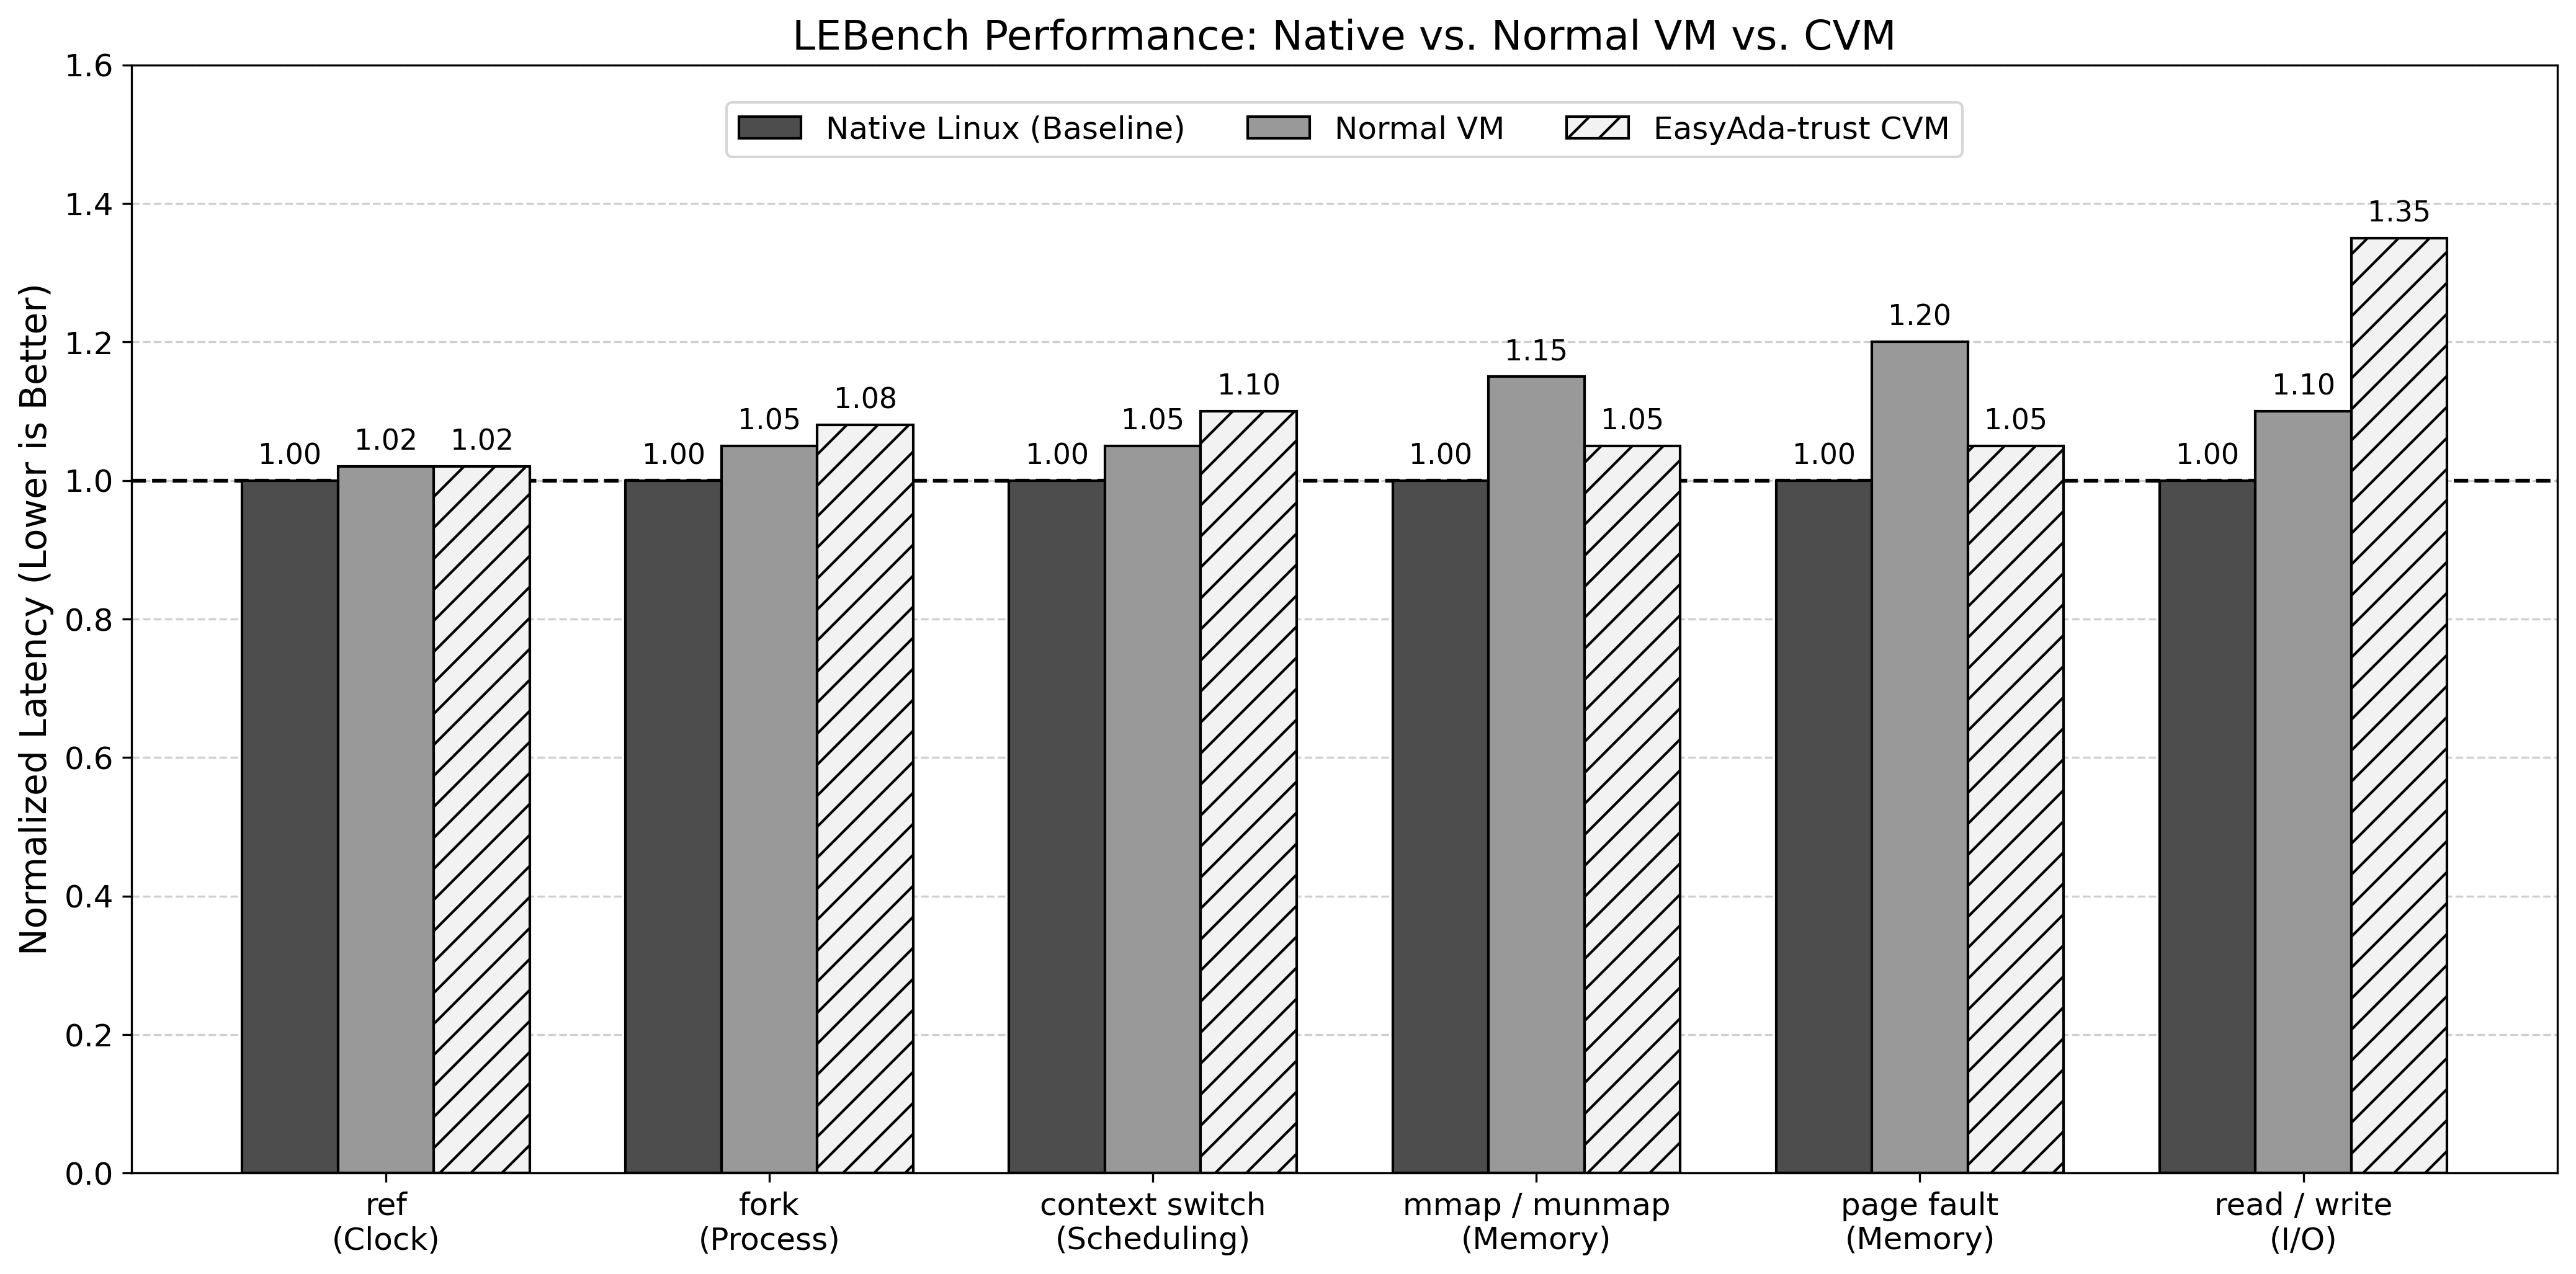
\includegraphics[width=1\linewidth]{lebench.png}
		\caption{LEBench测试结果}
		\label{lebench}
	\end{figure}
	
	在读取系统时钟的测试（ref）中，普通VM与CVM的归一化延迟几乎与物理裸机性能一致。这一表现归功于实验环境底层硬件对S态时钟中断扩展的完备支持，允许VM直接在VS态配置定时器并接收虚拟中断，规避了传统架构中需要陷入到M态进行注入的开销，这符合TSM直接将CVM时钟中断委派到VS态进行处理的设计。
	
	在内存分配与缺页异常处理上，普通虚拟机与CVM均表现出极高的效率，因为普通VM和CVM的运行期内存已在启动时一次性完成分配，由于二阶段页表在初始化时已建立完毕且不进行换出，虚拟机在运行期的缺页异常完全收敛于客户系统内部闭环处理，除了硬件固有的两阶段地址翻译开销外，并未在系统关键访存路径上引入任何额外的软件级运行时惩罚。
	
	在进程调度层面，CVM的时延略高于普通VM。LEBench测量的核心是虚拟机内部（VS与VU态之间）的用户态进程切换。虽然常规切换不会触发陷入TSM的行为，但在涉及跨执行环境的上下文协作时，需陷入TSM执行严苛的两阶段安全上下文切换、清理微架构残余状态，并动态重配安全内存视图，这导致了CVM侧可预期的性能衰减。
	
	\begin{figure}[!h]
		\centering		
		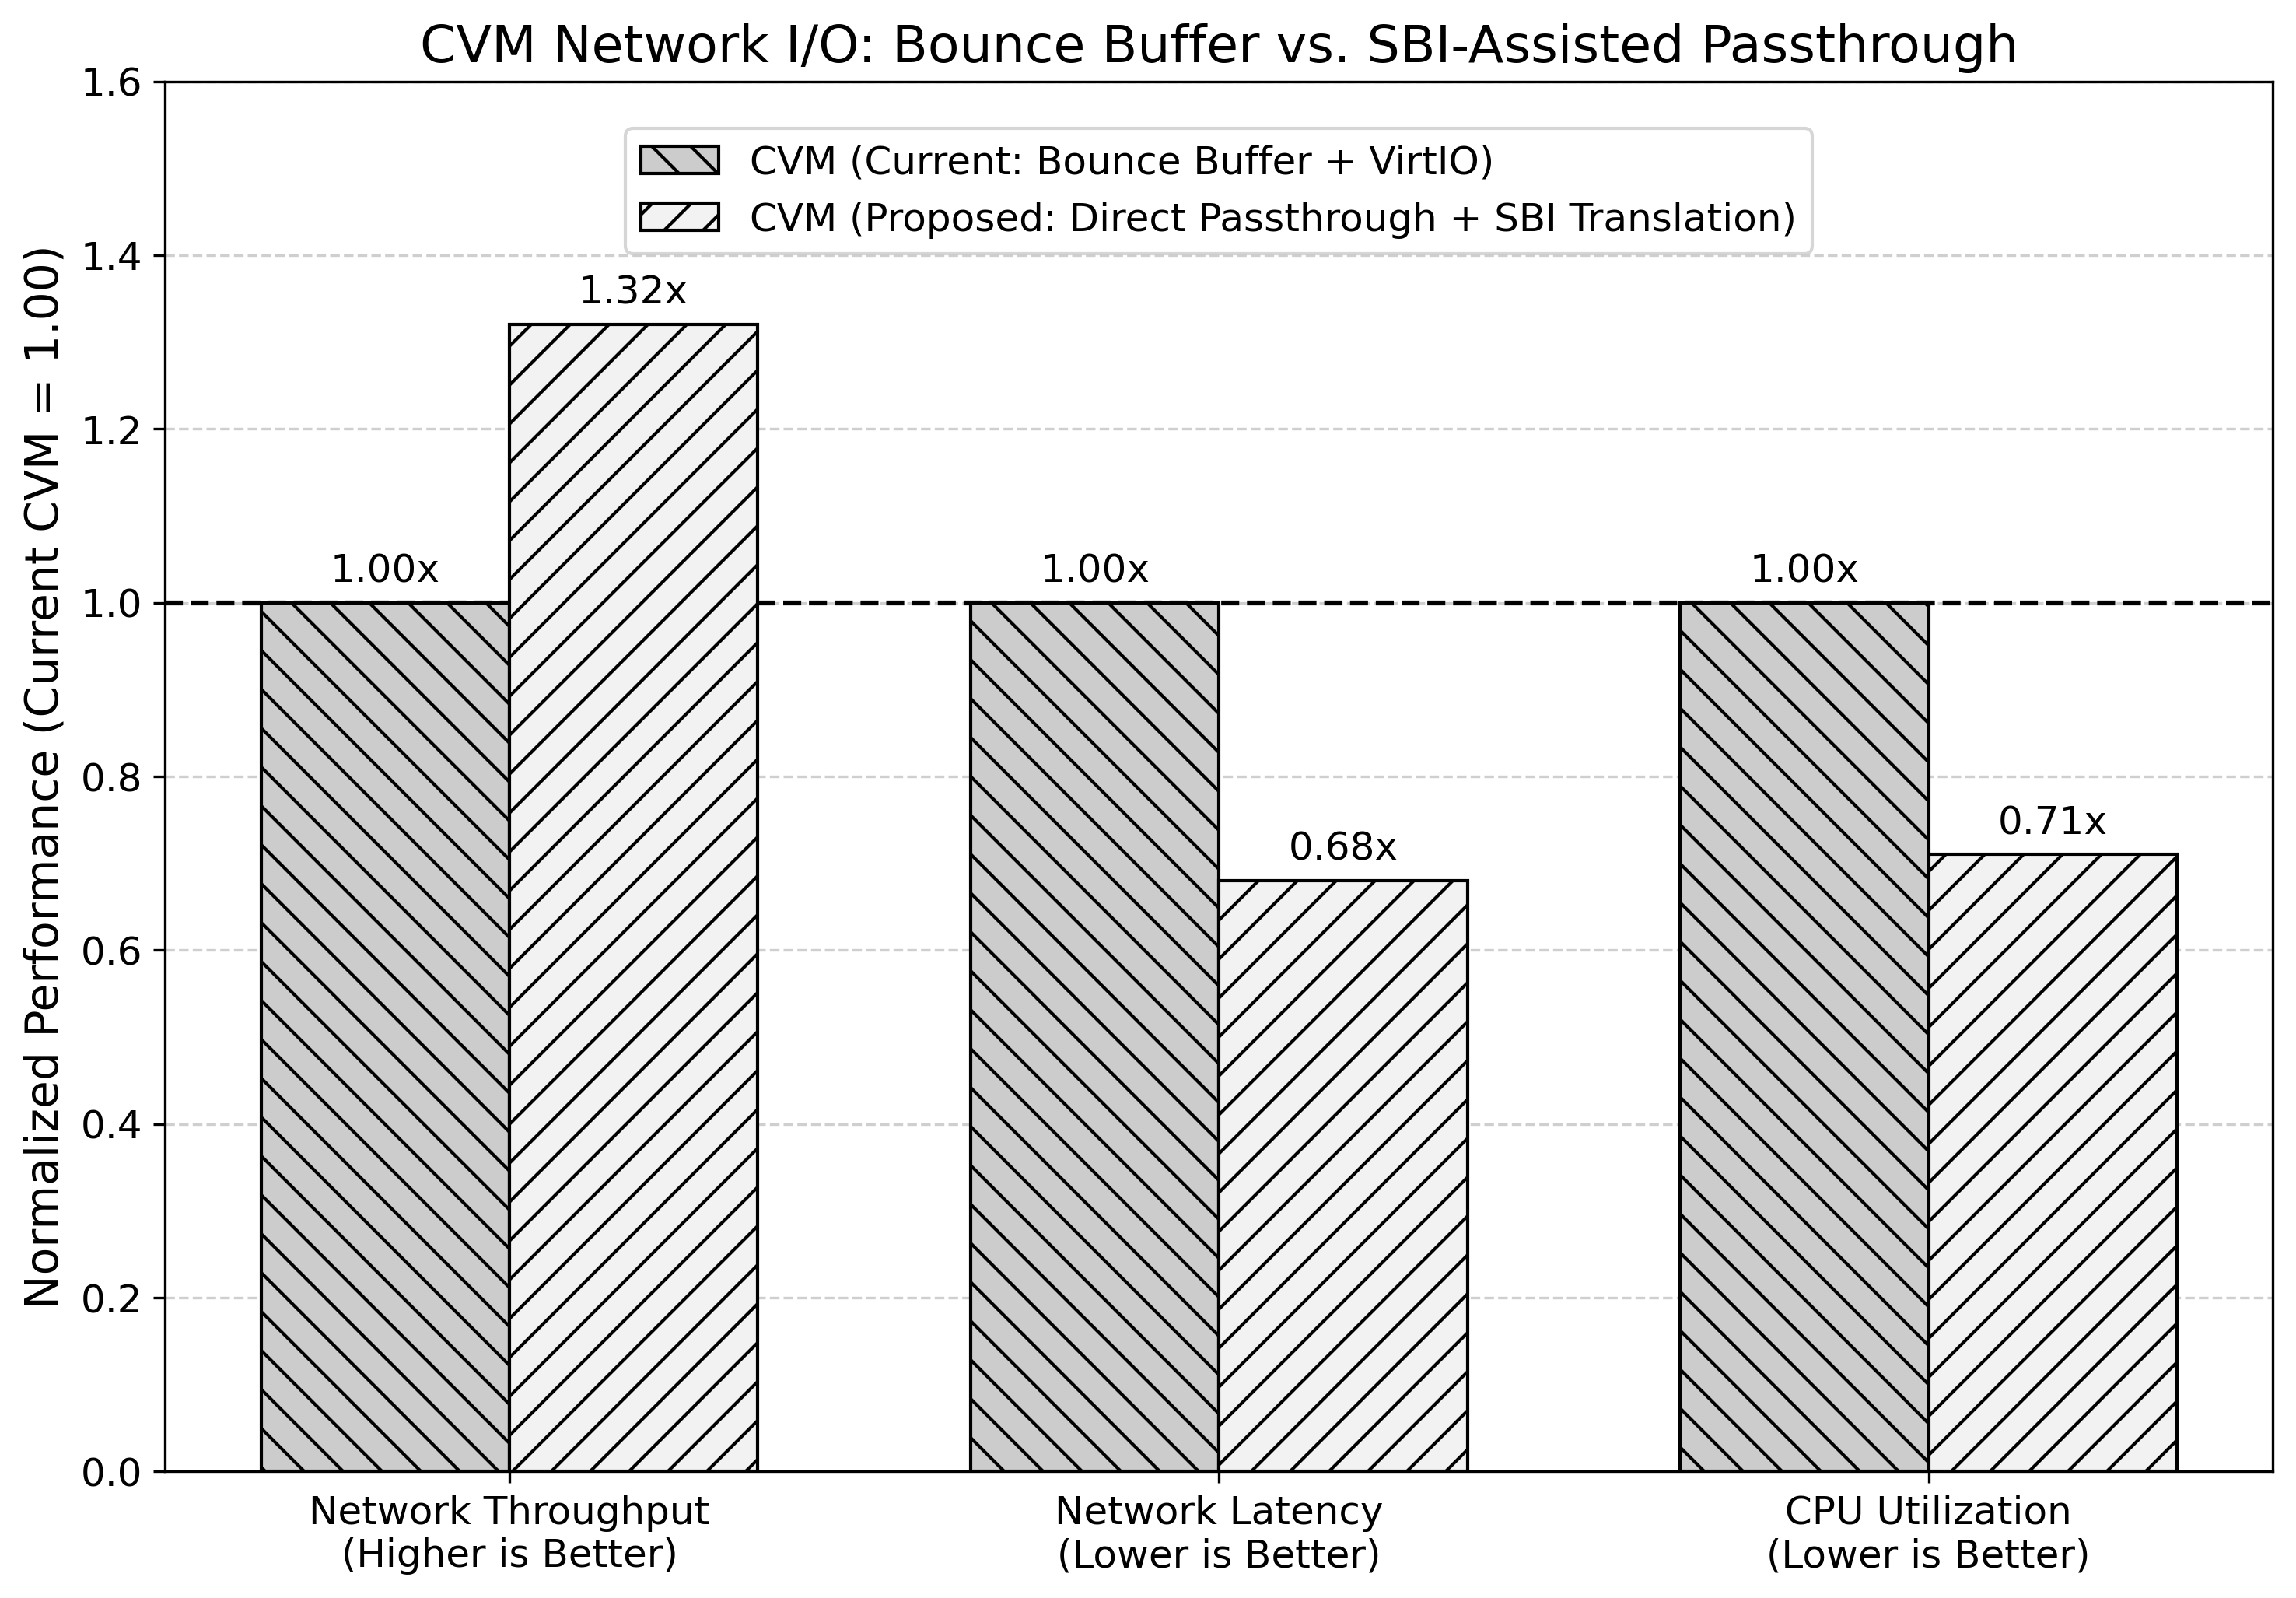
\includegraphics[width=0.7\linewidth]{io_passthrough.png}
		\caption{安全设备直通架构与半虚拟化机制（不可信共享内存）下的网卡I/O对比测试结果}
		\label{io_passthrough}
	\end{figure}
	
	基础I/O测试结果表明，底层设备路由架构对CVM性能具有决定性影响。在传统的全/半虚拟化架构下，为遵循严密的内存隔离模型，TSM阻断了不可信Hypervisor的DMA路径。这迫使CVM采用高开销的安全中转机制：I/O数据必须经历内部密码学加解密、向不可信共享缓冲区的多重拷贝，以及高频触发的TSM安全域上下文切换。此类数据冗余拷贝、微架构缓存失效与纯软件计算的叠加，共同导致该模式下I/O性能显著衰减。
	
	相比之下，图\ref{io_passthrough}展示了安全设备直通架构与半虚拟化机制（不可信共享内存）下的网卡I/O对比测试结果。该架构将受PMP保护的外设MMIO直接映射至CVM二阶段地址空间，并协同IOPMP扩展在总线级别实施抗DMA攻击的物理内存鉴权。机密应用得以合法旁路不可信软件中转栈，在免除高昂软件流加密开销的同时，实现了与受信异构硬件的零拷贝明文高速通信。
	
	\section{本章小结}
	本章对所提出的EasyAda-trust微内核可信虚拟化架构及其核心固件EasyAda-SM进行了系统性的定量评估与安全性验证。首先，通过Coremark与RV8基准测试证明了引入Rust内存安全机制后的EasyAda-SM具备极高的生态兼容性，且在核心计算场景下引入的额外运行时开销趋近于零。其次，验证了系统安全启动与双向本地证明机制的有效性，结果表明该机制能精准识别并拦截受损的虚拟机镜像与不可信的底层运行环境，确保了信任链的完整性。
	
	此外，通过LEBench微基准测试与网络I/O测试对CVM的全生命周期开销进行了深度剖析。数据表明，得益于静态安全内存预分配策略与Sstc硬件扩展的支持，CVM在系统时钟与内存管理等核心原语上实现了与原生实现相同的性能。而在面临物理隔离边界导致的I/O性能衰减时，本文提出的基于IOPMP扩展的安全设备直通架构，成功绕过了高昂的软件密码学计算与不可信内存中转栈，在保障系统隔离强度的同时，实现了异构外设的明文访问。综合而言，本系统在极致的内存安全保障与总体执行效能之间取得了较理想的架构折中。
	
	\chapter{总结和展望}
	\section{全文总结}
	虚拟化技术与可信执行环境作为优化资源利用、保障系统安全的核心技术手段，在物联网与端侧异构计算领域扮演着愈加重要的角色。机密虚拟机（CVM）作为现代TEE的演进方向，直接关系到用户敏感数据与AI模型资产的机密性、完整性及系统实时性。当前，基于x86和ARM架构的机密计算方案已广泛部署，但面向开源RISC-V架构的微内核机密虚拟化研究仍处于起步阶段，且传统C语言构建的底层固件面临严峻的内存安全威胁，因此该方向具有重大的学术与工程研究价值。
	
	本文围绕基于RISC-V架构的机密虚拟化方案实现与底层安全隔离机制展开系统性研究。基于RISC-V硬件虚拟化扩展（H扩展）、物理内存保护机制（PMP/IOPMP）以及自研微内核操作系统EasyAda及微内核虚拟化架构EasyAda-Hypervisor，设计并实现了基于微内核虚拟化架构的机密虚拟化架构EasyAda-trust及内存安全固件EasyAda-SM，并在QEMU仿真环境及多种基准测试套件下对其核心性质与性能开展了系统性评估。总体而言，本文主要贡献可概括为以下几点：
	
	1. 系统阐述了微内核虚拟化、TEE架构演进及其在异构计算环境下面临的安全挑战。在端侧与物联网系统中，硬件算力复用与AI数据隐私保护需求日益凸显。本文分析了CVM在实际系统中的关键作用，并指出引入Rust内存安全语言与RISC-V开放架构对于削减可信计算基（TCB）、消除内存漏洞及降低TEE准入门槛的重要意义。
	
	2. 针对底层安全监视器易受内存破坏漏洞威胁的痛点，本文提出并使用Rust语言从零构建了内存安全固件EasyAda-SM。该方案创新性地结合Rust的所有权机制设计了页分配器（Page Allocator），从编译期彻底杜绝了内存管理元数据被破坏的可能。同时，通过模块化分层设计，抽象出统一的物理内存保护原语与安全区域管理层，实现了不同类型Enclave与不可信组件间的物理级强隔离。
	
	3. 针对CVM全生命周期管理与异构安全扩展的需求，本文在微内核虚拟化方案EasyAda-Hypervisor的基础上设计实现了EasyAda-trust架构。通过将物理资源调度与安全内存映射鉴权进行深度解耦，实现了安全的CPU机密流上下文切换与二阶段页表隔离。在此基础上，本文结合IOPMP技术构建了防御恶意DMA攻击的总线屏障，并创新性地设计了加速器管理CVM，利用I/O半虚拟化技术实现了底层硬件加速器在不可信与机密环境间的安全时分复用。
	
	4. 本文在QEMU环境中对EasyAda-trust及其核心组件开展了多维度的定量评估与功能验证。测试结果表明，EasyAda-SM具备极高的生态兼容性，在核心计算负载（如Coremark与RV8 benchmark）下引入的性能损耗不到2\%；在安全机制验证方面，本文构建的基于本地证明的双向验证测试，成功验证了EasyAda-trust架构在CVM不可信或平台不可信等多种边界情况下的防御拦截能力。
	
	通过上述研究工作，本文提供了一种将微内核虚拟化技术与Rust内存安全固件深度融合的RISC-V机密计算解决方案。与已有的Keystone或Penglai等纯应用级/系统级TEE框架相比，本文聚焦于支持CVM抽象的虚拟机级强隔离，并在异构外设的机密复用维度提出了完整的软硬协同范式，为基于RISC-V架构的下一代端侧机密计算底座提供了一种高可靠、高可扩展的工程实现框架。

	\section{后续工作展望}
	尽管本文在RISC-V微内核机密虚拟化及安全隔离机制上取得了一定成果，但面向未来复杂系统的演进，仍有以下四个方向亟待深入研究与改进：

	1.多核机密并发调度与中断优化：当前跨环境上下文切换策略较为保守。未来将结合RISC-V高级中断架构，探索细粒度上下文感知与懒加载策略，优化核间中断与共享资源的并发控制，提升高并发负载下的吞吐量与实时响应能力。

	2. 真实硬件部署与直通开销优化：受限于硬件生态，本文评估主要基于QEMU。未来拟将系统移植至高阶RISC-V物理开发板进行全面压测。同时，针对IOPMP高频总线鉴权引入的DMA瓶颈，将探索基于硬件表项缓存或动态规则折叠的软硬协同算法，以降低物理访存损耗。

	3. 核心可信组件的形式化验证：尽管Rust从编译期消除了内存漏洞，但TSM的逻辑正确性仍需理论证明。未来将引入Isabelle/HOL等证明工具，对TSM的异常嵌套处理、二阶段页表映射等开展形式化验证，并扩展无干涉性证明，从理论层面夯实信任根。

	4. 异构计算生态与端到端总线安全：面向未来基于PCIe/CXL互连的片外独立加速器，现有机制难以防御总线窥探与重放攻击。未来将研究集成机密计算总线协议与内存加密引擎构建硬件级端到端加密链路，并拓展加速器CVM驱动生态，以原生支撑端侧大语言模型的机密推理。
	
	
	\acknowledgement
	%首先，我要向我的导师罗蕾教授致以最崇高的敬意和最诚挚的感谢。感谢您高屋建瓴的引领，将我带入嵌入式虚拟化与可信计算的广阔天地。同时，我要特别感谢肖堃老师。在无数个日夜里，是您给予了我最悉心的指导。从技术细节的反复推敲，到论文框架的字斟句酌，正是您的耐心答疑与无私帮助，使得本篇论文得以顺利成稿。
	
	%此外，我还要诚挚地感谢在求学期间给予我指导和帮助的所有老师与同学。感谢大家在日常科研中的探讨与启发，以及在系统开发和论文撰写过程中提供的宝贵建议与无私协助。正是因为有你们的陪伴与支持，这段充满挑战的求学道路才显得格外充实与温暖。
	
	%最后，我要将特别的感谢送给我的女朋友。在面对繁杂的代码、枯燥的实验以及论文反复修改的重压时，是你始终如一地陪伴在我身边。感谢你的理解与支持，你的鼓励和温柔抚平了我的焦虑，让这段漫长而艰辛的科研之旅不仅有代码的严谨，更充满了生活的色彩与期待。
	

	%% 参考文献部分
	% \nocite{*}% 为了便于在示例文档中展示参考文献而设，正式撰写时需要注释掉
	% \bibliographystyle{DissertUESTC}% 自v25.03.12版本后，参考文献风格文件由用户设定的论文类型选项自动确定，无需在此手动设置
	\bibliography{ref}

	% 附录起始位置
	\appendix
	
	\achievement % 仅研究生用

	%\begin{enumerate}[label={[\arabic*]}, leftmargin=2em, itemsep=0pt, parsep=0pt]
		
	%	\item Jinzhe L, Kun X, Lei L, et al. Easy adazone: A memory-safe physical memory isolation framework for risc-v[C]. 2025 22nd International Computer Conference on Wavelet Active Media Technology and Information Processing (ICCWAMTIP), 2025: 1-4.
		
	%\end{enumerate}

\end{document}